% Options for packages loaded elsewhere
\PassOptionsToPackage{unicode}{hyperref}
\PassOptionsToPackage{hyphens}{url}
%
\documentclass[
]{article}
\usepackage{lmodern}
\usepackage{amssymb,amsmath}
\usepackage{ifxetex,ifluatex}
\ifnum 0\ifxetex 1\fi\ifluatex 1\fi=0 % if pdftex
  \usepackage[T1]{fontenc}
  \usepackage[utf8]{inputenc}
  \usepackage{textcomp} % provide euro and other symbols
\else % if luatex or xetex
  \usepackage{unicode-math}
  \defaultfontfeatures{Scale=MatchLowercase}
  \defaultfontfeatures[\rmfamily]{Ligatures=TeX,Scale=1}
\fi
% Use upquote if available, for straight quotes in verbatim environments
\IfFileExists{upquote.sty}{\usepackage{upquote}}{}
\IfFileExists{microtype.sty}{% use microtype if available
  \usepackage[]{microtype}
  \UseMicrotypeSet[protrusion]{basicmath} % disable protrusion for tt fonts
}{}
\makeatletter
\@ifundefined{KOMAClassName}{% if non-KOMA class
  \IfFileExists{parskip.sty}{%
    \usepackage{parskip}
  }{% else
    \setlength{\parindent}{0pt}
    \setlength{\parskip}{6pt plus 2pt minus 1pt}}
}{% if KOMA class
  \KOMAoptions{parskip=half}}
\makeatother
\usepackage{xcolor}
\IfFileExists{xurl.sty}{\usepackage{xurl}}{} % add URL line breaks if available
\IfFileExists{bookmark.sty}{\usepackage{bookmark}}{\usepackage{hyperref}}
\hypersetup{
  pdftitle={Analysis 4: Mediation Analysis (Matched without Distance Adjustment)},
  pdfauthor={Fan Lu \& Gento Kato},
  hidelinks,
  pdfcreator={LaTeX via pandoc}}
\urlstyle{same} % disable monospaced font for URLs
\usepackage[margin=1in]{geometry}
\usepackage{color}
\usepackage{fancyvrb}
\newcommand{\VerbBar}{|}
\newcommand{\VERB}{\Verb[commandchars=\\\{\}]}
\DefineVerbatimEnvironment{Highlighting}{Verbatim}{commandchars=\\\{\}}
% Add ',fontsize=\small' for more characters per line
\usepackage{framed}
\definecolor{shadecolor}{RGB}{248,248,248}
\newenvironment{Shaded}{\begin{snugshade}}{\end{snugshade}}
\newcommand{\AlertTok}[1]{\textcolor[rgb]{0.94,0.16,0.16}{#1}}
\newcommand{\AnnotationTok}[1]{\textcolor[rgb]{0.56,0.35,0.01}{\textbf{\textit{#1}}}}
\newcommand{\AttributeTok}[1]{\textcolor[rgb]{0.77,0.63,0.00}{#1}}
\newcommand{\BaseNTok}[1]{\textcolor[rgb]{0.00,0.00,0.81}{#1}}
\newcommand{\BuiltInTok}[1]{#1}
\newcommand{\CharTok}[1]{\textcolor[rgb]{0.31,0.60,0.02}{#1}}
\newcommand{\CommentTok}[1]{\textcolor[rgb]{0.56,0.35,0.01}{\textit{#1}}}
\newcommand{\CommentVarTok}[1]{\textcolor[rgb]{0.56,0.35,0.01}{\textbf{\textit{#1}}}}
\newcommand{\ConstantTok}[1]{\textcolor[rgb]{0.00,0.00,0.00}{#1}}
\newcommand{\ControlFlowTok}[1]{\textcolor[rgb]{0.13,0.29,0.53}{\textbf{#1}}}
\newcommand{\DataTypeTok}[1]{\textcolor[rgb]{0.13,0.29,0.53}{#1}}
\newcommand{\DecValTok}[1]{\textcolor[rgb]{0.00,0.00,0.81}{#1}}
\newcommand{\DocumentationTok}[1]{\textcolor[rgb]{0.56,0.35,0.01}{\textbf{\textit{#1}}}}
\newcommand{\ErrorTok}[1]{\textcolor[rgb]{0.64,0.00,0.00}{\textbf{#1}}}
\newcommand{\ExtensionTok}[1]{#1}
\newcommand{\FloatTok}[1]{\textcolor[rgb]{0.00,0.00,0.81}{#1}}
\newcommand{\FunctionTok}[1]{\textcolor[rgb]{0.00,0.00,0.00}{#1}}
\newcommand{\ImportTok}[1]{#1}
\newcommand{\InformationTok}[1]{\textcolor[rgb]{0.56,0.35,0.01}{\textbf{\textit{#1}}}}
\newcommand{\KeywordTok}[1]{\textcolor[rgb]{0.13,0.29,0.53}{\textbf{#1}}}
\newcommand{\NormalTok}[1]{#1}
\newcommand{\OperatorTok}[1]{\textcolor[rgb]{0.81,0.36,0.00}{\textbf{#1}}}
\newcommand{\OtherTok}[1]{\textcolor[rgb]{0.56,0.35,0.01}{#1}}
\newcommand{\PreprocessorTok}[1]{\textcolor[rgb]{0.56,0.35,0.01}{\textit{#1}}}
\newcommand{\RegionMarkerTok}[1]{#1}
\newcommand{\SpecialCharTok}[1]{\textcolor[rgb]{0.00,0.00,0.00}{#1}}
\newcommand{\SpecialStringTok}[1]{\textcolor[rgb]{0.31,0.60,0.02}{#1}}
\newcommand{\StringTok}[1]{\textcolor[rgb]{0.31,0.60,0.02}{#1}}
\newcommand{\VariableTok}[1]{\textcolor[rgb]{0.00,0.00,0.00}{#1}}
\newcommand{\VerbatimStringTok}[1]{\textcolor[rgb]{0.31,0.60,0.02}{#1}}
\newcommand{\WarningTok}[1]{\textcolor[rgb]{0.56,0.35,0.01}{\textbf{\textit{#1}}}}
\usepackage{graphicx,grffile}
\makeatletter
\def\maxwidth{\ifdim\Gin@nat@width>\linewidth\linewidth\else\Gin@nat@width\fi}
\def\maxheight{\ifdim\Gin@nat@height>\textheight\textheight\else\Gin@nat@height\fi}
\makeatother
% Scale images if necessary, so that they will not overflow the page
% margins by default, and it is still possible to overwrite the defaults
% using explicit options in \includegraphics[width, height, ...]{}
\setkeys{Gin}{width=\maxwidth,height=\maxheight,keepaspectratio}
% Set default figure placement to htbp
\makeatletter
\def\fps@figure{htbp}
\makeatother
\setlength{\emergencystretch}{3em} % prevent overfull lines
\providecommand{\tightlist}{%
  \setlength{\itemsep}{0pt}\setlength{\parskip}{0pt}}
\setcounter{secnumdepth}{-\maxdimen} % remove section numbering
\usepackage{bookmark}
\usepackage{xltxtra}
\usepackage{zxjatype}
\usepackage[ipa]{zxjafont}

\title{Analysis 4: Mediation Analysis (Matched without Distance Adjustment)}
\author{Fan Lu \& Gento Kato}
\date{January 26, 2020}

\begin{document}
\maketitle

\hypertarget{preparation}{%
\section{Preparation}\label{preparation}}

\begin{Shaded}
\begin{Highlighting}[]
\CommentTok{## Clean Up Space}
\KeywordTok{rm}\NormalTok{(}\DataTypeTok{list=}\KeywordTok{ls}\NormalTok{())}

\CommentTok{## Set Working Directory (Automatically) ##}
\KeywordTok{require}\NormalTok{(rstudioapi); }\KeywordTok{require}\NormalTok{(rprojroot)}
\ControlFlowTok{if}\NormalTok{ (rstudioapi}\OperatorTok{::}\KeywordTok{isAvailable}\NormalTok{()}\OperatorTok{==}\OtherTok{TRUE}\NormalTok{) \{}
  \KeywordTok{setwd}\NormalTok{(}\KeywordTok{dirname}\NormalTok{(rstudioapi}\OperatorTok{::}\KeywordTok{getActiveDocumentContext}\NormalTok{()}\OperatorTok{$}\NormalTok{path)); }
\NormalTok{\} }
\NormalTok{projdir <-}\StringTok{ }\KeywordTok{find_root}\NormalTok{(}\KeywordTok{has_file}\NormalTok{(}\StringTok{"thisishome.txt"}\NormalTok{))}
\KeywordTok{cat}\NormalTok{(}\KeywordTok{paste}\NormalTok{(}\StringTok{"Working Directory Set to:}\CharTok{\textbackslash{}n}\StringTok{"}\NormalTok{,projdir))}
\end{Highlighting}
\end{Shaded}

\begin{verbatim}
## Working Directory Set to:
##  /home/gentok/GoogleDrive/Projects/Fan-Gento-Lab/ForeignerJapan
\end{verbatim}

\begin{Shaded}
\begin{Highlighting}[]
\KeywordTok{setwd}\NormalTok{(projdir)}

\CommentTok{## Matched/Unmatched Data Locations}
\NormalTok{datadir0 <-}\StringTok{ }\KeywordTok{paste0}\NormalTok{(projdir, }\StringTok{"/data/sifcct_unmatched_v5.rds"}\NormalTok{)}
\NormalTok{datadir1 <-}\StringTok{ }\KeywordTok{paste0}\NormalTok{(projdir, }\StringTok{"/data/sifcct_matched_1_all_v5.rds"}\NormalTok{)}
\NormalTok{datadir2 <-}\StringTok{ }\KeywordTok{paste0}\NormalTok{(projdir, }\StringTok{"/data/sifcct_matched_2_all_v5.rds"}\NormalTok{)}
\NormalTok{datadir3 <-}\StringTok{ }\KeywordTok{paste0}\NormalTok{(projdir, }\StringTok{"/data/sifcct_matched_3_all_v5.rds"}\NormalTok{)}
\NormalTok{datadir4 <-}\StringTok{ }\KeywordTok{paste0}\NormalTok{(projdir, }\StringTok{"/data/sifcct_matched_4_all_v5.rds"}\NormalTok{)}
\NormalTok{datadir5 <-}\StringTok{ }\KeywordTok{paste0}\NormalTok{(projdir, }\StringTok{"/data/sifcct_matched_5_all_v5.rds"}\NormalTok{)}
\end{Highlighting}
\end{Shaded}

\begin{Shaded}
\begin{Highlighting}[]
\CommentTok{## packages}
\KeywordTok{require}\NormalTok{(sandwich)}
\KeywordTok{require}\NormalTok{(lmtest)}
\KeywordTok{require}\NormalTok{(MASS)}
\KeywordTok{require}\NormalTok{(ggplot2)}
\KeywordTok{require}\NormalTok{(texreg)}
\KeywordTok{require}\NormalTok{(mediation)}

\CommentTok{##}
\NormalTok{vnmap <-}\StringTok{ }\KeywordTok{list}\NormalTok{(}\StringTok{"edu2"}\NormalTok{ =}\StringTok{ "University education"}\NormalTok{,}
              \StringTok{"female"}\NormalTok{ =}\StringTok{ "Gender (female)"}\NormalTok{,}
              \StringTok{"male"}\NormalTok{ =}\StringTok{ "Gender (male)"}\NormalTok{,}
              \StringTok{"age2"}\NormalTok{ =}\StringTok{ "Age 50s or older"}\NormalTok{,}
              \StringTok{"agex"}\NormalTok{ =}\StringTok{ "Age (by 10 years)"}\NormalTok{,}
              \StringTok{"knowledge"}\NormalTok{ =}\StringTok{ "Political Knowledge"}\NormalTok{,}
              \StringTok{"ideology"}\NormalTok{ =}\StringTok{ "Ideology"}\NormalTok{,}
              \StringTok{"ldpdpjft"}\NormalTok{ =}\StringTok{ "LDP -DPJ Feeling Thermometer"}\NormalTok{,}
              \StringTok{"familiarityFT_KOR"}\NormalTok{ =}\StringTok{ "South Korea Feeling Thermometer"}\NormalTok{,}
              \StringTok{"familiarityFT_CHN"}\NormalTok{ =}\StringTok{ "China Feeling Thermometer"}\NormalTok{,}
              \StringTok{"familiarityFT_USA"}\NormalTok{ =}\StringTok{ "United States Feeling Thermometer"}\NormalTok{,}
              \StringTok{"income"}\NormalTok{ =}\StringTok{ "Income"}\NormalTok{,}
              \StringTok{"edu2:female"}\NormalTok{ =}\StringTok{ "University * Female"}\NormalTok{,}
              \StringTok{"edu2:male"}\NormalTok{ =}\StringTok{ "University * Male"}\NormalTok{,}
              \StringTok{"edu2:age2"}\NormalTok{ =}\StringTok{ "University * >=50s"}\NormalTok{,}
              \StringTok{"edu2:agex"}\NormalTok{ =}\StringTok{ "University * Age"}\NormalTok{,}
              \StringTok{"edu2:female:age2"}\NormalTok{ =}\StringTok{ "University * Female * >=50s"}\NormalTok{,}
              \StringTok{"edu2:male:age2"}\NormalTok{ =}\StringTok{ "University * Male * >=50s"}\NormalTok{,}
              \StringTok{"edu2:female:agex"}\NormalTok{ =}\StringTok{ "University * Female * Age"}\NormalTok{,}
              \StringTok{"edu2:male:agex"}\NormalTok{ =}\StringTok{ "University * Male * Age"}\NormalTok{,}
              \StringTok{"female:knowledge"}\NormalTok{ =}\StringTok{ "Knowledge * Female"}\NormalTok{,}
              \StringTok{"male:knowledge"}\NormalTok{ =}\StringTok{ "Knowledge * Male"}\NormalTok{,}
              \StringTok{"age2:knowledge"}\NormalTok{ =}\StringTok{ "Knowledge * >=50s"}\NormalTok{,}
              \StringTok{"agex:knowledge"}\NormalTok{ =}\StringTok{ "Knowledge * Age"}\NormalTok{,}
              \StringTok{"female:age2:knowledge"}\NormalTok{ =}\StringTok{ "Knowledge * Female * >=50s"}\NormalTok{,}
              \StringTok{"male:age2:knowledge"}\NormalTok{ =}\StringTok{ "Knowledge * Male * >=50s"}\NormalTok{,}
              \StringTok{"female:agex:knowledge"}\NormalTok{ =}\StringTok{ "Knowledge * Female * Age"}\NormalTok{,}
              \StringTok{"male:agex:knowledge"}\NormalTok{ =}\StringTok{ "Knowledge * Male * Age"}\NormalTok{,}
              \StringTok{"female:ideology"}\NormalTok{ =}\StringTok{ "Ideology * Female"}\NormalTok{,}
              \StringTok{"male:ideology"}\NormalTok{ =}\StringTok{ "Ideology * Male"}\NormalTok{,}
              \StringTok{"age2:ideology"}\NormalTok{ =}\StringTok{ "Ideology * >=50s"}\NormalTok{,}
              \StringTok{"agex:ideology"}\NormalTok{ =}\StringTok{ "Ideology * Age"}\NormalTok{,}
              \StringTok{"female:age2:ideology"}\NormalTok{ =}\StringTok{ "Ideology * Female * >=50s"}\NormalTok{,}
              \StringTok{"male:age2:ideology"}\NormalTok{ =}\StringTok{ "Ideology * Male * >=50s"}\NormalTok{,}
              \StringTok{"female:agex:ideology"}\NormalTok{ =}\StringTok{ "Ideology * Female * Age"}\NormalTok{,}
              \StringTok{"male:agex:ideology"}\NormalTok{ =}\StringTok{ "Ideology * Male * Age"}\NormalTok{,}
              \StringTok{"female:ldpdpjft"}\NormalTok{ =}\StringTok{ "LDP - DPJ FT * Female"}\NormalTok{,}
              \StringTok{"male:ldpdpjft"}\NormalTok{ =}\StringTok{ "LDP - DPJ FT * Male"}\NormalTok{,}
              \StringTok{"age2:ldpdpjft"}\NormalTok{ =}\StringTok{ "LDP - DPJ FT * >=50s"}\NormalTok{,}
              \StringTok{"agex:ldpdpjft"}\NormalTok{ =}\StringTok{ "LDP - DPJ FT * Age"}\NormalTok{,}
              \StringTok{"female:age2:ldpdpjft"}\NormalTok{ =}\StringTok{ "LDP - DPJ FT * Female * >=50s"}\NormalTok{,}
              \StringTok{"male:age2:ldpdpjft"}\NormalTok{ =}\StringTok{ "LDP - DPJ FT * Male * >=50s"}\NormalTok{,}
              \StringTok{"female:agex:ldpdpjft"}\NormalTok{ =}\StringTok{ "LDP - DPJ FT * Female * Age"}\NormalTok{,}
              \StringTok{"male:agex:ldpdpjft"}\NormalTok{ =}\StringTok{ "LDP - DPJ FT * Male * Age"}\NormalTok{,}
              \StringTok{"female:familiarityFT_KOR"}\NormalTok{ =}\StringTok{ "South Korea FT * Female"}\NormalTok{,}
              \StringTok{"male:familiarityFT_KOR"}\NormalTok{ =}\StringTok{ "South Korea FT * Male"}\NormalTok{,}
              \StringTok{"age2:familiarityFT_KOR"}\NormalTok{ =}\StringTok{ "South Korea FT * >=50s"}\NormalTok{,}
              \StringTok{"agex:familiarityFT_KOR"}\NormalTok{ =}\StringTok{ "South Korea FT * Age"}\NormalTok{,}
              \StringTok{"female:age2:familiarityFT_KOR"}\NormalTok{ =}\StringTok{ "South Korea FT * Female * >=50s"}\NormalTok{,}
              \StringTok{"male:age2:familiarityFT_KOR"}\NormalTok{ =}\StringTok{ "South Korea FT * Male * >=50s"}\NormalTok{,}
              \StringTok{"female:agex:familiarityFT_KOR"}\NormalTok{ =}\StringTok{ "South Korea FT * Female * Age"}\NormalTok{,}
              \StringTok{"male:agex:familiarityFT_KOR"}\NormalTok{ =}\StringTok{ "South Korea FT * Male * Age"}\NormalTok{,}
              \StringTok{"female:familiarityFT_CHN"}\NormalTok{ =}\StringTok{ "China FT * Female"}\NormalTok{,}
              \StringTok{"male:familiarityFT_CHN"}\NormalTok{ =}\StringTok{ "China FT * Male"}\NormalTok{,}
              \StringTok{"age2:familiarityFT_CHN"}\NormalTok{ =}\StringTok{ "China FT * >=50s"}\NormalTok{,}
              \StringTok{"agex:familiarityFT_CHN"}\NormalTok{ =}\StringTok{ "China FT * Age"}\NormalTok{,}
              \StringTok{"female:age2:familiarityFT_CHN"}\NormalTok{ =}\StringTok{ "China FT * Female * >=50s"}\NormalTok{,}
              \StringTok{"male:age2:familiarityFT_CHN"}\NormalTok{ =}\StringTok{ "China FT * Male * >=50s"}\NormalTok{,}
              \StringTok{"female:agex:familiarityFT_CHN"}\NormalTok{ =}\StringTok{ "China FT * Female * Age"}\NormalTok{,}
              \StringTok{"male:agex:familiarityFT_CHN"}\NormalTok{ =}\StringTok{ "China FT * Male * Age"}\NormalTok{,}
              \StringTok{"female:familiarityFT_USA"}\NormalTok{ =}\StringTok{ "United States FT * Female"}\NormalTok{,}
              \StringTok{"male:familiarityFT_USA"}\NormalTok{ =}\StringTok{ "United States FT * Male"}\NormalTok{,}
              \StringTok{"age2:familiarityFT_USA"}\NormalTok{ =}\StringTok{ "United States FT * >=50s"}\NormalTok{,}
              \StringTok{"agex:familiarityFT_USA"}\NormalTok{ =}\StringTok{ "United States FT * Age"}\NormalTok{,}
              \StringTok{"female:age2:familiarityFT_USA"}\NormalTok{ =}\StringTok{ "United States FT * Female * >=50s"}\NormalTok{,}
              \StringTok{"male:age2:familiarityFT_USA"}\NormalTok{ =}\StringTok{ "United States FT * Male * >=50s"}\NormalTok{,}
              \StringTok{"female:agex:familiarityFT_USA"}\NormalTok{ =}\StringTok{ "United States FT * Female * Age"}\NormalTok{,}
              \StringTok{"male:agex:familiarityFT_USA"}\NormalTok{ =}\StringTok{ "United States FT * Male * Age"}\NormalTok{,}
              \StringTok{"female:income"}\NormalTok{ =}\StringTok{ "Income * Female"}\NormalTok{,}
              \StringTok{"male:income"}\NormalTok{ =}\StringTok{ "Income * Male"}\NormalTok{,}
              \StringTok{"age2:income"}\NormalTok{ =}\StringTok{ "Income * >=50s"}\NormalTok{,}
              \StringTok{"age:income"}\NormalTok{ =}\StringTok{ "Income * Age"}\NormalTok{,}
              \StringTok{"female:age2:income"}\NormalTok{ =}\StringTok{ "Income * Female * >=50s"}\NormalTok{,}
              \StringTok{"male:age2:income"}\NormalTok{ =}\StringTok{ "Income * Male * >=50s"}\NormalTok{,}
              \StringTok{"female:agex:income"}\NormalTok{ =}\StringTok{ "Income * Female * Age"}\NormalTok{,}
              \StringTok{"male:agex:income"}\NormalTok{ =}\StringTok{ "Income * Male * Age"}\NormalTok{,}
              \StringTok{"female:age2"}\NormalTok{ =}\StringTok{ "Female * >=50s"}\NormalTok{,}
              \StringTok{"male:age2"}\NormalTok{ =}\StringTok{ "Male * >=50s"}\NormalTok{,}
              \StringTok{"female:agex"}\NormalTok{ =}\StringTok{ "Female * Age"}\NormalTok{,}
              \StringTok{"male:agex"}\NormalTok{ =}\StringTok{ "Male * Age"}\NormalTok{,}
              \StringTok{"agecatMiddle Aged (40-50s)"}\NormalTok{ =}\StringTok{ "Middle Aged (40-50s)"}\NormalTok{,}
              \StringTok{"agecatElder (>=60s)"}\NormalTok{ =}\StringTok{ "Elder (>=60s)"}\NormalTok{,}
              \StringTok{"lvpr"}\NormalTok{ =}\StringTok{ "% of Life Residing Locally (zip)"}\NormalTok{,}
              \StringTok{"zip_did"}\NormalTok{ =}\StringTok{ "DID residence (zip)"}\NormalTok{,}
              \StringTok{"sqrt(c10_sreg_fper)"}\NormalTok{ =}\StringTok{ "Foreigner % sqrt. (zip)"}\NormalTok{,}
              \StringTok{"c10_sreg_edu_ugsP"}\NormalTok{ =}\StringTok{ "University % (zip)"}\NormalTok{,}
              \StringTok{"I(c10_sreg_edu_ugsP/10)"}\NormalTok{ =}\StringTok{ "University % by 10% (zip)"}\NormalTok{,}
              \StringTok{"didper"}\NormalTok{ =}\StringTok{ "DID proportion (mun.)"}\NormalTok{,}
              \StringTok{"sqrt(c10_mun_fper)"}\NormalTok{ =}\StringTok{ "Foreigner % sqrt. (mun.)"}\NormalTok{,}
              \StringTok{"I(c10_mun_edu_ugsP/10)"}\NormalTok{ =}\StringTok{ "University % by 10% (mun.)"}\NormalTok{,}
              \StringTok{"c10_mun_edu_ugsP"}\NormalTok{ =}\StringTok{ "University % (mun.)"}\NormalTok{)}
\end{Highlighting}
\end{Shaded}

\hypertarget{models}{%
\section{Models}\label{models}}

\hypertarget{sifcct-matched-without-distance-adjustment}{%
\subsection{SIFCCT (Matched without Distance
Adjustment)}\label{sifcct-matched-without-distance-adjustment}}

\begin{Shaded}
\begin{Highlighting}[]
\NormalTok{sifcct <-}\StringTok{ }\KeywordTok{readRDS}\NormalTok{(datadir1)}
\NormalTok{sifcct}\OperatorTok{$}\NormalTok{agex <-}\StringTok{ }\NormalTok{sifcct}\OperatorTok{$}\NormalTok{age}\OperatorTok{/}\DecValTok{10} \OperatorTok{-}\StringTok{ }\FloatTok{4.5}
\NormalTok{sifcct}\OperatorTok{$}\NormalTok{ldpdpjft <-}\StringTok{ }\NormalTok{original}\OperatorTok{$}\NormalTok{ldpdpjft[}\KeywordTok{match}\NormalTok{(}\KeywordTok{paste}\NormalTok{(sifcct}\OperatorTok{$}\NormalTok{id,sifcct}\OperatorTok{$}\NormalTok{wave),}\KeywordTok{paste}\NormalTok{(original}\OperatorTok{$}\NormalTok{id,original}\OperatorTok{$}\NormalTok{wave))]}
\KeywordTok{summary}\NormalTok{(sifcct}\OperatorTok{$}\NormalTok{ldpdpjft)}
\NormalTok{sifcct}\OperatorTok{$}\NormalTok{income <-}\StringTok{ }\NormalTok{original}\OperatorTok{$}\NormalTok{income[}\KeywordTok{match}\NormalTok{(}\KeywordTok{paste}\NormalTok{(sifcct}\OperatorTok{$}\NormalTok{id,sifcct}\OperatorTok{$}\NormalTok{wave),}\KeywordTok{paste}\NormalTok{(original}\OperatorTok{$}\NormalTok{id,original}\OperatorTok{$}\NormalTok{wave))]}
\KeywordTok{summary}\NormalTok{(sifcct}\OperatorTok{$}\NormalTok{income)}
\end{Highlighting}
\end{Shaded}

\hypertarget{knowledge}{%
\subsubsection{Knowledge}\label{knowledge}}

\begin{Shaded}
\begin{Highlighting}[]
\CommentTok{## Outcome Model }
\NormalTok{s1mout01_1C <-}\StringTok{ }\KeywordTok{lm}\NormalTok{(foreignsuff  }\OperatorTok{~}\StringTok{ }\NormalTok{edu2}\OperatorTok{*}\NormalTok{male}\OperatorTok{*}\NormalTok{agex }\OperatorTok{+}\StringTok{ }\NormalTok{knowledge}\OperatorTok{*}\NormalTok{male}\OperatorTok{*}\NormalTok{agex }\OperatorTok{+}\StringTok{ }\NormalTok{lvpr }\OperatorTok{+}\StringTok{  }
\StringTok{                    }\NormalTok{zip_did }\OperatorTok{+}\StringTok{ }\KeywordTok{sqrt}\NormalTok{(c10_sreg_fper) }\OperatorTok{+}\StringTok{ }\KeywordTok{I}\NormalTok{(c10_sreg_edu_ugsP}\OperatorTok{/}\DecValTok{10}\NormalTok{) }\OperatorTok{+}\StringTok{ }
\StringTok{                    }\NormalTok{didper }\OperatorTok{+}\StringTok{ }\KeywordTok{sqrt}\NormalTok{(c10_mun_fper) }\OperatorTok{+}\StringTok{ }\KeywordTok{I}\NormalTok{(c10_mun_edu_ugsP}\OperatorTok{/}\DecValTok{10}\NormalTok{) }\OperatorTok{+}\StringTok{ }
\StringTok{                    }\KeywordTok{as.factor}\NormalTok{(wave), }\DataTypeTok{data=}\NormalTok{sifcct)}

\CommentTok{## Mediator Model}
\NormalTok{s1mm01_1C <-}\StringTok{ }\KeywordTok{lm}\NormalTok{(knowledge  }\OperatorTok{~}\StringTok{ }\NormalTok{edu2}\OperatorTok{*}\NormalTok{male}\OperatorTok{*}\NormalTok{agex }\OperatorTok{+}\StringTok{ }\NormalTok{lvpr }\OperatorTok{+}\StringTok{  }
\StringTok{                    }\NormalTok{zip_did }\OperatorTok{+}\StringTok{ }\KeywordTok{sqrt}\NormalTok{(c10_sreg_fper) }\OperatorTok{+}\StringTok{ }\KeywordTok{I}\NormalTok{(c10_sreg_edu_ugsP}\OperatorTok{/}\DecValTok{10}\NormalTok{) }\OperatorTok{+}\StringTok{ }
\StringTok{                  }\NormalTok{didper }\OperatorTok{+}\StringTok{ }\KeywordTok{sqrt}\NormalTok{(c10_mun_fper) }\OperatorTok{+}\StringTok{ }\KeywordTok{I}\NormalTok{(c10_mun_edu_ugsP}\OperatorTok{/}\DecValTok{10}\NormalTok{) }\OperatorTok{+}\StringTok{ }
\StringTok{                  }\KeywordTok{as.factor}\NormalTok{(wave), }\DataTypeTok{data=}\NormalTok{sifcct)}

\CommentTok{## Table}
\KeywordTok{screenreg}\NormalTok{(}\KeywordTok{list}\NormalTok{(s1mm01_1C,s1mout01_1C), }\DataTypeTok{digits =} \DecValTok{4}\NormalTok{, }\DataTypeTok{single.row =}\NormalTok{ T,}
          \DataTypeTok{override.se =} \KeywordTok{list}\NormalTok{(}\KeywordTok{coeftest}\NormalTok{(s1mm01_1C,}\DataTypeTok{vcov.=}\KeywordTok{vcovHC}\NormalTok{(s1mm01_1C))[,}\DecValTok{2}\NormalTok{],}
                             \KeywordTok{coeftest}\NormalTok{(s1mout01_1C,}\DataTypeTok{vcov.=}\KeywordTok{vcovHC}\NormalTok{(s1mout01_1C))[,}\DecValTok{2}\NormalTok{]),}
          \DataTypeTok{override.pvalues =} \KeywordTok{list}\NormalTok{(}\KeywordTok{coeftest}\NormalTok{(s1mm01_1C,}\DataTypeTok{vcov.=}\KeywordTok{vcovHC}\NormalTok{(s1mm01_1C))[,}\DecValTok{4}\NormalTok{],}
                                  \KeywordTok{coeftest}\NormalTok{(s1mout01_1C,}\DataTypeTok{vcov.=}\KeywordTok{vcovHC}\NormalTok{(s1mout01_1C))[,}\DecValTok{4}\NormalTok{]),}
          \DataTypeTok{omit.coef =} \StringTok{"(wave)"}\NormalTok{, }\DataTypeTok{stars =} \KeywordTok{c}\NormalTok{(}\FloatTok{0.1}\NormalTok{,}\FloatTok{0.05}\NormalTok{,}\FloatTok{0.01}\NormalTok{,}\FloatTok{0.001}\NormalTok{), }\DataTypeTok{symbol =} \StringTok{"+"}\NormalTok{,}
          \DataTypeTok{custom.coef.map =}\NormalTok{ vnmap, }
          \DataTypeTok{custom.model.names =} \KeywordTok{c}\NormalTok{(}\StringTok{"Mediator"}\NormalTok{,}\StringTok{"Outcome"}\NormalTok{))}
\end{Highlighting}
\end{Shaded}

\hypertarget{ideology}{%
\subsubsection{Ideology}\label{ideology}}

\begin{Shaded}
\begin{Highlighting}[]
\CommentTok{## Outcome Model }
\NormalTok{s1mout02_1C <-}\StringTok{ }\KeywordTok{lm}\NormalTok{(foreignsuff  }\OperatorTok{~}\StringTok{ }\NormalTok{edu2}\OperatorTok{*}\NormalTok{male}\OperatorTok{*}\NormalTok{agex }\OperatorTok{+}\StringTok{ }\NormalTok{ideology}\OperatorTok{*}\NormalTok{male}\OperatorTok{*}\NormalTok{agex }\OperatorTok{+}\StringTok{ }\NormalTok{lvpr }\OperatorTok{+}\StringTok{  }
\StringTok{                    }\NormalTok{zip_did }\OperatorTok{+}\StringTok{ }\KeywordTok{sqrt}\NormalTok{(c10_sreg_fper) }\OperatorTok{+}\StringTok{ }\KeywordTok{I}\NormalTok{(c10_sreg_edu_ugsP}\OperatorTok{/}\DecValTok{10}\NormalTok{) }\OperatorTok{+}\StringTok{ }
\StringTok{                    }\NormalTok{didper }\OperatorTok{+}\StringTok{ }\KeywordTok{sqrt}\NormalTok{(c10_mun_fper) }\OperatorTok{+}\StringTok{ }\KeywordTok{I}\NormalTok{(c10_mun_edu_ugsP}\OperatorTok{/}\DecValTok{10}\NormalTok{) }\OperatorTok{+}\StringTok{ }
\StringTok{                    }\KeywordTok{as.factor}\NormalTok{(wave), }\DataTypeTok{data=}\NormalTok{sifcct)}

\CommentTok{## Mediator Model}
\NormalTok{s1mm02_1C <-}\StringTok{ }\KeywordTok{lm}\NormalTok{(ideology  }\OperatorTok{~}\StringTok{ }\NormalTok{edu2}\OperatorTok{*}\NormalTok{male}\OperatorTok{*}\NormalTok{agex }\OperatorTok{+}\StringTok{ }\NormalTok{lvpr }\OperatorTok{+}\StringTok{  }
\StringTok{                  }\NormalTok{zip_did }\OperatorTok{+}\StringTok{ }\KeywordTok{sqrt}\NormalTok{(c10_sreg_fper) }\OperatorTok{+}\StringTok{ }\KeywordTok{I}\NormalTok{(c10_sreg_edu_ugsP}\OperatorTok{/}\DecValTok{10}\NormalTok{) }\OperatorTok{+}\StringTok{ }
\StringTok{                  }\NormalTok{didper }\OperatorTok{+}\StringTok{ }\KeywordTok{sqrt}\NormalTok{(c10_mun_fper) }\OperatorTok{+}\StringTok{ }\KeywordTok{I}\NormalTok{(c10_mun_edu_ugsP}\OperatorTok{/}\DecValTok{10}\NormalTok{) }\OperatorTok{+}\StringTok{ }
\StringTok{                  }\KeywordTok{as.factor}\NormalTok{(wave), }\DataTypeTok{data=}\NormalTok{sifcct)}

\CommentTok{## Table}
\KeywordTok{screenreg}\NormalTok{(}\KeywordTok{list}\NormalTok{(s1mm02_1C,s1mout02_1C), }\DataTypeTok{digits =} \DecValTok{4}\NormalTok{, }\DataTypeTok{single.row =}\NormalTok{ T,}
          \DataTypeTok{override.se =} \KeywordTok{list}\NormalTok{(}\KeywordTok{coeftest}\NormalTok{(s1mm02_1C,}\DataTypeTok{vcov.=}\KeywordTok{vcovHC}\NormalTok{(s1mm02_1C))[,}\DecValTok{2}\NormalTok{],}
                             \KeywordTok{coeftest}\NormalTok{(s1mout02_1C,}\DataTypeTok{vcov.=}\KeywordTok{vcovHC}\NormalTok{(s1mout02_1C))[,}\DecValTok{2}\NormalTok{]),}
          \DataTypeTok{override.pvalues =} \KeywordTok{list}\NormalTok{(}\KeywordTok{coeftest}\NormalTok{(s1mm02_1C,}\DataTypeTok{vcov.=}\KeywordTok{vcovHC}\NormalTok{(s1mm02_1C))[,}\DecValTok{4}\NormalTok{],}
                                  \KeywordTok{coeftest}\NormalTok{(s1mout02_1C,}\DataTypeTok{vcov.=}\KeywordTok{vcovHC}\NormalTok{(s1mout02_1C))[,}\DecValTok{4}\NormalTok{]),}
          \DataTypeTok{omit.coef =} \StringTok{"(wave)"}\NormalTok{, }\DataTypeTok{stars =} \KeywordTok{c}\NormalTok{(}\FloatTok{0.1}\NormalTok{,}\FloatTok{0.05}\NormalTok{,}\FloatTok{0.01}\NormalTok{,}\FloatTok{0.001}\NormalTok{), }\DataTypeTok{symbol =} \StringTok{"+"}\NormalTok{,}
          \DataTypeTok{custom.coef.map =}\NormalTok{ vnmap, }
          \DataTypeTok{custom.model.names =} \KeywordTok{c}\NormalTok{(}\StringTok{"Mediator"}\NormalTok{,}\StringTok{"Outcome"}\NormalTok{))}
\end{Highlighting}
\end{Shaded}

\hypertarget{ldp---dpj-ft}{%
\subsubsection{LDP - DPJ FT}\label{ldp---dpj-ft}}

\begin{Shaded}
\begin{Highlighting}[]
\CommentTok{## Outcome Model }
\NormalTok{s1mout03_1C <-}\StringTok{ }\KeywordTok{lm}\NormalTok{(foreignsuff  }\OperatorTok{~}\StringTok{ }\NormalTok{edu2}\OperatorTok{*}\NormalTok{male}\OperatorTok{*}\NormalTok{agex }\OperatorTok{+}\StringTok{ }\NormalTok{ldpdpjft}\OperatorTok{*}\NormalTok{male}\OperatorTok{*}\NormalTok{agex }\OperatorTok{+}\StringTok{ }\NormalTok{lvpr }\OperatorTok{+}\StringTok{  }
\StringTok{                    }\NormalTok{zip_did }\OperatorTok{+}\StringTok{ }\KeywordTok{sqrt}\NormalTok{(c10_sreg_fper) }\OperatorTok{+}\StringTok{ }\KeywordTok{I}\NormalTok{(c10_sreg_edu_ugsP}\OperatorTok{/}\DecValTok{10}\NormalTok{) }\OperatorTok{+}\StringTok{ }
\StringTok{                    }\NormalTok{didper }\OperatorTok{+}\StringTok{ }\KeywordTok{sqrt}\NormalTok{(c10_mun_fper) }\OperatorTok{+}\StringTok{ }\KeywordTok{I}\NormalTok{(c10_mun_edu_ugsP}\OperatorTok{/}\DecValTok{10}\NormalTok{) }\OperatorTok{+}\StringTok{ }
\StringTok{                    }\KeywordTok{as.factor}\NormalTok{(wave), }\DataTypeTok{data=}\NormalTok{sifcct)}

\CommentTok{## Mediator Model}
\NormalTok{s1mm03_1C <-}\StringTok{ }\KeywordTok{lm}\NormalTok{(ldpdpjft }\OperatorTok{~}\StringTok{ }\NormalTok{edu2}\OperatorTok{*}\NormalTok{male}\OperatorTok{*}\NormalTok{agex }\OperatorTok{+}\StringTok{ }\NormalTok{lvpr }\OperatorTok{+}\StringTok{  }
\StringTok{                  }\NormalTok{zip_did }\OperatorTok{+}\StringTok{ }\KeywordTok{sqrt}\NormalTok{(c10_sreg_fper) }\OperatorTok{+}\StringTok{ }\KeywordTok{I}\NormalTok{(c10_sreg_edu_ugsP}\OperatorTok{/}\DecValTok{10}\NormalTok{) }\OperatorTok{+}\StringTok{ }
\StringTok{                  }\NormalTok{didper }\OperatorTok{+}\StringTok{ }\KeywordTok{sqrt}\NormalTok{(c10_mun_fper) }\OperatorTok{+}\StringTok{ }\KeywordTok{I}\NormalTok{(c10_mun_edu_ugsP}\OperatorTok{/}\DecValTok{10}\NormalTok{) }\OperatorTok{+}\StringTok{ }
\StringTok{                  }\KeywordTok{as.factor}\NormalTok{(wave), }\DataTypeTok{data=}\NormalTok{sifcct)}

\CommentTok{## Table}
\KeywordTok{screenreg}\NormalTok{(}\KeywordTok{list}\NormalTok{(s1mm03_1C,s1mout03_1C), }\DataTypeTok{digits =} \DecValTok{4}\NormalTok{, }\DataTypeTok{single.row =}\NormalTok{ T,}
          \DataTypeTok{override.se =} \KeywordTok{list}\NormalTok{(}\KeywordTok{coeftest}\NormalTok{(s1mm03_1C,}\DataTypeTok{vcov.=}\KeywordTok{vcovHC}\NormalTok{(s1mm03_1C))[,}\DecValTok{2}\NormalTok{],}
                             \KeywordTok{coeftest}\NormalTok{(s1mout03_1C,}\DataTypeTok{vcov.=}\KeywordTok{vcovHC}\NormalTok{(s1mout03_1C))[,}\DecValTok{2}\NormalTok{]),}
          \DataTypeTok{override.pvalues =} \KeywordTok{list}\NormalTok{(}\KeywordTok{coeftest}\NormalTok{(s1mm03_1C,}\DataTypeTok{vcov.=}\KeywordTok{vcovHC}\NormalTok{(s1mm03_1C))[,}\DecValTok{4}\NormalTok{],}
                                  \KeywordTok{coeftest}\NormalTok{(s1mout03_1C,}\DataTypeTok{vcov.=}\KeywordTok{vcovHC}\NormalTok{(s1mout03_1C))[,}\DecValTok{4}\NormalTok{]),}
          \DataTypeTok{omit.coef =} \StringTok{"(wave)"}\NormalTok{, }\DataTypeTok{stars =} \KeywordTok{c}\NormalTok{(}\FloatTok{0.1}\NormalTok{,}\FloatTok{0.05}\NormalTok{,}\FloatTok{0.01}\NormalTok{,}\FloatTok{0.001}\NormalTok{), }\DataTypeTok{symbol =} \StringTok{"+"}\NormalTok{,}
          \DataTypeTok{custom.coef.map =}\NormalTok{ vnmap, }
          \DataTypeTok{custom.model.names =} \KeywordTok{c}\NormalTok{(}\StringTok{"Mediator"}\NormalTok{,}\StringTok{"Outcome"}\NormalTok{))}
\end{Highlighting}
\end{Shaded}

\hypertarget{favorability-of-south-korea}{%
\subsubsection{Favorability of South
Korea}\label{favorability-of-south-korea}}

\begin{Shaded}
\begin{Highlighting}[]
\CommentTok{## Outcome Model }
\NormalTok{s1mout04_1C <-}\StringTok{ }\KeywordTok{lm}\NormalTok{(foreignsuff  }\OperatorTok{~}\StringTok{ }\NormalTok{edu2}\OperatorTok{*}\NormalTok{male}\OperatorTok{*}\NormalTok{agex }\OperatorTok{+}\StringTok{ }\NormalTok{familiarityFT_KOR}\OperatorTok{*}\NormalTok{male}\OperatorTok{*}\NormalTok{agex }\OperatorTok{+}\StringTok{ }\NormalTok{lvpr }\OperatorTok{+}\StringTok{  }
\StringTok{                    }\NormalTok{zip_did }\OperatorTok{+}\StringTok{ }\KeywordTok{sqrt}\NormalTok{(c10_sreg_fper) }\OperatorTok{+}\StringTok{ }\KeywordTok{I}\NormalTok{(c10_sreg_edu_ugsP}\OperatorTok{/}\DecValTok{10}\NormalTok{) }\OperatorTok{+}\StringTok{ }
\StringTok{                    }\NormalTok{didper }\OperatorTok{+}\StringTok{ }\KeywordTok{sqrt}\NormalTok{(c10_mun_fper) }\OperatorTok{+}\StringTok{ }\KeywordTok{I}\NormalTok{(c10_mun_edu_ugsP}\OperatorTok{/}\DecValTok{10}\NormalTok{) }\OperatorTok{+}\StringTok{ }
\StringTok{                    }\KeywordTok{as.factor}\NormalTok{(wave), }\DataTypeTok{data=}\NormalTok{sifcct)}

\CommentTok{## Mediator Model}
\NormalTok{s1mm04_1C <-}\StringTok{ }\KeywordTok{lm}\NormalTok{(familiarityFT_KOR  }\OperatorTok{~}\StringTok{ }\NormalTok{edu2}\OperatorTok{*}\NormalTok{male}\OperatorTok{*}\NormalTok{agex }\OperatorTok{+}\StringTok{ }\NormalTok{lvpr }\OperatorTok{+}\StringTok{  }
\StringTok{                  }\NormalTok{zip_did }\OperatorTok{+}\StringTok{ }\KeywordTok{sqrt}\NormalTok{(c10_sreg_fper) }\OperatorTok{+}\StringTok{ }\KeywordTok{I}\NormalTok{(c10_sreg_edu_ugsP}\OperatorTok{/}\DecValTok{10}\NormalTok{) }\OperatorTok{+}\StringTok{ }
\StringTok{                  }\NormalTok{didper }\OperatorTok{+}\StringTok{ }\KeywordTok{sqrt}\NormalTok{(c10_mun_fper) }\OperatorTok{+}\StringTok{ }\KeywordTok{I}\NormalTok{(c10_mun_edu_ugsP}\OperatorTok{/}\DecValTok{10}\NormalTok{) }\OperatorTok{+}\StringTok{ }
\StringTok{                  }\KeywordTok{as.factor}\NormalTok{(wave), }\DataTypeTok{data=}\NormalTok{sifcct)}

\CommentTok{## Table}
\KeywordTok{screenreg}\NormalTok{(}\KeywordTok{list}\NormalTok{(s1mm04_1C,s1mout04_1C), }\DataTypeTok{digits =} \DecValTok{4}\NormalTok{, }\DataTypeTok{single.row =}\NormalTok{ T,}
          \DataTypeTok{override.se =} \KeywordTok{list}\NormalTok{(}\KeywordTok{coeftest}\NormalTok{(s1mm04_1C,}\DataTypeTok{vcov.=}\KeywordTok{vcovHC}\NormalTok{(s1mm04_1C))[,}\DecValTok{2}\NormalTok{],}
                             \KeywordTok{coeftest}\NormalTok{(s1mout04_1C,}\DataTypeTok{vcov.=}\KeywordTok{vcovHC}\NormalTok{(s1mout04_1C))[,}\DecValTok{2}\NormalTok{]),}
          \DataTypeTok{override.pvalues =} \KeywordTok{list}\NormalTok{(}\KeywordTok{coeftest}\NormalTok{(s1mm04_1C,}\DataTypeTok{vcov.=}\KeywordTok{vcovHC}\NormalTok{(s1mm04_1C))[,}\DecValTok{4}\NormalTok{],}
                                  \KeywordTok{coeftest}\NormalTok{(s1mout04_1C,}\DataTypeTok{vcov.=}\KeywordTok{vcovHC}\NormalTok{(s1mout04_1C))[,}\DecValTok{4}\NormalTok{]),}
          \DataTypeTok{omit.coef =} \StringTok{"(wave)"}\NormalTok{, }\DataTypeTok{stars =} \KeywordTok{c}\NormalTok{(}\FloatTok{0.1}\NormalTok{,}\FloatTok{0.05}\NormalTok{,}\FloatTok{0.01}\NormalTok{,}\FloatTok{0.001}\NormalTok{), }\DataTypeTok{symbol =} \StringTok{"+"}\NormalTok{,}
          \DataTypeTok{custom.coef.map =}\NormalTok{ vnmap, }
          \DataTypeTok{custom.model.names =} \KeywordTok{c}\NormalTok{(}\StringTok{"Mediator"}\NormalTok{,}\StringTok{"Outcome"}\NormalTok{))}
\end{Highlighting}
\end{Shaded}

\hypertarget{favorability-of-china}{%
\subsubsection{Favorability of China}\label{favorability-of-china}}

\begin{Shaded}
\begin{Highlighting}[]
\CommentTok{## Outcome Model }
\NormalTok{s1mout05_1C <-}\StringTok{ }\KeywordTok{lm}\NormalTok{(foreignsuff  }\OperatorTok{~}\StringTok{ }\NormalTok{edu2}\OperatorTok{*}\NormalTok{male}\OperatorTok{*}\NormalTok{agex }\OperatorTok{+}\StringTok{ }\NormalTok{familiarityFT_CHN}\OperatorTok{*}\NormalTok{male}\OperatorTok{*}\NormalTok{agex }\OperatorTok{+}\StringTok{ }\NormalTok{lvpr }\OperatorTok{+}\StringTok{  }
\StringTok{                    }\NormalTok{zip_did }\OperatorTok{+}\StringTok{ }\KeywordTok{sqrt}\NormalTok{(c10_sreg_fper) }\OperatorTok{+}\StringTok{ }\KeywordTok{I}\NormalTok{(c10_sreg_edu_ugsP}\OperatorTok{/}\DecValTok{10}\NormalTok{) }\OperatorTok{+}\StringTok{ }
\StringTok{                    }\NormalTok{didper }\OperatorTok{+}\StringTok{ }\KeywordTok{sqrt}\NormalTok{(c10_mun_fper) }\OperatorTok{+}\StringTok{ }\KeywordTok{I}\NormalTok{(c10_mun_edu_ugsP}\OperatorTok{/}\DecValTok{10}\NormalTok{) }\OperatorTok{+}\StringTok{ }
\StringTok{                    }\KeywordTok{as.factor}\NormalTok{(wave), }\DataTypeTok{data=}\NormalTok{sifcct)}

\CommentTok{## Mediator Model}
\NormalTok{s1mm05_1C <-}\StringTok{ }\KeywordTok{lm}\NormalTok{(familiarityFT_CHN  }\OperatorTok{~}\StringTok{ }\NormalTok{edu2}\OperatorTok{*}\NormalTok{male}\OperatorTok{*}\NormalTok{agex }\OperatorTok{+}\StringTok{ }\NormalTok{lvpr }\OperatorTok{+}\StringTok{  }
\StringTok{                  }\NormalTok{zip_did }\OperatorTok{+}\StringTok{ }\KeywordTok{sqrt}\NormalTok{(c10_sreg_fper) }\OperatorTok{+}\StringTok{ }\KeywordTok{I}\NormalTok{(c10_sreg_edu_ugsP}\OperatorTok{/}\DecValTok{10}\NormalTok{) }\OperatorTok{+}\StringTok{ }
\StringTok{                  }\NormalTok{didper }\OperatorTok{+}\StringTok{ }\KeywordTok{sqrt}\NormalTok{(c10_mun_fper) }\OperatorTok{+}\StringTok{ }\KeywordTok{I}\NormalTok{(c10_mun_edu_ugsP}\OperatorTok{/}\DecValTok{10}\NormalTok{) }\OperatorTok{+}\StringTok{ }
\StringTok{                  }\KeywordTok{as.factor}\NormalTok{(wave), }\DataTypeTok{data=}\NormalTok{sifcct)}

\CommentTok{## Table}
\KeywordTok{screenreg}\NormalTok{(}\KeywordTok{list}\NormalTok{(s1mm05_1C,s1mout05_1C), }\DataTypeTok{digits =} \DecValTok{4}\NormalTok{, }\DataTypeTok{single.row =}\NormalTok{ T,}
          \DataTypeTok{override.se =} \KeywordTok{list}\NormalTok{(}\KeywordTok{coeftest}\NormalTok{(s1mm05_1C,}\DataTypeTok{vcov.=}\KeywordTok{vcovHC}\NormalTok{(s1mm05_1C))[,}\DecValTok{2}\NormalTok{],}
                             \KeywordTok{coeftest}\NormalTok{(s1mout05_1C,}\DataTypeTok{vcov.=}\KeywordTok{vcovHC}\NormalTok{(s1mout05_1C))[,}\DecValTok{2}\NormalTok{]),}
          \DataTypeTok{override.pvalues =} \KeywordTok{list}\NormalTok{(}\KeywordTok{coeftest}\NormalTok{(s1mm05_1C,}\DataTypeTok{vcov.=}\KeywordTok{vcovHC}\NormalTok{(s1mm05_1C))[,}\DecValTok{4}\NormalTok{],}
                                  \KeywordTok{coeftest}\NormalTok{(s1mout05_1C,}\DataTypeTok{vcov.=}\KeywordTok{vcovHC}\NormalTok{(s1mout05_1C))[,}\DecValTok{4}\NormalTok{]),}
          \DataTypeTok{omit.coef =} \StringTok{"(wave)"}\NormalTok{, }\DataTypeTok{stars =} \KeywordTok{c}\NormalTok{(}\FloatTok{0.1}\NormalTok{,}\FloatTok{0.05}\NormalTok{,}\FloatTok{0.01}\NormalTok{,}\FloatTok{0.001}\NormalTok{), }\DataTypeTok{symbol =} \StringTok{"+"}\NormalTok{,}
          \DataTypeTok{custom.coef.map =}\NormalTok{ vnmap, }
          \DataTypeTok{custom.model.names =} \KeywordTok{c}\NormalTok{(}\StringTok{"Mediator"}\NormalTok{,}\StringTok{"Outcome"}\NormalTok{))}
\end{Highlighting}
\end{Shaded}

\hypertarget{favorability-of-united-states}{%
\subsubsection{Favorability of United
States}\label{favorability-of-united-states}}

\begin{Shaded}
\begin{Highlighting}[]
\CommentTok{## Outcome Model }
\NormalTok{s1mout06_1C <-}\StringTok{ }\KeywordTok{lm}\NormalTok{(foreignsuff  }\OperatorTok{~}\StringTok{ }\NormalTok{edu2}\OperatorTok{*}\NormalTok{male}\OperatorTok{*}\NormalTok{agex }\OperatorTok{+}\StringTok{ }\NormalTok{familiarityFT_USA}\OperatorTok{*}\NormalTok{male}\OperatorTok{*}\NormalTok{agex }\OperatorTok{+}\StringTok{ }\NormalTok{lvpr }\OperatorTok{+}\StringTok{  }
\StringTok{                    }\NormalTok{zip_did }\OperatorTok{+}\StringTok{ }\KeywordTok{sqrt}\NormalTok{(c10_sreg_fper) }\OperatorTok{+}\StringTok{ }\KeywordTok{I}\NormalTok{(c10_sreg_edu_ugsP}\OperatorTok{/}\DecValTok{10}\NormalTok{) }\OperatorTok{+}\StringTok{ }
\StringTok{                    }\NormalTok{didper }\OperatorTok{+}\StringTok{ }\KeywordTok{sqrt}\NormalTok{(c10_mun_fper) }\OperatorTok{+}\StringTok{ }\KeywordTok{I}\NormalTok{(c10_mun_edu_ugsP}\OperatorTok{/}\DecValTok{10}\NormalTok{) }\OperatorTok{+}\StringTok{ }
\StringTok{                    }\KeywordTok{as.factor}\NormalTok{(wave), }\DataTypeTok{data=}\NormalTok{sifcct)}

\CommentTok{## Mediator Model}
\NormalTok{s1mm06_1C <-}\StringTok{ }\KeywordTok{lm}\NormalTok{(familiarityFT_USA  }\OperatorTok{~}\StringTok{ }\NormalTok{edu2}\OperatorTok{*}\NormalTok{male}\OperatorTok{*}\NormalTok{agex }\OperatorTok{+}\StringTok{ }\NormalTok{lvpr }\OperatorTok{+}\StringTok{  }
\StringTok{                  }\NormalTok{zip_did }\OperatorTok{+}\StringTok{ }\KeywordTok{sqrt}\NormalTok{(c10_sreg_fper) }\OperatorTok{+}\StringTok{ }\KeywordTok{I}\NormalTok{(c10_sreg_edu_ugsP}\OperatorTok{/}\DecValTok{10}\NormalTok{) }\OperatorTok{+}\StringTok{ }
\StringTok{                  }\NormalTok{didper }\OperatorTok{+}\StringTok{ }\KeywordTok{sqrt}\NormalTok{(c10_mun_fper) }\OperatorTok{+}\StringTok{ }\KeywordTok{I}\NormalTok{(c10_mun_edu_ugsP}\OperatorTok{/}\DecValTok{10}\NormalTok{) }\OperatorTok{+}\StringTok{ }
\StringTok{                  }\KeywordTok{as.factor}\NormalTok{(wave), }\DataTypeTok{data=}\NormalTok{sifcct)}

\CommentTok{## Table}
\KeywordTok{screenreg}\NormalTok{(}\KeywordTok{list}\NormalTok{(s1mm06_1C,s1mout06_1C), }\DataTypeTok{digits =} \DecValTok{4}\NormalTok{, }\DataTypeTok{single.row =}\NormalTok{ T,}
          \DataTypeTok{override.se =} \KeywordTok{list}\NormalTok{(}\KeywordTok{coeftest}\NormalTok{(s1mm06_1C,}\DataTypeTok{vcov.=}\KeywordTok{vcovHC}\NormalTok{(s1mm06_1C))[,}\DecValTok{2}\NormalTok{],}
                             \KeywordTok{coeftest}\NormalTok{(s1mout06_1C,}\DataTypeTok{vcov.=}\KeywordTok{vcovHC}\NormalTok{(s1mout06_1C))[,}\DecValTok{2}\NormalTok{]),}
          \DataTypeTok{override.pvalues =} \KeywordTok{list}\NormalTok{(}\KeywordTok{coeftest}\NormalTok{(s1mm06_1C,}\DataTypeTok{vcov.=}\KeywordTok{vcovHC}\NormalTok{(s1mm06_1C))[,}\DecValTok{4}\NormalTok{],}
                                  \KeywordTok{coeftest}\NormalTok{(s1mout06_1C,}\DataTypeTok{vcov.=}\KeywordTok{vcovHC}\NormalTok{(s1mout06_1C))[,}\DecValTok{4}\NormalTok{]),}
          \DataTypeTok{omit.coef =} \StringTok{"(wave)"}\NormalTok{, }\DataTypeTok{stars =} \KeywordTok{c}\NormalTok{(}\FloatTok{0.1}\NormalTok{,}\FloatTok{0.05}\NormalTok{,}\FloatTok{0.01}\NormalTok{,}\FloatTok{0.001}\NormalTok{), }\DataTypeTok{symbol =} \StringTok{"+"}\NormalTok{,}
          \DataTypeTok{custom.coef.map =}\NormalTok{ vnmap, }
          \DataTypeTok{custom.model.names =} \KeywordTok{c}\NormalTok{(}\StringTok{"Mediator"}\NormalTok{,}\StringTok{"Outcome"}\NormalTok{))}
\end{Highlighting}
\end{Shaded}

\hypertarget{income}{%
\subsubsection{Income}\label{income}}

\begin{Shaded}
\begin{Highlighting}[]
\CommentTok{## Outcome Model }
\NormalTok{s1mout07_1C <-}\StringTok{ }\KeywordTok{lm}\NormalTok{(foreignsuff  }\OperatorTok{~}\StringTok{ }\NormalTok{edu2}\OperatorTok{*}\NormalTok{male}\OperatorTok{*}\NormalTok{agex }\OperatorTok{+}\StringTok{ }\NormalTok{income}\OperatorTok{*}\NormalTok{male}\OperatorTok{*}\NormalTok{agex }\OperatorTok{+}\StringTok{ }\NormalTok{lvpr }\OperatorTok{+}\StringTok{  }
\StringTok{                    }\NormalTok{zip_did }\OperatorTok{+}\StringTok{ }\KeywordTok{sqrt}\NormalTok{(c10_sreg_fper) }\OperatorTok{+}\StringTok{ }\KeywordTok{I}\NormalTok{(c10_sreg_edu_ugsP}\OperatorTok{/}\DecValTok{10}\NormalTok{) }\OperatorTok{+}\StringTok{ }
\StringTok{                    }\NormalTok{didper }\OperatorTok{+}\StringTok{ }\KeywordTok{sqrt}\NormalTok{(c10_mun_fper) }\OperatorTok{+}\StringTok{ }\KeywordTok{I}\NormalTok{(c10_mun_edu_ugsP}\OperatorTok{/}\DecValTok{10}\NormalTok{) }\OperatorTok{+}\StringTok{ }
\StringTok{                    }\KeywordTok{as.factor}\NormalTok{(wave), }\DataTypeTok{data=}\NormalTok{sifcct)}

\CommentTok{## Mediator Model}
\NormalTok{s1mm07_1C <-}\StringTok{ }\KeywordTok{lm}\NormalTok{(income  }\OperatorTok{~}\StringTok{ }\NormalTok{edu2}\OperatorTok{*}\NormalTok{male}\OperatorTok{*}\NormalTok{agex }\OperatorTok{+}\StringTok{ }\NormalTok{lvpr }\OperatorTok{+}\StringTok{  }
\StringTok{                  }\NormalTok{zip_did }\OperatorTok{+}\StringTok{ }\KeywordTok{sqrt}\NormalTok{(c10_sreg_fper) }\OperatorTok{+}\StringTok{ }\KeywordTok{I}\NormalTok{(c10_sreg_edu_ugsP}\OperatorTok{/}\DecValTok{10}\NormalTok{) }\OperatorTok{+}\StringTok{ }
\StringTok{                  }\NormalTok{didper }\OperatorTok{+}\StringTok{ }\KeywordTok{sqrt}\NormalTok{(c10_mun_fper) }\OperatorTok{+}\StringTok{ }\KeywordTok{I}\NormalTok{(c10_mun_edu_ugsP}\OperatorTok{/}\DecValTok{10}\NormalTok{) }\OperatorTok{+}\StringTok{ }
\StringTok{                  }\KeywordTok{as.factor}\NormalTok{(wave), }\DataTypeTok{data=}\NormalTok{sifcct)}

\CommentTok{## Table}
\KeywordTok{screenreg}\NormalTok{(}\KeywordTok{list}\NormalTok{(s1mm07_1C,s1mout07_1C), }\DataTypeTok{digits =} \DecValTok{4}\NormalTok{, }\DataTypeTok{single.row =}\NormalTok{ T,}
          \DataTypeTok{override.se =} \KeywordTok{list}\NormalTok{(}\KeywordTok{coeftest}\NormalTok{(s1mm07_1C,}\DataTypeTok{vcov.=}\KeywordTok{vcovHC}\NormalTok{(s1mm07_1C))[,}\DecValTok{2}\NormalTok{],}
                             \KeywordTok{coeftest}\NormalTok{(s1mout07_1C,}\DataTypeTok{vcov.=}\KeywordTok{vcovHC}\NormalTok{(s1mout07_1C))[,}\DecValTok{2}\NormalTok{]),}
          \DataTypeTok{override.pvalues =} \KeywordTok{list}\NormalTok{(}\KeywordTok{coeftest}\NormalTok{(s1mm07_1C,}\DataTypeTok{vcov.=}\KeywordTok{vcovHC}\NormalTok{(s1mm07_1C))[,}\DecValTok{4}\NormalTok{],}
                                  \KeywordTok{coeftest}\NormalTok{(s1mout07_1C,}\DataTypeTok{vcov.=}\KeywordTok{vcovHC}\NormalTok{(s1mout07_1C))[,}\DecValTok{4}\NormalTok{]),}
          \DataTypeTok{omit.coef =} \StringTok{"(wave)"}\NormalTok{, }\DataTypeTok{stars =} \KeywordTok{c}\NormalTok{(}\FloatTok{0.1}\NormalTok{,}\FloatTok{0.05}\NormalTok{,}\FloatTok{0.01}\NormalTok{,}\FloatTok{0.001}\NormalTok{), }\DataTypeTok{symbol =} \StringTok{"+"}\NormalTok{,}
          \DataTypeTok{custom.coef.map =}\NormalTok{ vnmap, }
          \DataTypeTok{custom.model.names =} \KeywordTok{c}\NormalTok{(}\StringTok{"Mediator"}\NormalTok{,}\StringTok{"Outcome"}\NormalTok{))}
\end{Highlighting}
\end{Shaded}

\begin{Shaded}
\begin{Highlighting}[]
\KeywordTok{save.image}\NormalTok{(}\KeywordTok{paste0}\NormalTok{(projdir,}\StringTok{"/out/heavy/analysis_4_mediation_matchednoL_v5.RData"}\NormalTok{))}
\KeywordTok{load}\NormalTok{(}\KeywordTok{paste0}\NormalTok{(projdir,}\StringTok{"/out/heavy/analysis_4_mediation_matchednoL_v5.RData"}\NormalTok{))}
\end{Highlighting}
\end{Shaded}

\hypertarget{coefficient-plot}{%
\section{Coefficient Plot}\label{coefficient-plot}}

\hypertarget{prepare-data}{%
\subsection{Prepare Data}\label{prepare-data}}

\begin{Shaded}
\begin{Highlighting}[]
\CommentTok{## Treatment to Mediator}

\NormalTok{extmed <-}\StringTok{ }\ControlFlowTok{function}\NormalTok{(med,gender,ageset) \{}
  
\NormalTok{  sifcct}\OperatorTok{$}\NormalTok{med <-}\StringTok{ }\NormalTok{sifcct[,med]}
  \ControlFlowTok{if}\NormalTok{ (gender}\OperatorTok{==}\StringTok{"Male"}\NormalTok{) sifcct}\OperatorTok{$}\NormalTok{gender <-}\StringTok{ }\NormalTok{sifcct}\OperatorTok{$}\NormalTok{female}
  \ControlFlowTok{if}\NormalTok{ (gender}\OperatorTok{==}\StringTok{"Female"}\NormalTok{) sifcct}\OperatorTok{$}\NormalTok{gender <-}\StringTok{ }\NormalTok{sifcct}\OperatorTok{$}\NormalTok{male}
\NormalTok{  sifcct}\OperatorTok{$}\NormalTok{ageset <-}\StringTok{ }\NormalTok{(sifcct}\OperatorTok{$}\NormalTok{age }\OperatorTok{-}\StringTok{ }\NormalTok{ageset)}\OperatorTok{/}\DecValTok{10}
  
\NormalTok{  modset <-}\StringTok{ }\KeywordTok{lm}\NormalTok{(med }\OperatorTok{~}\StringTok{ }\NormalTok{edu2 }\OperatorTok{*}\StringTok{ }\NormalTok{gender }\OperatorTok{*}\StringTok{ }\NormalTok{ageset }\OperatorTok{+}\StringTok{ }\NormalTok{lvpr }\OperatorTok{+}\StringTok{ }\NormalTok{zip_did }\OperatorTok{+}\StringTok{ }\KeywordTok{sqrt}\NormalTok{(c10_sreg_fper) }\OperatorTok{+}\StringTok{ }
\StringTok{                 }\KeywordTok{I}\NormalTok{(c10_sreg_edu_ugsP}\OperatorTok{/}\DecValTok{10}\NormalTok{) }\OperatorTok{+}\StringTok{ }\NormalTok{didper }\OperatorTok{+}\StringTok{ }\KeywordTok{sqrt}\NormalTok{(c10_mun_fper) }\OperatorTok{+}\StringTok{ }\KeywordTok{I}\NormalTok{(c10_mun_edu_ugsP}\OperatorTok{/}\DecValTok{10}\NormalTok{) }\OperatorTok{+}\StringTok{ }
\StringTok{                 }\KeywordTok{as.factor}\NormalTok{(wave), }\DataTypeTok{data=}\NormalTok{sifcct)}
  
\NormalTok{  res <-}\StringTok{ }\KeywordTok{c}\NormalTok{(med,gender,ageset,}\KeywordTok{coef}\NormalTok{(modset)[}\DecValTok{2}\NormalTok{],}
           \KeywordTok{coefci}\NormalTok{(modset, }\DataTypeTok{vcov.=}\KeywordTok{vcovHC}\NormalTok{(modset), }\DataTypeTok{level =} \FloatTok{0.95}\NormalTok{)[}\DecValTok{2}\NormalTok{,],}
           \KeywordTok{coefci}\NormalTok{(modset, }\DataTypeTok{vcov.=}\KeywordTok{vcovHC}\NormalTok{(modset), }\DataTypeTok{level =} \FloatTok{0.90}\NormalTok{)[}\DecValTok{2}\NormalTok{,],}
           \KeywordTok{coeftest}\NormalTok{(modset, }\DataTypeTok{vcov.=}\KeywordTok{vcovHC}\NormalTok{(modset))[}\DecValTok{2}\NormalTok{,}\KeywordTok{c}\NormalTok{(}\DecValTok{2}\NormalTok{,}\DecValTok{4}\NormalTok{)],}
           \StringTok{"Treatment => Mediator"}\NormalTok{)}
  \KeywordTok{names}\NormalTok{(res) <-}\StringTok{ }\KeywordTok{c}\NormalTok{(}\StringTok{"med"}\NormalTok{,}\StringTok{"gender"}\NormalTok{,}\StringTok{"age"}\NormalTok{,}\StringTok{"est"}\NormalTok{,}\StringTok{"lci95"}\NormalTok{,}\StringTok{"uci95"}\NormalTok{,}\StringTok{"lci90"}\NormalTok{,}\StringTok{"uci90"}\NormalTok{,}\StringTok{"se"}\NormalTok{,}\StringTok{"p"}\NormalTok{,}\StringTok{"mod"}\NormalTok{)}
  
  \KeywordTok{return}\NormalTok{(res)}
  
\NormalTok{\}}

\NormalTok{meddt <-}\StringTok{ }\KeywordTok{rbind}\NormalTok{(}\KeywordTok{extmed}\NormalTok{(}\StringTok{"knowledge"}\NormalTok{,}\StringTok{"Female"}\NormalTok{,}\DecValTok{25}\NormalTok{),}
               \KeywordTok{extmed}\NormalTok{(}\StringTok{"knowledge"}\NormalTok{,}\StringTok{"Female"}\NormalTok{,}\DecValTok{35}\NormalTok{),}
               \KeywordTok{extmed}\NormalTok{(}\StringTok{"knowledge"}\NormalTok{,}\StringTok{"Female"}\NormalTok{,}\DecValTok{45}\NormalTok{),}
               \KeywordTok{extmed}\NormalTok{(}\StringTok{"knowledge"}\NormalTok{,}\StringTok{"Female"}\NormalTok{,}\DecValTok{55}\NormalTok{),}
               \KeywordTok{extmed}\NormalTok{(}\StringTok{"knowledge"}\NormalTok{,}\StringTok{"Female"}\NormalTok{,}\DecValTok{65}\NormalTok{),}
               \KeywordTok{extmed}\NormalTok{(}\StringTok{"knowledge"}\NormalTok{,}\StringTok{"Male"}\NormalTok{,}\DecValTok{25}\NormalTok{),}
               \KeywordTok{extmed}\NormalTok{(}\StringTok{"knowledge"}\NormalTok{,}\StringTok{"Male"}\NormalTok{,}\DecValTok{35}\NormalTok{),}
               \KeywordTok{extmed}\NormalTok{(}\StringTok{"knowledge"}\NormalTok{,}\StringTok{"Male"}\NormalTok{,}\DecValTok{45}\NormalTok{),}
               \KeywordTok{extmed}\NormalTok{(}\StringTok{"knowledge"}\NormalTok{,}\StringTok{"Male"}\NormalTok{,}\DecValTok{55}\NormalTok{),}
               \KeywordTok{extmed}\NormalTok{(}\StringTok{"knowledge"}\NormalTok{,}\StringTok{"Male"}\NormalTok{,}\DecValTok{65}\NormalTok{),}
               \KeywordTok{extmed}\NormalTok{(}\StringTok{"ideology"}\NormalTok{,}\StringTok{"Female"}\NormalTok{,}\DecValTok{25}\NormalTok{),}
               \KeywordTok{extmed}\NormalTok{(}\StringTok{"ideology"}\NormalTok{,}\StringTok{"Female"}\NormalTok{,}\DecValTok{35}\NormalTok{),}
               \KeywordTok{extmed}\NormalTok{(}\StringTok{"ideology"}\NormalTok{,}\StringTok{"Female"}\NormalTok{,}\DecValTok{45}\NormalTok{),}
               \KeywordTok{extmed}\NormalTok{(}\StringTok{"ideology"}\NormalTok{,}\StringTok{"Female"}\NormalTok{,}\DecValTok{55}\NormalTok{),}
               \KeywordTok{extmed}\NormalTok{(}\StringTok{"ideology"}\NormalTok{,}\StringTok{"Female"}\NormalTok{,}\DecValTok{65}\NormalTok{),}
               \KeywordTok{extmed}\NormalTok{(}\StringTok{"ideology"}\NormalTok{,}\StringTok{"Male"}\NormalTok{,}\DecValTok{25}\NormalTok{),}
               \KeywordTok{extmed}\NormalTok{(}\StringTok{"ideology"}\NormalTok{,}\StringTok{"Male"}\NormalTok{,}\DecValTok{35}\NormalTok{),}
               \KeywordTok{extmed}\NormalTok{(}\StringTok{"ideology"}\NormalTok{,}\StringTok{"Male"}\NormalTok{,}\DecValTok{45}\NormalTok{),}
               \KeywordTok{extmed}\NormalTok{(}\StringTok{"ideology"}\NormalTok{,}\StringTok{"Male"}\NormalTok{,}\DecValTok{55}\NormalTok{),}
               \KeywordTok{extmed}\NormalTok{(}\StringTok{"ideology"}\NormalTok{,}\StringTok{"Male"}\NormalTok{,}\DecValTok{65}\NormalTok{),}
               \KeywordTok{extmed}\NormalTok{(}\StringTok{"ldpdpjft"}\NormalTok{,}\StringTok{"Female"}\NormalTok{,}\DecValTok{25}\NormalTok{),}
               \KeywordTok{extmed}\NormalTok{(}\StringTok{"ldpdpjft"}\NormalTok{,}\StringTok{"Female"}\NormalTok{,}\DecValTok{35}\NormalTok{),}
               \KeywordTok{extmed}\NormalTok{(}\StringTok{"ldpdpjft"}\NormalTok{,}\StringTok{"Female"}\NormalTok{,}\DecValTok{45}\NormalTok{),}
               \KeywordTok{extmed}\NormalTok{(}\StringTok{"ldpdpjft"}\NormalTok{,}\StringTok{"Female"}\NormalTok{,}\DecValTok{55}\NormalTok{),}
               \KeywordTok{extmed}\NormalTok{(}\StringTok{"ldpdpjft"}\NormalTok{,}\StringTok{"Female"}\NormalTok{,}\DecValTok{65}\NormalTok{),}
               \KeywordTok{extmed}\NormalTok{(}\StringTok{"ldpdpjft"}\NormalTok{,}\StringTok{"Male"}\NormalTok{,}\DecValTok{25}\NormalTok{),}
               \KeywordTok{extmed}\NormalTok{(}\StringTok{"ldpdpjft"}\NormalTok{,}\StringTok{"Male"}\NormalTok{,}\DecValTok{35}\NormalTok{),}
               \KeywordTok{extmed}\NormalTok{(}\StringTok{"ldpdpjft"}\NormalTok{,}\StringTok{"Male"}\NormalTok{,}\DecValTok{45}\NormalTok{),}
               \KeywordTok{extmed}\NormalTok{(}\StringTok{"ldpdpjft"}\NormalTok{,}\StringTok{"Male"}\NormalTok{,}\DecValTok{55}\NormalTok{),}
               \KeywordTok{extmed}\NormalTok{(}\StringTok{"ldpdpjft"}\NormalTok{,}\StringTok{"Male"}\NormalTok{,}\DecValTok{65}\NormalTok{),}
               \KeywordTok{extmed}\NormalTok{(}\StringTok{"familiarityFT_KOR"}\NormalTok{,}\StringTok{"Female"}\NormalTok{,}\DecValTok{25}\NormalTok{),}
               \KeywordTok{extmed}\NormalTok{(}\StringTok{"familiarityFT_KOR"}\NormalTok{,}\StringTok{"Female"}\NormalTok{,}\DecValTok{35}\NormalTok{),}
               \KeywordTok{extmed}\NormalTok{(}\StringTok{"familiarityFT_KOR"}\NormalTok{,}\StringTok{"Female"}\NormalTok{,}\DecValTok{45}\NormalTok{),}
               \KeywordTok{extmed}\NormalTok{(}\StringTok{"familiarityFT_KOR"}\NormalTok{,}\StringTok{"Female"}\NormalTok{,}\DecValTok{55}\NormalTok{),}
               \KeywordTok{extmed}\NormalTok{(}\StringTok{"familiarityFT_KOR"}\NormalTok{,}\StringTok{"Female"}\NormalTok{,}\DecValTok{65}\NormalTok{),}
               \KeywordTok{extmed}\NormalTok{(}\StringTok{"familiarityFT_KOR"}\NormalTok{,}\StringTok{"Male"}\NormalTok{,}\DecValTok{25}\NormalTok{),}
               \KeywordTok{extmed}\NormalTok{(}\StringTok{"familiarityFT_KOR"}\NormalTok{,}\StringTok{"Male"}\NormalTok{,}\DecValTok{35}\NormalTok{),}
               \KeywordTok{extmed}\NormalTok{(}\StringTok{"familiarityFT_KOR"}\NormalTok{,}\StringTok{"Male"}\NormalTok{,}\DecValTok{45}\NormalTok{),}
               \KeywordTok{extmed}\NormalTok{(}\StringTok{"familiarityFT_KOR"}\NormalTok{,}\StringTok{"Male"}\NormalTok{,}\DecValTok{55}\NormalTok{),}
               \KeywordTok{extmed}\NormalTok{(}\StringTok{"familiarityFT_KOR"}\NormalTok{,}\StringTok{"Male"}\NormalTok{,}\DecValTok{65}\NormalTok{),}
               \KeywordTok{extmed}\NormalTok{(}\StringTok{"familiarityFT_CHN"}\NormalTok{,}\StringTok{"Female"}\NormalTok{,}\DecValTok{25}\NormalTok{),}
               \KeywordTok{extmed}\NormalTok{(}\StringTok{"familiarityFT_CHN"}\NormalTok{,}\StringTok{"Female"}\NormalTok{,}\DecValTok{35}\NormalTok{),}
               \KeywordTok{extmed}\NormalTok{(}\StringTok{"familiarityFT_CHN"}\NormalTok{,}\StringTok{"Female"}\NormalTok{,}\DecValTok{45}\NormalTok{),}
               \KeywordTok{extmed}\NormalTok{(}\StringTok{"familiarityFT_CHN"}\NormalTok{,}\StringTok{"Female"}\NormalTok{,}\DecValTok{55}\NormalTok{),}
               \KeywordTok{extmed}\NormalTok{(}\StringTok{"familiarityFT_CHN"}\NormalTok{,}\StringTok{"Female"}\NormalTok{,}\DecValTok{65}\NormalTok{),}
               \KeywordTok{extmed}\NormalTok{(}\StringTok{"familiarityFT_CHN"}\NormalTok{,}\StringTok{"Male"}\NormalTok{,}\DecValTok{25}\NormalTok{),}
               \KeywordTok{extmed}\NormalTok{(}\StringTok{"familiarityFT_CHN"}\NormalTok{,}\StringTok{"Male"}\NormalTok{,}\DecValTok{35}\NormalTok{),}
               \KeywordTok{extmed}\NormalTok{(}\StringTok{"familiarityFT_CHN"}\NormalTok{,}\StringTok{"Male"}\NormalTok{,}\DecValTok{45}\NormalTok{),}
               \KeywordTok{extmed}\NormalTok{(}\StringTok{"familiarityFT_CHN"}\NormalTok{,}\StringTok{"Male"}\NormalTok{,}\DecValTok{55}\NormalTok{),}
               \KeywordTok{extmed}\NormalTok{(}\StringTok{"familiarityFT_CHN"}\NormalTok{,}\StringTok{"Male"}\NormalTok{,}\DecValTok{65}\NormalTok{),}
               \KeywordTok{extmed}\NormalTok{(}\StringTok{"familiarityFT_USA"}\NormalTok{,}\StringTok{"Female"}\NormalTok{,}\DecValTok{25}\NormalTok{),}
               \KeywordTok{extmed}\NormalTok{(}\StringTok{"familiarityFT_USA"}\NormalTok{,}\StringTok{"Female"}\NormalTok{,}\DecValTok{35}\NormalTok{),}
               \KeywordTok{extmed}\NormalTok{(}\StringTok{"familiarityFT_USA"}\NormalTok{,}\StringTok{"Female"}\NormalTok{,}\DecValTok{45}\NormalTok{),}
               \KeywordTok{extmed}\NormalTok{(}\StringTok{"familiarityFT_USA"}\NormalTok{,}\StringTok{"Female"}\NormalTok{,}\DecValTok{55}\NormalTok{),}
               \KeywordTok{extmed}\NormalTok{(}\StringTok{"familiarityFT_USA"}\NormalTok{,}\StringTok{"Female"}\NormalTok{,}\DecValTok{65}\NormalTok{),}
               \KeywordTok{extmed}\NormalTok{(}\StringTok{"familiarityFT_USA"}\NormalTok{,}\StringTok{"Male"}\NormalTok{,}\DecValTok{25}\NormalTok{),}
               \KeywordTok{extmed}\NormalTok{(}\StringTok{"familiarityFT_USA"}\NormalTok{,}\StringTok{"Male"}\NormalTok{,}\DecValTok{35}\NormalTok{),}
               \KeywordTok{extmed}\NormalTok{(}\StringTok{"familiarityFT_USA"}\NormalTok{,}\StringTok{"Male"}\NormalTok{,}\DecValTok{45}\NormalTok{),}
               \KeywordTok{extmed}\NormalTok{(}\StringTok{"familiarityFT_USA"}\NormalTok{,}\StringTok{"Male"}\NormalTok{,}\DecValTok{55}\NormalTok{),}
               \KeywordTok{extmed}\NormalTok{(}\StringTok{"familiarityFT_USA"}\NormalTok{,}\StringTok{"Male"}\NormalTok{,}\DecValTok{65}\NormalTok{),}
               \KeywordTok{extmed}\NormalTok{(}\StringTok{"income"}\NormalTok{,}\StringTok{"Female"}\NormalTok{,}\DecValTok{25}\NormalTok{),}
               \KeywordTok{extmed}\NormalTok{(}\StringTok{"income"}\NormalTok{,}\StringTok{"Female"}\NormalTok{,}\DecValTok{35}\NormalTok{),}
               \KeywordTok{extmed}\NormalTok{(}\StringTok{"income"}\NormalTok{,}\StringTok{"Female"}\NormalTok{,}\DecValTok{45}\NormalTok{),}
               \KeywordTok{extmed}\NormalTok{(}\StringTok{"income"}\NormalTok{,}\StringTok{"Female"}\NormalTok{,}\DecValTok{55}\NormalTok{),}
               \KeywordTok{extmed}\NormalTok{(}\StringTok{"income"}\NormalTok{,}\StringTok{"Female"}\NormalTok{,}\DecValTok{65}\NormalTok{),}
               \KeywordTok{extmed}\NormalTok{(}\StringTok{"income"}\NormalTok{,}\StringTok{"Male"}\NormalTok{,}\DecValTok{25}\NormalTok{),}
               \KeywordTok{extmed}\NormalTok{(}\StringTok{"income"}\NormalTok{,}\StringTok{"Male"}\NormalTok{,}\DecValTok{35}\NormalTok{),}
               \KeywordTok{extmed}\NormalTok{(}\StringTok{"income"}\NormalTok{,}\StringTok{"Male"}\NormalTok{,}\DecValTok{45}\NormalTok{),}
               \KeywordTok{extmed}\NormalTok{(}\StringTok{"income"}\NormalTok{,}\StringTok{"Male"}\NormalTok{,}\DecValTok{55}\NormalTok{),}
               \KeywordTok{extmed}\NormalTok{(}\StringTok{"income"}\NormalTok{,}\StringTok{"Male"}\NormalTok{,}\DecValTok{65}\NormalTok{))}
\NormalTok{meddt <-}\StringTok{ }\KeywordTok{as.data.frame}\NormalTok{(meddt)}
\ControlFlowTok{for}\NormalTok{(i }\ControlFlowTok{in} \DecValTok{3}\OperatorTok{:}\DecValTok{10}\NormalTok{) meddt[,i] <-}\StringTok{ }\KeywordTok{as.numeric}\NormalTok{(meddt[,i])}
\NormalTok{meddt}\OperatorTok{$}\NormalTok{med <-}\StringTok{ }\KeywordTok{factor}\NormalTok{(meddt}\OperatorTok{$}\NormalTok{med, }\DataTypeTok{levels=}\KeywordTok{unique}\NormalTok{(meddt}\OperatorTok{$}\NormalTok{med))}
\NormalTok{meddt}\OperatorTok{$}\NormalTok{gender <-}\StringTok{ }\KeywordTok{factor}\NormalTok{(meddt}\OperatorTok{$}\NormalTok{gender, }\DataTypeTok{levels=}\KeywordTok{unique}\NormalTok{(meddt}\OperatorTok{$}\NormalTok{gender))}
\KeywordTok{summary}\NormalTok{(meddt)}

\CommentTok{## Mediator to Outcome}

\NormalTok{extout <-}\StringTok{ }\ControlFlowTok{function}\NormalTok{(med,gender,ageset) \{}
  
\NormalTok{  sifcct}\OperatorTok{$}\NormalTok{med <-}\StringTok{ }\NormalTok{sifcct[,med]}
  \ControlFlowTok{if}\NormalTok{ (gender}\OperatorTok{==}\StringTok{"Male"}\NormalTok{) sifcct}\OperatorTok{$}\NormalTok{gender <-}\StringTok{ }\NormalTok{sifcct}\OperatorTok{$}\NormalTok{female}
  \ControlFlowTok{if}\NormalTok{ (gender}\OperatorTok{==}\StringTok{"Female"}\NormalTok{) sifcct}\OperatorTok{$}\NormalTok{gender <-}\StringTok{ }\NormalTok{sifcct}\OperatorTok{$}\NormalTok{male}
\NormalTok{  sifcct}\OperatorTok{$}\NormalTok{ageset <-}\StringTok{ }\NormalTok{(sifcct}\OperatorTok{$}\NormalTok{age }\OperatorTok{-}\StringTok{ }\NormalTok{ageset)}\OperatorTok{/}\DecValTok{10}
  
\NormalTok{  modset <-}\StringTok{ }\KeywordTok{lm}\NormalTok{(foreignsuff }\OperatorTok{~}\StringTok{ }\NormalTok{med }\OperatorTok{*}\StringTok{ }\NormalTok{gender }\OperatorTok{*}\StringTok{ }\NormalTok{ageset }\OperatorTok{+}\StringTok{ }\NormalTok{edu2 }\OperatorTok{*}\StringTok{ }\NormalTok{gender }\OperatorTok{*}\StringTok{ }\NormalTok{ageset }\OperatorTok{+}\StringTok{ }\NormalTok{lvpr }\OperatorTok{+}\StringTok{ }\NormalTok{zip_did }\OperatorTok{+}\StringTok{ }\KeywordTok{sqrt}\NormalTok{(c10_sreg_fper) }\OperatorTok{+}\StringTok{ }
\StringTok{                 }\KeywordTok{I}\NormalTok{(c10_sreg_edu_ugsP}\OperatorTok{/}\DecValTok{10}\NormalTok{) }\OperatorTok{+}\StringTok{ }\NormalTok{didper }\OperatorTok{+}\StringTok{ }\KeywordTok{sqrt}\NormalTok{(c10_mun_fper) }\OperatorTok{+}\StringTok{ }\KeywordTok{I}\NormalTok{(c10_mun_edu_ugsP}\OperatorTok{/}\DecValTok{10}\NormalTok{) }\OperatorTok{+}\StringTok{ }
\StringTok{                 }\KeywordTok{as.factor}\NormalTok{(wave), }\DataTypeTok{data=}\NormalTok{sifcct)}
  
\NormalTok{  res <-}\StringTok{ }\KeywordTok{c}\NormalTok{(med,gender,ageset,}\KeywordTok{coef}\NormalTok{(modset)[}\DecValTok{2}\NormalTok{],}
           \KeywordTok{coefci}\NormalTok{(modset, }\DataTypeTok{vcov.=}\KeywordTok{vcovHC}\NormalTok{(modset), }\DataTypeTok{level =} \FloatTok{0.95}\NormalTok{)[}\DecValTok{2}\NormalTok{,],}
           \KeywordTok{coefci}\NormalTok{(modset, }\DataTypeTok{vcov.=}\KeywordTok{vcovHC}\NormalTok{(modset), }\DataTypeTok{level =} \FloatTok{0.90}\NormalTok{)[}\DecValTok{2}\NormalTok{,],}
           \KeywordTok{coeftest}\NormalTok{(modset, }\DataTypeTok{vcov.=}\KeywordTok{vcovHC}\NormalTok{(modset))[}\DecValTok{2}\NormalTok{,}\KeywordTok{c}\NormalTok{(}\DecValTok{2}\NormalTok{,}\DecValTok{4}\NormalTok{)],}
           \StringTok{"Mediator => Outcome"}\NormalTok{)}
  \KeywordTok{names}\NormalTok{(res) <-}\StringTok{ }\KeywordTok{c}\NormalTok{(}\StringTok{"med"}\NormalTok{,}\StringTok{"gender"}\NormalTok{,}\StringTok{"age"}\NormalTok{,}\StringTok{"est"}\NormalTok{,}\StringTok{"lci95"}\NormalTok{,}\StringTok{"uci95"}\NormalTok{,}\StringTok{"lci90"}\NormalTok{,}\StringTok{"uci90"}\NormalTok{,}\StringTok{"se"}\NormalTok{,}\StringTok{"p"}\NormalTok{,}\StringTok{"mod"}\NormalTok{)}
  
  \KeywordTok{return}\NormalTok{(res)}
  
\NormalTok{\}}

\NormalTok{outdt <-}\StringTok{ }\KeywordTok{rbind}\NormalTok{(}\KeywordTok{extout}\NormalTok{(}\StringTok{"knowledge"}\NormalTok{,}\StringTok{"Female"}\NormalTok{,}\DecValTok{25}\NormalTok{),}
               \KeywordTok{extout}\NormalTok{(}\StringTok{"knowledge"}\NormalTok{,}\StringTok{"Female"}\NormalTok{,}\DecValTok{35}\NormalTok{),}
               \KeywordTok{extout}\NormalTok{(}\StringTok{"knowledge"}\NormalTok{,}\StringTok{"Female"}\NormalTok{,}\DecValTok{45}\NormalTok{),}
               \KeywordTok{extout}\NormalTok{(}\StringTok{"knowledge"}\NormalTok{,}\StringTok{"Female"}\NormalTok{,}\DecValTok{55}\NormalTok{),}
               \KeywordTok{extout}\NormalTok{(}\StringTok{"knowledge"}\NormalTok{,}\StringTok{"Female"}\NormalTok{,}\DecValTok{65}\NormalTok{),}
               \KeywordTok{extout}\NormalTok{(}\StringTok{"knowledge"}\NormalTok{,}\StringTok{"Male"}\NormalTok{,}\DecValTok{25}\NormalTok{),}
               \KeywordTok{extout}\NormalTok{(}\StringTok{"knowledge"}\NormalTok{,}\StringTok{"Male"}\NormalTok{,}\DecValTok{35}\NormalTok{),}
               \KeywordTok{extout}\NormalTok{(}\StringTok{"knowledge"}\NormalTok{,}\StringTok{"Male"}\NormalTok{,}\DecValTok{45}\NormalTok{),}
               \KeywordTok{extout}\NormalTok{(}\StringTok{"knowledge"}\NormalTok{,}\StringTok{"Male"}\NormalTok{,}\DecValTok{55}\NormalTok{),}
               \KeywordTok{extout}\NormalTok{(}\StringTok{"knowledge"}\NormalTok{,}\StringTok{"Male"}\NormalTok{,}\DecValTok{65}\NormalTok{),}
               \KeywordTok{extout}\NormalTok{(}\StringTok{"ideology"}\NormalTok{,}\StringTok{"Female"}\NormalTok{,}\DecValTok{25}\NormalTok{),}
               \KeywordTok{extout}\NormalTok{(}\StringTok{"ideology"}\NormalTok{,}\StringTok{"Female"}\NormalTok{,}\DecValTok{35}\NormalTok{),}
               \KeywordTok{extout}\NormalTok{(}\StringTok{"ideology"}\NormalTok{,}\StringTok{"Female"}\NormalTok{,}\DecValTok{45}\NormalTok{),}
               \KeywordTok{extout}\NormalTok{(}\StringTok{"ideology"}\NormalTok{,}\StringTok{"Female"}\NormalTok{,}\DecValTok{55}\NormalTok{),}
               \KeywordTok{extout}\NormalTok{(}\StringTok{"ideology"}\NormalTok{,}\StringTok{"Female"}\NormalTok{,}\DecValTok{65}\NormalTok{),}
               \KeywordTok{extout}\NormalTok{(}\StringTok{"ideology"}\NormalTok{,}\StringTok{"Male"}\NormalTok{,}\DecValTok{25}\NormalTok{),}
               \KeywordTok{extout}\NormalTok{(}\StringTok{"ideology"}\NormalTok{,}\StringTok{"Male"}\NormalTok{,}\DecValTok{35}\NormalTok{),}
               \KeywordTok{extout}\NormalTok{(}\StringTok{"ideology"}\NormalTok{,}\StringTok{"Male"}\NormalTok{,}\DecValTok{45}\NormalTok{),}
               \KeywordTok{extout}\NormalTok{(}\StringTok{"ideology"}\NormalTok{,}\StringTok{"Male"}\NormalTok{,}\DecValTok{55}\NormalTok{),}
               \KeywordTok{extout}\NormalTok{(}\StringTok{"ideology"}\NormalTok{,}\StringTok{"Male"}\NormalTok{,}\DecValTok{65}\NormalTok{),}
               \KeywordTok{extout}\NormalTok{(}\StringTok{"ldpdpjft"}\NormalTok{,}\StringTok{"Female"}\NormalTok{,}\DecValTok{25}\NormalTok{),}
               \KeywordTok{extout}\NormalTok{(}\StringTok{"ldpdpjft"}\NormalTok{,}\StringTok{"Female"}\NormalTok{,}\DecValTok{35}\NormalTok{),}
               \KeywordTok{extout}\NormalTok{(}\StringTok{"ldpdpjft"}\NormalTok{,}\StringTok{"Female"}\NormalTok{,}\DecValTok{45}\NormalTok{),}
               \KeywordTok{extout}\NormalTok{(}\StringTok{"ldpdpjft"}\NormalTok{,}\StringTok{"Female"}\NormalTok{,}\DecValTok{55}\NormalTok{),}
               \KeywordTok{extout}\NormalTok{(}\StringTok{"ldpdpjft"}\NormalTok{,}\StringTok{"Female"}\NormalTok{,}\DecValTok{65}\NormalTok{),}
               \KeywordTok{extout}\NormalTok{(}\StringTok{"ldpdpjft"}\NormalTok{,}\StringTok{"Male"}\NormalTok{,}\DecValTok{25}\NormalTok{),}
               \KeywordTok{extout}\NormalTok{(}\StringTok{"ldpdpjft"}\NormalTok{,}\StringTok{"Male"}\NormalTok{,}\DecValTok{35}\NormalTok{),}
               \KeywordTok{extout}\NormalTok{(}\StringTok{"ldpdpjft"}\NormalTok{,}\StringTok{"Male"}\NormalTok{,}\DecValTok{45}\NormalTok{),}
               \KeywordTok{extout}\NormalTok{(}\StringTok{"ldpdpjft"}\NormalTok{,}\StringTok{"Male"}\NormalTok{,}\DecValTok{55}\NormalTok{),}
               \KeywordTok{extout}\NormalTok{(}\StringTok{"ldpdpjft"}\NormalTok{,}\StringTok{"Male"}\NormalTok{,}\DecValTok{65}\NormalTok{),}
               \KeywordTok{extout}\NormalTok{(}\StringTok{"familiarityFT_KOR"}\NormalTok{,}\StringTok{"Female"}\NormalTok{,}\DecValTok{25}\NormalTok{),}
               \KeywordTok{extout}\NormalTok{(}\StringTok{"familiarityFT_KOR"}\NormalTok{,}\StringTok{"Female"}\NormalTok{,}\DecValTok{35}\NormalTok{),}
               \KeywordTok{extout}\NormalTok{(}\StringTok{"familiarityFT_KOR"}\NormalTok{,}\StringTok{"Female"}\NormalTok{,}\DecValTok{45}\NormalTok{),}
               \KeywordTok{extout}\NormalTok{(}\StringTok{"familiarityFT_KOR"}\NormalTok{,}\StringTok{"Female"}\NormalTok{,}\DecValTok{55}\NormalTok{),}
               \KeywordTok{extout}\NormalTok{(}\StringTok{"familiarityFT_KOR"}\NormalTok{,}\StringTok{"Female"}\NormalTok{,}\DecValTok{65}\NormalTok{),}
               \KeywordTok{extout}\NormalTok{(}\StringTok{"familiarityFT_KOR"}\NormalTok{,}\StringTok{"Male"}\NormalTok{,}\DecValTok{25}\NormalTok{),}
               \KeywordTok{extout}\NormalTok{(}\StringTok{"familiarityFT_KOR"}\NormalTok{,}\StringTok{"Male"}\NormalTok{,}\DecValTok{35}\NormalTok{),}
               \KeywordTok{extout}\NormalTok{(}\StringTok{"familiarityFT_KOR"}\NormalTok{,}\StringTok{"Male"}\NormalTok{,}\DecValTok{45}\NormalTok{),}
               \KeywordTok{extout}\NormalTok{(}\StringTok{"familiarityFT_KOR"}\NormalTok{,}\StringTok{"Male"}\NormalTok{,}\DecValTok{55}\NormalTok{),}
               \KeywordTok{extout}\NormalTok{(}\StringTok{"familiarityFT_KOR"}\NormalTok{,}\StringTok{"Male"}\NormalTok{,}\DecValTok{65}\NormalTok{),}
               \KeywordTok{extout}\NormalTok{(}\StringTok{"familiarityFT_CHN"}\NormalTok{,}\StringTok{"Female"}\NormalTok{,}\DecValTok{25}\NormalTok{),}
               \KeywordTok{extout}\NormalTok{(}\StringTok{"familiarityFT_CHN"}\NormalTok{,}\StringTok{"Female"}\NormalTok{,}\DecValTok{35}\NormalTok{),}
               \KeywordTok{extout}\NormalTok{(}\StringTok{"familiarityFT_CHN"}\NormalTok{,}\StringTok{"Female"}\NormalTok{,}\DecValTok{45}\NormalTok{),}
               \KeywordTok{extout}\NormalTok{(}\StringTok{"familiarityFT_CHN"}\NormalTok{,}\StringTok{"Female"}\NormalTok{,}\DecValTok{55}\NormalTok{),}
               \KeywordTok{extout}\NormalTok{(}\StringTok{"familiarityFT_CHN"}\NormalTok{,}\StringTok{"Female"}\NormalTok{,}\DecValTok{65}\NormalTok{),}
               \KeywordTok{extout}\NormalTok{(}\StringTok{"familiarityFT_CHN"}\NormalTok{,}\StringTok{"Male"}\NormalTok{,}\DecValTok{25}\NormalTok{),}
               \KeywordTok{extout}\NormalTok{(}\StringTok{"familiarityFT_CHN"}\NormalTok{,}\StringTok{"Male"}\NormalTok{,}\DecValTok{35}\NormalTok{),}
               \KeywordTok{extout}\NormalTok{(}\StringTok{"familiarityFT_CHN"}\NormalTok{,}\StringTok{"Male"}\NormalTok{,}\DecValTok{45}\NormalTok{),}
               \KeywordTok{extout}\NormalTok{(}\StringTok{"familiarityFT_CHN"}\NormalTok{,}\StringTok{"Male"}\NormalTok{,}\DecValTok{55}\NormalTok{),}
               \KeywordTok{extout}\NormalTok{(}\StringTok{"familiarityFT_CHN"}\NormalTok{,}\StringTok{"Male"}\NormalTok{,}\DecValTok{65}\NormalTok{),}
               \KeywordTok{extout}\NormalTok{(}\StringTok{"familiarityFT_USA"}\NormalTok{,}\StringTok{"Female"}\NormalTok{,}\DecValTok{25}\NormalTok{),}
               \KeywordTok{extout}\NormalTok{(}\StringTok{"familiarityFT_USA"}\NormalTok{,}\StringTok{"Female"}\NormalTok{,}\DecValTok{35}\NormalTok{),}
               \KeywordTok{extout}\NormalTok{(}\StringTok{"familiarityFT_USA"}\NormalTok{,}\StringTok{"Female"}\NormalTok{,}\DecValTok{45}\NormalTok{),}
               \KeywordTok{extout}\NormalTok{(}\StringTok{"familiarityFT_USA"}\NormalTok{,}\StringTok{"Female"}\NormalTok{,}\DecValTok{55}\NormalTok{),}
               \KeywordTok{extout}\NormalTok{(}\StringTok{"familiarityFT_USA"}\NormalTok{,}\StringTok{"Female"}\NormalTok{,}\DecValTok{65}\NormalTok{),}
               \KeywordTok{extout}\NormalTok{(}\StringTok{"familiarityFT_USA"}\NormalTok{,}\StringTok{"Male"}\NormalTok{,}\DecValTok{25}\NormalTok{),}
               \KeywordTok{extout}\NormalTok{(}\StringTok{"familiarityFT_USA"}\NormalTok{,}\StringTok{"Male"}\NormalTok{,}\DecValTok{35}\NormalTok{),}
               \KeywordTok{extout}\NormalTok{(}\StringTok{"familiarityFT_USA"}\NormalTok{,}\StringTok{"Male"}\NormalTok{,}\DecValTok{45}\NormalTok{),}
               \KeywordTok{extout}\NormalTok{(}\StringTok{"familiarityFT_USA"}\NormalTok{,}\StringTok{"Male"}\NormalTok{,}\DecValTok{55}\NormalTok{),}
               \KeywordTok{extout}\NormalTok{(}\StringTok{"familiarityFT_USA"}\NormalTok{,}\StringTok{"Male"}\NormalTok{,}\DecValTok{65}\NormalTok{),}
               \KeywordTok{extout}\NormalTok{(}\StringTok{"income"}\NormalTok{,}\StringTok{"Female"}\NormalTok{,}\DecValTok{25}\NormalTok{),}
               \KeywordTok{extout}\NormalTok{(}\StringTok{"income"}\NormalTok{,}\StringTok{"Female"}\NormalTok{,}\DecValTok{35}\NormalTok{),}
               \KeywordTok{extout}\NormalTok{(}\StringTok{"income"}\NormalTok{,}\StringTok{"Female"}\NormalTok{,}\DecValTok{45}\NormalTok{),}
               \KeywordTok{extout}\NormalTok{(}\StringTok{"income"}\NormalTok{,}\StringTok{"Female"}\NormalTok{,}\DecValTok{55}\NormalTok{),}
               \KeywordTok{extout}\NormalTok{(}\StringTok{"income"}\NormalTok{,}\StringTok{"Female"}\NormalTok{,}\DecValTok{65}\NormalTok{),}
               \KeywordTok{extout}\NormalTok{(}\StringTok{"income"}\NormalTok{,}\StringTok{"Male"}\NormalTok{,}\DecValTok{25}\NormalTok{),}
               \KeywordTok{extout}\NormalTok{(}\StringTok{"income"}\NormalTok{,}\StringTok{"Male"}\NormalTok{,}\DecValTok{35}\NormalTok{),}
               \KeywordTok{extout}\NormalTok{(}\StringTok{"income"}\NormalTok{,}\StringTok{"Male"}\NormalTok{,}\DecValTok{45}\NormalTok{),}
               \KeywordTok{extout}\NormalTok{(}\StringTok{"income"}\NormalTok{,}\StringTok{"Male"}\NormalTok{,}\DecValTok{55}\NormalTok{),}
               \KeywordTok{extout}\NormalTok{(}\StringTok{"income"}\NormalTok{,}\StringTok{"Male"}\NormalTok{,}\DecValTok{65}\NormalTok{))}
\NormalTok{outdt <-}\StringTok{ }\KeywordTok{as.data.frame}\NormalTok{(outdt)}
\ControlFlowTok{for}\NormalTok{(i }\ControlFlowTok{in} \DecValTok{3}\OperatorTok{:}\DecValTok{10}\NormalTok{) outdt[,i] <-}\StringTok{ }\KeywordTok{as.numeric}\NormalTok{(outdt[,i])}
\NormalTok{outdt}\OperatorTok{$}\NormalTok{med <-}\StringTok{ }\KeywordTok{factor}\NormalTok{(outdt}\OperatorTok{$}\NormalTok{med, }\DataTypeTok{levels=}\KeywordTok{unique}\NormalTok{(outdt}\OperatorTok{$}\NormalTok{med))}
\NormalTok{outdt}\OperatorTok{$}\NormalTok{gender <-}\StringTok{ }\KeywordTok{factor}\NormalTok{(outdt}\OperatorTok{$}\NormalTok{gender, }\DataTypeTok{levels=}\KeywordTok{unique}\NormalTok{(outdt}\OperatorTok{$}\NormalTok{gender))}
\KeywordTok{summary}\NormalTok{(outdt)}

\CommentTok{## Mediation }

\NormalTok{extmedout <-}\StringTok{ }\ControlFlowTok{function}\NormalTok{(med,gender,ageset,medout) \{}
  
\NormalTok{  res1 <-}\StringTok{ }\KeywordTok{c}\NormalTok{(med,gender,ageset,}
\NormalTok{            medout}\OperatorTok{$}\NormalTok{d0,}
            \KeywordTok{quantile}\NormalTok{(medout}\OperatorTok{$}\NormalTok{d0.sims,}\DataTypeTok{probs=}\KeywordTok{c}\NormalTok{(}\FloatTok{0.025}\NormalTok{,}\FloatTok{0.975}\NormalTok{,}\FloatTok{0.05}\NormalTok{,}\FloatTok{0.95}\NormalTok{)),}
            \OtherTok{NA}\NormalTok{,}
\NormalTok{            medout01_f25}\OperatorTok{$}\NormalTok{d0.p,}
            \StringTok{"Treat. => Med. => Out.}\CharTok{\textbackslash{}n}\StringTok{(ACME)"}\NormalTok{)}
  \KeywordTok{names}\NormalTok{(res1) <-}\StringTok{ }\KeywordTok{c}\NormalTok{(}\StringTok{"med"}\NormalTok{,}\StringTok{"gender"}\NormalTok{,}\StringTok{"age"}\NormalTok{,}\StringTok{"est"}\NormalTok{,}\StringTok{"lci95"}\NormalTok{,}\StringTok{"uci95"}\NormalTok{,}\StringTok{"lci90"}\NormalTok{,}\StringTok{"uci90"}\NormalTok{,}\StringTok{"se"}\NormalTok{,}\StringTok{"p"}\NormalTok{,}\StringTok{"mod"}\NormalTok{)}
  
\NormalTok{  res2 <-}\StringTok{ }\KeywordTok{c}\NormalTok{(med,gender,ageset,}
\NormalTok{            medout}\OperatorTok{$}\NormalTok{z0,}
            \KeywordTok{quantile}\NormalTok{(medout}\OperatorTok{$}\NormalTok{z0.sims,}\DataTypeTok{probs=}\KeywordTok{c}\NormalTok{(}\FloatTok{0.025}\NormalTok{,}\FloatTok{0.975}\NormalTok{,}\FloatTok{0.05}\NormalTok{,}\FloatTok{0.95}\NormalTok{)),}
            \OtherTok{NA}\NormalTok{,}
\NormalTok{            medout01_f25}\OperatorTok{$}\NormalTok{z0.p,}
            \StringTok{"Treatment => Outcome}\CharTok{\textbackslash{}n}\StringTok{(ADE)"}\NormalTok{)}
  \KeywordTok{names}\NormalTok{(res1) <-}\StringTok{ }\KeywordTok{c}\NormalTok{(}\StringTok{"med"}\NormalTok{,}\StringTok{"gender"}\NormalTok{,}\StringTok{"age"}\NormalTok{,}\StringTok{"est"}\NormalTok{,}\StringTok{"lci95"}\NormalTok{,}\StringTok{"uci95"}\NormalTok{,}\StringTok{"lci90"}\NormalTok{,}\StringTok{"uci90"}\NormalTok{,}\StringTok{"se"}\NormalTok{,}\StringTok{"p"}\NormalTok{,}\StringTok{"mod"}\NormalTok{)}
  
  \KeywordTok{return}\NormalTok{(}\KeywordTok{rbind}\NormalTok{(res1,res2))}
  
\NormalTok{\}}

\NormalTok{medoutdt <-}\StringTok{ }\KeywordTok{rbind}\NormalTok{(}\KeywordTok{extmedout}\NormalTok{(}\StringTok{"knowledge"}\NormalTok{,}\StringTok{"Female"}\NormalTok{,}\DecValTok{25}\NormalTok{,medout01_f25),}
                  \KeywordTok{extmedout}\NormalTok{(}\StringTok{"knowledge"}\NormalTok{,}\StringTok{"Female"}\NormalTok{,}\DecValTok{35}\NormalTok{,medout01_f35),}
                  \KeywordTok{extmedout}\NormalTok{(}\StringTok{"knowledge"}\NormalTok{,}\StringTok{"Female"}\NormalTok{,}\DecValTok{45}\NormalTok{,medout01_f45),}
                  \KeywordTok{extmedout}\NormalTok{(}\StringTok{"knowledge"}\NormalTok{,}\StringTok{"Female"}\NormalTok{,}\DecValTok{55}\NormalTok{,medout01_f55),}
                  \KeywordTok{extmedout}\NormalTok{(}\StringTok{"knowledge"}\NormalTok{,}\StringTok{"Female"}\NormalTok{,}\DecValTok{65}\NormalTok{,medout01_f65),}
                  \KeywordTok{extmedout}\NormalTok{(}\StringTok{"knowledge"}\NormalTok{,}\StringTok{"Male"}\NormalTok{,}\DecValTok{25}\NormalTok{,medout01_m25),}
                  \KeywordTok{extmedout}\NormalTok{(}\StringTok{"knowledge"}\NormalTok{,}\StringTok{"Male"}\NormalTok{,}\DecValTok{35}\NormalTok{,medout01_m35),}
                  \KeywordTok{extmedout}\NormalTok{(}\StringTok{"knowledge"}\NormalTok{,}\StringTok{"Male"}\NormalTok{,}\DecValTok{45}\NormalTok{,medout01_m45),}
                  \KeywordTok{extmedout}\NormalTok{(}\StringTok{"knowledge"}\NormalTok{,}\StringTok{"Male"}\NormalTok{,}\DecValTok{55}\NormalTok{,medout01_m55),}
                  \KeywordTok{extmedout}\NormalTok{(}\StringTok{"knowledge"}\NormalTok{,}\StringTok{"Male"}\NormalTok{,}\DecValTok{65}\NormalTok{,medout01_m65),}
                  \KeywordTok{extmedout}\NormalTok{(}\StringTok{"ideology"}\NormalTok{,}\StringTok{"Female"}\NormalTok{,}\DecValTok{25}\NormalTok{,medout02_f25),}
                  \KeywordTok{extmedout}\NormalTok{(}\StringTok{"ideology"}\NormalTok{,}\StringTok{"Female"}\NormalTok{,}\DecValTok{35}\NormalTok{,medout02_f35),}
                  \KeywordTok{extmedout}\NormalTok{(}\StringTok{"ideology"}\NormalTok{,}\StringTok{"Female"}\NormalTok{,}\DecValTok{45}\NormalTok{,medout02_f45),}
                  \KeywordTok{extmedout}\NormalTok{(}\StringTok{"ideology"}\NormalTok{,}\StringTok{"Female"}\NormalTok{,}\DecValTok{55}\NormalTok{,medout02_f55),}
                  \KeywordTok{extmedout}\NormalTok{(}\StringTok{"ideology"}\NormalTok{,}\StringTok{"Female"}\NormalTok{,}\DecValTok{65}\NormalTok{,medout02_f65),}
                  \KeywordTok{extmedout}\NormalTok{(}\StringTok{"ideology"}\NormalTok{,}\StringTok{"Male"}\NormalTok{,}\DecValTok{25}\NormalTok{,medout02_m25),}
                  \KeywordTok{extmedout}\NormalTok{(}\StringTok{"ideology"}\NormalTok{,}\StringTok{"Male"}\NormalTok{,}\DecValTok{35}\NormalTok{,medout02_m35),}
                  \KeywordTok{extmedout}\NormalTok{(}\StringTok{"ideology"}\NormalTok{,}\StringTok{"Male"}\NormalTok{,}\DecValTok{45}\NormalTok{,medout02_m45),}
                  \KeywordTok{extmedout}\NormalTok{(}\StringTok{"ideology"}\NormalTok{,}\StringTok{"Male"}\NormalTok{,}\DecValTok{55}\NormalTok{,medout02_m55),}
                  \KeywordTok{extmedout}\NormalTok{(}\StringTok{"ideology"}\NormalTok{,}\StringTok{"Male"}\NormalTok{,}\DecValTok{65}\NormalTok{,medout02_m65),}
                  \KeywordTok{extmedout}\NormalTok{(}\StringTok{"ldpdpjft"}\NormalTok{,}\StringTok{"Female"}\NormalTok{,}\DecValTok{25}\NormalTok{,medout03_f25),}
                  \KeywordTok{extmedout}\NormalTok{(}\StringTok{"ldpdpjft"}\NormalTok{,}\StringTok{"Female"}\NormalTok{,}\DecValTok{35}\NormalTok{,medout03_f35),}
                  \KeywordTok{extmedout}\NormalTok{(}\StringTok{"ldpdpjft"}\NormalTok{,}\StringTok{"Female"}\NormalTok{,}\DecValTok{45}\NormalTok{,medout03_f45),}
                  \KeywordTok{extmedout}\NormalTok{(}\StringTok{"ldpdpjft"}\NormalTok{,}\StringTok{"Female"}\NormalTok{,}\DecValTok{55}\NormalTok{,medout03_f55),}
                  \KeywordTok{extmedout}\NormalTok{(}\StringTok{"ldpdpjft"}\NormalTok{,}\StringTok{"Female"}\NormalTok{,}\DecValTok{65}\NormalTok{,medout03_f65),}
                  \KeywordTok{extmedout}\NormalTok{(}\StringTok{"ldpdpjft"}\NormalTok{,}\StringTok{"Male"}\NormalTok{,}\DecValTok{25}\NormalTok{,medout03_m25),}
                  \KeywordTok{extmedout}\NormalTok{(}\StringTok{"ldpdpjft"}\NormalTok{,}\StringTok{"Male"}\NormalTok{,}\DecValTok{35}\NormalTok{,medout03_m35),}
                  \KeywordTok{extmedout}\NormalTok{(}\StringTok{"ldpdpjft"}\NormalTok{,}\StringTok{"Male"}\NormalTok{,}\DecValTok{45}\NormalTok{,medout03_m45),}
                  \KeywordTok{extmedout}\NormalTok{(}\StringTok{"ldpdpjft"}\NormalTok{,}\StringTok{"Male"}\NormalTok{,}\DecValTok{55}\NormalTok{,medout03_m55),}
                  \KeywordTok{extmedout}\NormalTok{(}\StringTok{"ldpdpjft"}\NormalTok{,}\StringTok{"Male"}\NormalTok{,}\DecValTok{65}\NormalTok{,medout03_m65),}
                  \KeywordTok{extmedout}\NormalTok{(}\StringTok{"familiarityFT_KOR"}\NormalTok{,}\StringTok{"Female"}\NormalTok{,}\DecValTok{25}\NormalTok{,medout04_f25),}
                  \KeywordTok{extmedout}\NormalTok{(}\StringTok{"familiarityFT_KOR"}\NormalTok{,}\StringTok{"Female"}\NormalTok{,}\DecValTok{35}\NormalTok{,medout04_f35),}
                  \KeywordTok{extmedout}\NormalTok{(}\StringTok{"familiarityFT_KOR"}\NormalTok{,}\StringTok{"Female"}\NormalTok{,}\DecValTok{45}\NormalTok{,medout04_f45),}
                  \KeywordTok{extmedout}\NormalTok{(}\StringTok{"familiarityFT_KOR"}\NormalTok{,}\StringTok{"Female"}\NormalTok{,}\DecValTok{55}\NormalTok{,medout04_f55),}
                  \KeywordTok{extmedout}\NormalTok{(}\StringTok{"familiarityFT_KOR"}\NormalTok{,}\StringTok{"Female"}\NormalTok{,}\DecValTok{65}\NormalTok{,medout04_f65),}
                  \KeywordTok{extmedout}\NormalTok{(}\StringTok{"familiarityFT_KOR"}\NormalTok{,}\StringTok{"Male"}\NormalTok{,}\DecValTok{25}\NormalTok{,medout04_m25),}
                  \KeywordTok{extmedout}\NormalTok{(}\StringTok{"familiarityFT_KOR"}\NormalTok{,}\StringTok{"Male"}\NormalTok{,}\DecValTok{35}\NormalTok{,medout04_m35),}
                  \KeywordTok{extmedout}\NormalTok{(}\StringTok{"familiarityFT_KOR"}\NormalTok{,}\StringTok{"Male"}\NormalTok{,}\DecValTok{45}\NormalTok{,medout04_m45),}
                  \KeywordTok{extmedout}\NormalTok{(}\StringTok{"familiarityFT_KOR"}\NormalTok{,}\StringTok{"Male"}\NormalTok{,}\DecValTok{55}\NormalTok{,medout04_m55),}
                  \KeywordTok{extmedout}\NormalTok{(}\StringTok{"familiarityFT_KOR"}\NormalTok{,}\StringTok{"Male"}\NormalTok{,}\DecValTok{65}\NormalTok{,medout04_m65),}
                  \KeywordTok{extmedout}\NormalTok{(}\StringTok{"familiarityFT_CHN"}\NormalTok{,}\StringTok{"Female"}\NormalTok{,}\DecValTok{25}\NormalTok{,medout05_f25),}
                  \KeywordTok{extmedout}\NormalTok{(}\StringTok{"familiarityFT_CHN"}\NormalTok{,}\StringTok{"Female"}\NormalTok{,}\DecValTok{35}\NormalTok{,medout05_f35),}
                  \KeywordTok{extmedout}\NormalTok{(}\StringTok{"familiarityFT_CHN"}\NormalTok{,}\StringTok{"Female"}\NormalTok{,}\DecValTok{45}\NormalTok{,medout05_f45),}
                  \KeywordTok{extmedout}\NormalTok{(}\StringTok{"familiarityFT_CHN"}\NormalTok{,}\StringTok{"Female"}\NormalTok{,}\DecValTok{55}\NormalTok{,medout05_f55),}
                  \KeywordTok{extmedout}\NormalTok{(}\StringTok{"familiarityFT_CHN"}\NormalTok{,}\StringTok{"Female"}\NormalTok{,}\DecValTok{65}\NormalTok{,medout05_f65),}
                  \KeywordTok{extmedout}\NormalTok{(}\StringTok{"familiarityFT_CHN"}\NormalTok{,}\StringTok{"Male"}\NormalTok{,}\DecValTok{25}\NormalTok{,medout05_m25),}
                  \KeywordTok{extmedout}\NormalTok{(}\StringTok{"familiarityFT_CHN"}\NormalTok{,}\StringTok{"Male"}\NormalTok{,}\DecValTok{35}\NormalTok{,medout05_m35),}
                  \KeywordTok{extmedout}\NormalTok{(}\StringTok{"familiarityFT_CHN"}\NormalTok{,}\StringTok{"Male"}\NormalTok{,}\DecValTok{45}\NormalTok{,medout05_m45),}
                  \KeywordTok{extmedout}\NormalTok{(}\StringTok{"familiarityFT_CHN"}\NormalTok{,}\StringTok{"Male"}\NormalTok{,}\DecValTok{55}\NormalTok{,medout05_m55),}
                  \KeywordTok{extmedout}\NormalTok{(}\StringTok{"familiarityFT_CHN"}\NormalTok{,}\StringTok{"Male"}\NormalTok{,}\DecValTok{65}\NormalTok{,medout05_m65),}
                  \KeywordTok{extmedout}\NormalTok{(}\StringTok{"familiarityFT_USA"}\NormalTok{,}\StringTok{"Female"}\NormalTok{,}\DecValTok{25}\NormalTok{,medout06_f25),}
                  \KeywordTok{extmedout}\NormalTok{(}\StringTok{"familiarityFT_USA"}\NormalTok{,}\StringTok{"Female"}\NormalTok{,}\DecValTok{35}\NormalTok{,medout06_f35),}
                  \KeywordTok{extmedout}\NormalTok{(}\StringTok{"familiarityFT_USA"}\NormalTok{,}\StringTok{"Female"}\NormalTok{,}\DecValTok{45}\NormalTok{,medout06_f45),}
                  \KeywordTok{extmedout}\NormalTok{(}\StringTok{"familiarityFT_USA"}\NormalTok{,}\StringTok{"Female"}\NormalTok{,}\DecValTok{55}\NormalTok{,medout06_f55),}
                  \KeywordTok{extmedout}\NormalTok{(}\StringTok{"familiarityFT_USA"}\NormalTok{,}\StringTok{"Female"}\NormalTok{,}\DecValTok{65}\NormalTok{,medout06_f65),}
                  \KeywordTok{extmedout}\NormalTok{(}\StringTok{"familiarityFT_USA"}\NormalTok{,}\StringTok{"Male"}\NormalTok{,}\DecValTok{25}\NormalTok{,medout06_m25),}
                  \KeywordTok{extmedout}\NormalTok{(}\StringTok{"familiarityFT_USA"}\NormalTok{,}\StringTok{"Male"}\NormalTok{,}\DecValTok{35}\NormalTok{,medout06_m35),}
                  \KeywordTok{extmedout}\NormalTok{(}\StringTok{"familiarityFT_USA"}\NormalTok{,}\StringTok{"Male"}\NormalTok{,}\DecValTok{45}\NormalTok{,medout06_m45),}
                  \KeywordTok{extmedout}\NormalTok{(}\StringTok{"familiarityFT_USA"}\NormalTok{,}\StringTok{"Male"}\NormalTok{,}\DecValTok{55}\NormalTok{,medout06_m55),}
                  \KeywordTok{extmedout}\NormalTok{(}\StringTok{"familiarityFT_USA"}\NormalTok{,}\StringTok{"Male"}\NormalTok{,}\DecValTok{65}\NormalTok{,medout06_m65),}
                  \KeywordTok{extmedout}\NormalTok{(}\StringTok{"income"}\NormalTok{,}\StringTok{"Female"}\NormalTok{,}\DecValTok{25}\NormalTok{,medout07_f25),}
                  \KeywordTok{extmedout}\NormalTok{(}\StringTok{"income"}\NormalTok{,}\StringTok{"Female"}\NormalTok{,}\DecValTok{35}\NormalTok{,medout07_f35),}
                  \KeywordTok{extmedout}\NormalTok{(}\StringTok{"income"}\NormalTok{,}\StringTok{"Female"}\NormalTok{,}\DecValTok{45}\NormalTok{,medout07_f45),}
                  \KeywordTok{extmedout}\NormalTok{(}\StringTok{"income"}\NormalTok{,}\StringTok{"Female"}\NormalTok{,}\DecValTok{55}\NormalTok{,medout07_f55),}
                  \KeywordTok{extmedout}\NormalTok{(}\StringTok{"income"}\NormalTok{,}\StringTok{"Female"}\NormalTok{,}\DecValTok{65}\NormalTok{,medout07_f65),}
                  \KeywordTok{extmedout}\NormalTok{(}\StringTok{"income"}\NormalTok{,}\StringTok{"Male"}\NormalTok{,}\DecValTok{25}\NormalTok{,medout07_m25),}
                  \KeywordTok{extmedout}\NormalTok{(}\StringTok{"income"}\NormalTok{,}\StringTok{"Male"}\NormalTok{,}\DecValTok{35}\NormalTok{,medout07_m35),}
                  \KeywordTok{extmedout}\NormalTok{(}\StringTok{"income"}\NormalTok{,}\StringTok{"Male"}\NormalTok{,}\DecValTok{45}\NormalTok{,medout07_m45),}
                  \KeywordTok{extmedout}\NormalTok{(}\StringTok{"income"}\NormalTok{,}\StringTok{"Male"}\NormalTok{,}\DecValTok{55}\NormalTok{,medout07_m55),}
                  \KeywordTok{extmedout}\NormalTok{(}\StringTok{"income"}\NormalTok{,}\StringTok{"Male"}\NormalTok{,}\DecValTok{65}\NormalTok{,medout07_m65))}
\NormalTok{medoutdt <-}\StringTok{ }\KeywordTok{as.data.frame}\NormalTok{(medoutdt)}
\ControlFlowTok{for}\NormalTok{(i }\ControlFlowTok{in} \DecValTok{3}\OperatorTok{:}\DecValTok{10}\NormalTok{) medoutdt[,i] <-}\StringTok{ }\KeywordTok{as.numeric}\NormalTok{(medoutdt[,i])}
\NormalTok{medoutdt}\OperatorTok{$}\NormalTok{med <-}\StringTok{ }\KeywordTok{factor}\NormalTok{(medoutdt}\OperatorTok{$}\NormalTok{med, }\DataTypeTok{levels=}\KeywordTok{unique}\NormalTok{(medoutdt}\OperatorTok{$}\NormalTok{med))}
\NormalTok{medoutdt}\OperatorTok{$}\NormalTok{gender <-}\StringTok{ }\KeywordTok{factor}\NormalTok{(medoutdt}\OperatorTok{$}\NormalTok{gender, }\DataTypeTok{levels=}\KeywordTok{unique}\NormalTok{(medoutdt}\OperatorTok{$}\NormalTok{gender))}
\KeywordTok{summary}\NormalTok{(medoutdt)}

\CommentTok{## Combine All Data}

\NormalTok{coefdt <-}\StringTok{ }\KeywordTok{rbind}\NormalTok{(meddt,outdt,medoutdt)}
\NormalTok{coefdt}\OperatorTok{$}\NormalTok{mod <-}\StringTok{ }\KeywordTok{factor}\NormalTok{(coefdt}\OperatorTok{$}\NormalTok{mod, }\DataTypeTok{levels=}\KeywordTok{unique}\NormalTok{(coefdt}\OperatorTok{$}\NormalTok{mod))}

\NormalTok{coefdt}\OperatorTok{$}\NormalTok{lambda <-}\StringTok{ "Matched without Distance Adj."}
\CommentTok{# coefdt$lambda <- rep(c("Unmatched", }
\CommentTok{#                               "Matched without Distance Adj.",}
\CommentTok{#                               "Matched with Lambda = 350km", }
\CommentTok{#                               "Matched with Lambda = 200km", }
\CommentTok{#                               "Matched with Lambda = 100km", }
\CommentTok{#                               "Matched with Lambda = 50km"), each=8)}
\CommentTok{# coefdt$lambda <- factor(coefdt$lambda, levels=unique(coefdt$lambda))}
\CommentTok{# }

\NormalTok{coefdt}\OperatorTok{$}\NormalTok{pstar <-}\StringTok{ }\KeywordTok{factor}\NormalTok{(}\KeywordTok{ifelse}\NormalTok{(coefdt}\OperatorTok{$}\NormalTok{lci95}\OperatorTok{>}\DecValTok{0}\OperatorTok{|}\NormalTok{coefdt}\OperatorTok{$}\NormalTok{uci95}\OperatorTok{<}\DecValTok{0}\NormalTok{,}\StringTok{"p<.05"}\NormalTok{,}
                              \KeywordTok{ifelse}\NormalTok{(coefdt}\OperatorTok{$}\NormalTok{lci90}\OperatorTok{>}\DecValTok{0}\OperatorTok{|}\NormalTok{coefdt}\OperatorTok{$}\NormalTok{uci90}\OperatorTok{<}\DecValTok{0}\NormalTok{,}\StringTok{"p<.1"}\NormalTok{,}\StringTok{"n.s."}\NormalTok{)),}
                       \DataTypeTok{levels =} \KeywordTok{c}\NormalTok{(}\StringTok{"p<.05"}\NormalTok{,}\StringTok{"p<.1"}\NormalTok{,}\StringTok{"n.s."}\NormalTok{))}

\CommentTok{## Save Data Temporarily}
\KeywordTok{saveRDS}\NormalTok{(coefdt, }\KeywordTok{paste0}\NormalTok{(projdir,}\StringTok{"/out/medoutcoefdt_matchednoL_v5.rds"}\NormalTok{))}
\end{Highlighting}
\end{Shaded}

\hypertarget{plotting-for-knowledge}{%
\subsection{Plotting for knowledge}\label{plotting-for-knowledge}}

\begin{Shaded}
\begin{Highlighting}[]
\KeywordTok{require}\NormalTok{(ggplot2)}
\NormalTok{p <-}\StringTok{ }\KeywordTok{ggplot}\NormalTok{(coefdt[coefdt}\OperatorTok{$}\NormalTok{med}\OperatorTok{==}\StringTok{"knowledge"}\NormalTok{,], }\KeywordTok{aes}\NormalTok{(}\DataTypeTok{x=}\NormalTok{gender, }\DataTypeTok{y=}\NormalTok{est)) }\OperatorTok{+}
\StringTok{  }\KeywordTok{geom_hline}\NormalTok{(}\KeywordTok{aes}\NormalTok{(}\DataTypeTok{yintercept=}\DecValTok{0}\NormalTok{), }\DataTypeTok{linetype=}\DecValTok{2}\NormalTok{) }\OperatorTok{+}
\StringTok{  }\KeywordTok{geom_errorbar}\NormalTok{(}\KeywordTok{aes}\NormalTok{(}\DataTypeTok{ymin=}\NormalTok{lci95,}\DataTypeTok{ymax=}\NormalTok{uci95,}\DataTypeTok{colour=}\KeywordTok{as.factor}\NormalTok{(age), }\DataTypeTok{alpha=}\NormalTok{pstar), }
                \DataTypeTok{position=}\KeywordTok{position_dodge}\NormalTok{(}\DataTypeTok{width=}\OperatorTok{-}\FloatTok{0.7}\NormalTok{), }\DataTypeTok{size=}\FloatTok{0.5}\NormalTok{, }\DataTypeTok{width=}\FloatTok{0.3}\NormalTok{) }\OperatorTok{+}
\StringTok{  }\KeywordTok{geom_errorbar}\NormalTok{(}\KeywordTok{aes}\NormalTok{(}\DataTypeTok{ymin=}\NormalTok{lci90,}\DataTypeTok{ymax=}\NormalTok{uci90,}\DataTypeTok{colour=}\KeywordTok{as.factor}\NormalTok{(age), }\DataTypeTok{alpha=}\NormalTok{pstar),}
                \DataTypeTok{position=}\KeywordTok{position_dodge}\NormalTok{(}\DataTypeTok{width=}\OperatorTok{-}\FloatTok{0.7}\NormalTok{), }\DataTypeTok{size=}\FloatTok{1.5}\NormalTok{, }\DataTypeTok{width=}\FloatTok{0.0}\NormalTok{) }\OperatorTok{+}
\StringTok{  }\KeywordTok{geom_point}\NormalTok{(}\KeywordTok{aes}\NormalTok{(}\DataTypeTok{shape=}\KeywordTok{as.factor}\NormalTok{(age), }\DataTypeTok{colour=}\KeywordTok{as.factor}\NormalTok{(age), }\DataTypeTok{alpha=}\NormalTok{pstar),}
             \DataTypeTok{position=}\KeywordTok{position_dodge}\NormalTok{(}\DataTypeTok{width=}\OperatorTok{-}\FloatTok{0.7}\NormalTok{), }\DataTypeTok{size=}\DecValTok{3}\NormalTok{) }\OperatorTok{+}
\StringTok{  }\KeywordTok{facet_grid}\NormalTok{(gender }\OperatorTok{~}\StringTok{ }\NormalTok{mod, }\DataTypeTok{scales =} \StringTok{"free"}\NormalTok{) }\OperatorTok{+}
\StringTok{  }\KeywordTok{scale_alpha_manual}\NormalTok{(}\DataTypeTok{name=}\StringTok{"Significance"}\NormalTok{,}\DataTypeTok{values=}\KeywordTok{c}\NormalTok{(}\DecValTok{1}\NormalTok{,}\FloatTok{0.5}\NormalTok{,}\FloatTok{0.2}\NormalTok{), }\DataTypeTok{drop=}\OtherTok{FALSE}\NormalTok{) }\OperatorTok{+}
\StringTok{  }\KeywordTok{scale_shape_discrete}\NormalTok{(}\DataTypeTok{name=}\StringTok{"Age"}\NormalTok{) }\OperatorTok{+}
\StringTok{  }\KeywordTok{scale_color_manual}\NormalTok{(}\DataTypeTok{name=}\StringTok{"Age"}\NormalTok{,}\DataTypeTok{values=}\KeywordTok{rep}\NormalTok{(}\StringTok{"black"}\NormalTok{, }\DecValTok{5}\NormalTok{)) }\OperatorTok{+}
\StringTok{  }\KeywordTok{ylab}\NormalTok{(}\StringTok{"(Thin Line = 95% CI; Thick Line 90% CI)"}\NormalTok{) }\OperatorTok{+}
\StringTok{  }\KeywordTok{xlab}\NormalTok{(}\OtherTok{NULL}\NormalTok{) }\OperatorTok{+}
\StringTok{  }\KeywordTok{labs}\NormalTok{(}\DataTypeTok{caption=}\StringTok{"Treatment: University education (1:attained, 0:not attained). }\CharTok{\textbackslash{}n}\StringTok{Mediatior: Political knowledge (rescaled to 0-1 with 1 being the most knowledgeable).}\CharTok{\textbackslash{}n}\StringTok{Outcome: Agreement with granting suffrage to permanent residents (rescaled to 0-1)."}\NormalTok{) }\OperatorTok{+}
\StringTok{  }\KeywordTok{coord_flip}\NormalTok{() }\OperatorTok{+}\StringTok{ }\KeywordTok{theme_bw}\NormalTok{() }\OperatorTok{+}
\StringTok{  }\KeywordTok{theme}\NormalTok{(}\DataTypeTok{legend.position =} \StringTok{"bottom"}\NormalTok{,}
        \DataTypeTok{strip.text.x =} \KeywordTok{element_text}\NormalTok{(}\DataTypeTok{size=}\DecValTok{9}\NormalTok{),}
        \DataTypeTok{strip.text.y =} \KeywordTok{element_text}\NormalTok{(}\DataTypeTok{angle=}\DecValTok{0}\NormalTok{,}\DataTypeTok{size=}\DecValTok{11}\NormalTok{),}
        \DataTypeTok{strip.background =} \KeywordTok{element_rect}\NormalTok{(}\DataTypeTok{fill=}\OtherTok{NA}\NormalTok{,}\DataTypeTok{color=}\OtherTok{NA}\NormalTok{),}
        \DataTypeTok{plot.caption =} \KeywordTok{element_text}\NormalTok{(}\DataTypeTok{hjust=}\DecValTok{0}\NormalTok{),}
        \DataTypeTok{plot.subtitle =} \KeywordTok{element_text}\NormalTok{(}\DataTypeTok{hjust=}\FloatTok{0.5}\NormalTok{),}
        \DataTypeTok{axis.text.y =} \KeywordTok{element_blank}\NormalTok{(),}
        \DataTypeTok{axis.ticks.y =} \KeywordTok{element_blank}\NormalTok{())}
\NormalTok{p}
\end{Highlighting}
\end{Shaded}

\begin{verbatim}
## Warning: position_dodge requires non-overlapping x intervals

## Warning: position_dodge requires non-overlapping x intervals

## Warning: position_dodge requires non-overlapping x intervals

## Warning: position_dodge requires non-overlapping x intervals

## Warning: position_dodge requires non-overlapping x intervals

## Warning: position_dodge requires non-overlapping x intervals

## Warning: position_dodge requires non-overlapping x intervals

## Warning: position_dodge requires non-overlapping x intervals
\end{verbatim}

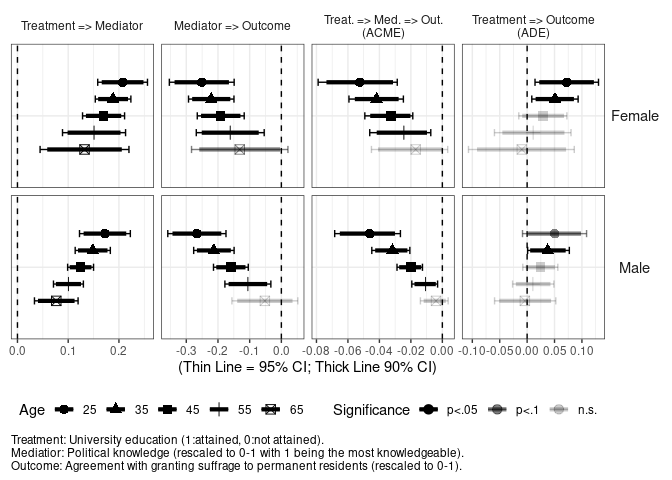
\includegraphics{analysis_4_mediation_matchednoL_v5_files/figure-latex/unnamed-chunk-21-1.pdf}

\begin{Shaded}
\begin{Highlighting}[]
\KeywordTok{ggsave}\NormalTok{(}\KeywordTok{paste0}\NormalTok{(projdir,}\StringTok{"/out/mediationplot_knowledge_matchednoL_v5.png"}\NormalTok{),p,}\DataTypeTok{width=}\DecValTok{8}\NormalTok{,}\DataTypeTok{height=}\DecValTok{5}\NormalTok{)}
\end{Highlighting}
\end{Shaded}

\begin{verbatim}
## Warning: position_dodge requires non-overlapping x intervals

## Warning: position_dodge requires non-overlapping x intervals

## Warning: position_dodge requires non-overlapping x intervals

## Warning: position_dodge requires non-overlapping x intervals

## Warning: position_dodge requires non-overlapping x intervals

## Warning: position_dodge requires non-overlapping x intervals

## Warning: position_dodge requires non-overlapping x intervals

## Warning: position_dodge requires non-overlapping x intervals
\end{verbatim}

\begin{Shaded}
\begin{Highlighting}[]
\KeywordTok{require}\NormalTok{(ggplot2)}
\NormalTok{p <-}\StringTok{ }\KeywordTok{ggplot}\NormalTok{(coefdt[coefdt}\OperatorTok{$}\NormalTok{med}\OperatorTok{==}\StringTok{"knowledge"} \OperatorTok{&}\StringTok{ }\NormalTok{coefdt}\OperatorTok{$}\NormalTok{mod}\OperatorTok{!=}\StringTok{"Treatment => Outcome}\CharTok{\textbackslash{}n}\StringTok{(ADE)"}\NormalTok{,], }\KeywordTok{aes}\NormalTok{(}\DataTypeTok{x=}\NormalTok{gender, }\DataTypeTok{y=}\NormalTok{est)) }\OperatorTok{+}
\StringTok{  }\KeywordTok{geom_hline}\NormalTok{(}\KeywordTok{aes}\NormalTok{(}\DataTypeTok{yintercept=}\DecValTok{0}\NormalTok{), }\DataTypeTok{linetype=}\DecValTok{2}\NormalTok{) }\OperatorTok{+}
\StringTok{  }\KeywordTok{geom_errorbar}\NormalTok{(}\KeywordTok{aes}\NormalTok{(}\DataTypeTok{ymin=}\NormalTok{lci95,}\DataTypeTok{ymax=}\NormalTok{uci95,}\DataTypeTok{colour=}\KeywordTok{as.factor}\NormalTok{(age), }\DataTypeTok{alpha=}\NormalTok{pstar), }
                \DataTypeTok{position=}\KeywordTok{position_dodge}\NormalTok{(}\DataTypeTok{width=}\OperatorTok{-}\FloatTok{0.7}\NormalTok{), }\DataTypeTok{size=}\FloatTok{0.5}\NormalTok{, }\DataTypeTok{width=}\FloatTok{0.3}\NormalTok{) }\OperatorTok{+}
\StringTok{  }\KeywordTok{geom_errorbar}\NormalTok{(}\KeywordTok{aes}\NormalTok{(}\DataTypeTok{ymin=}\NormalTok{lci90,}\DataTypeTok{ymax=}\NormalTok{uci90,}\DataTypeTok{colour=}\KeywordTok{as.factor}\NormalTok{(age), }\DataTypeTok{alpha=}\NormalTok{pstar),}
                \DataTypeTok{position=}\KeywordTok{position_dodge}\NormalTok{(}\DataTypeTok{width=}\OperatorTok{-}\FloatTok{0.7}\NormalTok{), }\DataTypeTok{size=}\FloatTok{1.5}\NormalTok{, }\DataTypeTok{width=}\FloatTok{0.0}\NormalTok{) }\OperatorTok{+}
\StringTok{  }\KeywordTok{geom_point}\NormalTok{(}\KeywordTok{aes}\NormalTok{(}\DataTypeTok{shape=}\KeywordTok{as.factor}\NormalTok{(age), }\DataTypeTok{colour=}\KeywordTok{as.factor}\NormalTok{(age), }\DataTypeTok{alpha=}\NormalTok{pstar),}
             \DataTypeTok{position=}\KeywordTok{position_dodge}\NormalTok{(}\DataTypeTok{width=}\OperatorTok{-}\FloatTok{0.7}\NormalTok{), }\DataTypeTok{size=}\DecValTok{3}\NormalTok{) }\OperatorTok{+}
\StringTok{  }\KeywordTok{facet_grid}\NormalTok{(gender }\OperatorTok{~}\StringTok{ }\NormalTok{mod, }\DataTypeTok{scales =} \StringTok{"free"}\NormalTok{) }\OperatorTok{+}
\StringTok{  }\KeywordTok{scale_alpha_manual}\NormalTok{(}\DataTypeTok{name=}\StringTok{"Significance"}\NormalTok{,}\DataTypeTok{values=}\KeywordTok{c}\NormalTok{(}\DecValTok{1}\NormalTok{,}\FloatTok{0.5}\NormalTok{,}\FloatTok{0.2}\NormalTok{), }\DataTypeTok{drop=}\OtherTok{FALSE}\NormalTok{) }\OperatorTok{+}
\StringTok{  }\KeywordTok{scale_shape_discrete}\NormalTok{(}\DataTypeTok{name=}\StringTok{"Age"}\NormalTok{) }\OperatorTok{+}
\StringTok{  }\KeywordTok{scale_color_manual}\NormalTok{(}\DataTypeTok{name=}\StringTok{"Age"}\NormalTok{,}\DataTypeTok{values=}\KeywordTok{rep}\NormalTok{(}\StringTok{"black"}\NormalTok{, }\DecValTok{5}\NormalTok{)) }\OperatorTok{+}
\StringTok{  }\KeywordTok{ylab}\NormalTok{(}\StringTok{"(Thin Line = 95% CI; Thick Line 90% CI)"}\NormalTok{) }\OperatorTok{+}
\StringTok{  }\KeywordTok{xlab}\NormalTok{(}\OtherTok{NULL}\NormalTok{) }\OperatorTok{+}
\StringTok{  }\KeywordTok{labs}\NormalTok{(}\DataTypeTok{caption=}\StringTok{"Treatment: University education (1:attained, 0:not attained). }\CharTok{\textbackslash{}n}\StringTok{Mediatior: Political knowledge (rescaled to 0-1 with 1 being the most knowledgeable).}\CharTok{\textbackslash{}n}\StringTok{Outcome: Agreement with granting suffrage to permanent residents (rescaled to 0-1)."}\NormalTok{) }\OperatorTok{+}
\StringTok{  }\KeywordTok{coord_flip}\NormalTok{() }\OperatorTok{+}\StringTok{ }\KeywordTok{theme_bw}\NormalTok{() }\OperatorTok{+}
\StringTok{  }\KeywordTok{theme}\NormalTok{(}\DataTypeTok{legend.position =} \StringTok{"bottom"}\NormalTok{,}
        \DataTypeTok{strip.text.x =} \KeywordTok{element_text}\NormalTok{(}\DataTypeTok{size=}\DecValTok{9}\NormalTok{),}
        \DataTypeTok{strip.text.y =} \KeywordTok{element_text}\NormalTok{(}\DataTypeTok{angle=}\DecValTok{0}\NormalTok{,}\DataTypeTok{size=}\DecValTok{11}\NormalTok{),}
        \DataTypeTok{strip.background =} \KeywordTok{element_rect}\NormalTok{(}\DataTypeTok{fill=}\OtherTok{NA}\NormalTok{,}\DataTypeTok{color=}\OtherTok{NA}\NormalTok{),}
        \DataTypeTok{plot.caption =} \KeywordTok{element_text}\NormalTok{(}\DataTypeTok{hjust=}\DecValTok{0}\NormalTok{),}
        \DataTypeTok{plot.subtitle =} \KeywordTok{element_text}\NormalTok{(}\DataTypeTok{hjust=}\FloatTok{0.5}\NormalTok{),}
        \DataTypeTok{axis.text.y =} \KeywordTok{element_blank}\NormalTok{(),}
        \DataTypeTok{axis.ticks.y =} \KeywordTok{element_blank}\NormalTok{())}
\NormalTok{p}
\end{Highlighting}
\end{Shaded}

\begin{verbatim}
## Warning: position_dodge requires non-overlapping x intervals

## Warning: position_dodge requires non-overlapping x intervals

## Warning: position_dodge requires non-overlapping x intervals

## Warning: position_dodge requires non-overlapping x intervals

## Warning: position_dodge requires non-overlapping x intervals

## Warning: position_dodge requires non-overlapping x intervals
\end{verbatim}

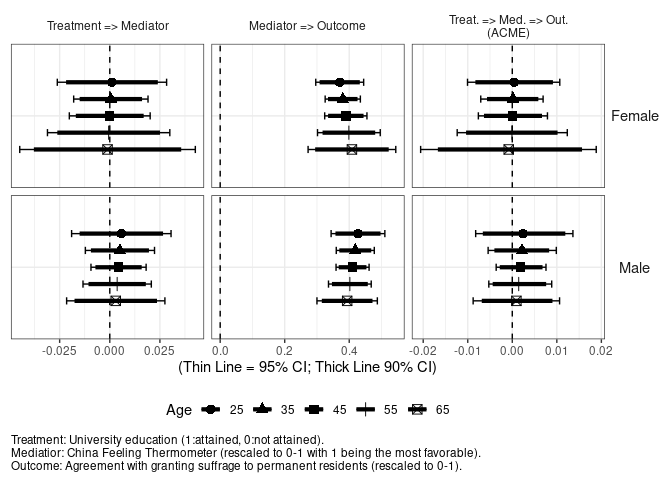
\includegraphics{analysis_4_mediation_matchednoL_v5_files/figure-latex/unnamed-chunk-21-2.pdf}

\begin{Shaded}
\begin{Highlighting}[]
\KeywordTok{ggsave}\NormalTok{(}\KeywordTok{paste0}\NormalTok{(projdir,}\StringTok{"/out/mediationplot2_knowledge_matchednoL_v5.png"}\NormalTok{),p,}\DataTypeTok{width=}\DecValTok{8}\NormalTok{,}\DataTypeTok{height=}\DecValTok{5}\NormalTok{)}
\end{Highlighting}
\end{Shaded}

\begin{verbatim}
## Warning: position_dodge requires non-overlapping x intervals

## Warning: position_dodge requires non-overlapping x intervals

## Warning: position_dodge requires non-overlapping x intervals

## Warning: position_dodge requires non-overlapping x intervals

## Warning: position_dodge requires non-overlapping x intervals

## Warning: position_dodge requires non-overlapping x intervals
\end{verbatim}

\hypertarget{plotting-for-ideology}{%
\subsection{Plotting for ideology}\label{plotting-for-ideology}}

\begin{Shaded}
\begin{Highlighting}[]
\KeywordTok{require}\NormalTok{(ggplot2)}
\NormalTok{p <-}\StringTok{ }\KeywordTok{ggplot}\NormalTok{(coefdt[coefdt}\OperatorTok{$}\NormalTok{med}\OperatorTok{==}\StringTok{"ideology"}\NormalTok{,], }\KeywordTok{aes}\NormalTok{(}\DataTypeTok{x=}\NormalTok{gender, }\DataTypeTok{y=}\NormalTok{est)) }\OperatorTok{+}
\StringTok{  }\KeywordTok{geom_hline}\NormalTok{(}\KeywordTok{aes}\NormalTok{(}\DataTypeTok{yintercept=}\DecValTok{0}\NormalTok{), }\DataTypeTok{linetype=}\DecValTok{2}\NormalTok{) }\OperatorTok{+}
\StringTok{  }\KeywordTok{geom_errorbar}\NormalTok{(}\KeywordTok{aes}\NormalTok{(}\DataTypeTok{ymin=}\NormalTok{lci95,}\DataTypeTok{ymax=}\NormalTok{uci95,}\DataTypeTok{colour=}\KeywordTok{as.factor}\NormalTok{(age), }\DataTypeTok{alpha=}\NormalTok{pstar), }
                \DataTypeTok{position=}\KeywordTok{position_dodge}\NormalTok{(}\DataTypeTok{width=}\OperatorTok{-}\FloatTok{0.7}\NormalTok{), }\DataTypeTok{size=}\FloatTok{0.5}\NormalTok{, }\DataTypeTok{width=}\FloatTok{0.3}\NormalTok{) }\OperatorTok{+}
\StringTok{  }\KeywordTok{geom_errorbar}\NormalTok{(}\KeywordTok{aes}\NormalTok{(}\DataTypeTok{ymin=}\NormalTok{lci90,}\DataTypeTok{ymax=}\NormalTok{uci90,}\DataTypeTok{colour=}\KeywordTok{as.factor}\NormalTok{(age), }\DataTypeTok{alpha=}\NormalTok{pstar),}
                \DataTypeTok{position=}\KeywordTok{position_dodge}\NormalTok{(}\DataTypeTok{width=}\OperatorTok{-}\FloatTok{0.7}\NormalTok{), }\DataTypeTok{size=}\FloatTok{1.5}\NormalTok{, }\DataTypeTok{width=}\FloatTok{0.0}\NormalTok{) }\OperatorTok{+}
\StringTok{  }\KeywordTok{geom_point}\NormalTok{(}\KeywordTok{aes}\NormalTok{(}\DataTypeTok{shape=}\KeywordTok{as.factor}\NormalTok{(age), }\DataTypeTok{colour=}\KeywordTok{as.factor}\NormalTok{(age), }\DataTypeTok{alpha=}\NormalTok{pstar),}
             \DataTypeTok{position=}\KeywordTok{position_dodge}\NormalTok{(}\DataTypeTok{width=}\OperatorTok{-}\FloatTok{0.7}\NormalTok{), }\DataTypeTok{size=}\DecValTok{3}\NormalTok{) }\OperatorTok{+}
\StringTok{  }\KeywordTok{facet_grid}\NormalTok{(gender }\OperatorTok{~}\StringTok{ }\NormalTok{mod, }\DataTypeTok{scales =} \StringTok{"free"}\NormalTok{) }\OperatorTok{+}
\StringTok{  }\KeywordTok{scale_alpha_manual}\NormalTok{(}\DataTypeTok{name=}\StringTok{"Significance"}\NormalTok{,}\DataTypeTok{values=}\KeywordTok{c}\NormalTok{(}\DecValTok{1}\NormalTok{,}\FloatTok{0.5}\NormalTok{,}\FloatTok{0.2}\NormalTok{), }\DataTypeTok{drop=}\OtherTok{FALSE}\NormalTok{) }\OperatorTok{+}
\StringTok{  }\KeywordTok{scale_shape_discrete}\NormalTok{(}\DataTypeTok{name=}\StringTok{"Age"}\NormalTok{) }\OperatorTok{+}
\StringTok{  }\KeywordTok{scale_color_manual}\NormalTok{(}\DataTypeTok{name=}\StringTok{"Age"}\NormalTok{,}\DataTypeTok{values=}\KeywordTok{rep}\NormalTok{(}\StringTok{"black"}\NormalTok{, }\DecValTok{5}\NormalTok{)) }\OperatorTok{+}
\StringTok{  }\KeywordTok{ylab}\NormalTok{(}\StringTok{"(Thin Line = 95% CI; Thick Line 90% CI)"}\NormalTok{) }\OperatorTok{+}
\StringTok{  }\KeywordTok{xlab}\NormalTok{(}\OtherTok{NULL}\NormalTok{) }\OperatorTok{+}
\StringTok{  }\KeywordTok{labs}\NormalTok{(}\DataTypeTok{caption=}\StringTok{"Treatment: University education (1:attained, 0:not attained). }\CharTok{\textbackslash{}n}\StringTok{Mediatior: Political ideology (rescaled to 0-1 with 1 being the most conservative).}\CharTok{\textbackslash{}n}\StringTok{Outcome: Agreement with granting suffrage to permanent residents (rescaled to 0-1)."}\NormalTok{) }\OperatorTok{+}
\StringTok{  }\KeywordTok{coord_flip}\NormalTok{() }\OperatorTok{+}\StringTok{ }\KeywordTok{theme_bw}\NormalTok{() }\OperatorTok{+}
\StringTok{  }\KeywordTok{theme}\NormalTok{(}\DataTypeTok{legend.position =} \StringTok{"bottom"}\NormalTok{,}
        \DataTypeTok{strip.text.x =} \KeywordTok{element_text}\NormalTok{(}\DataTypeTok{size=}\DecValTok{9}\NormalTok{),}
        \DataTypeTok{strip.text.y =} \KeywordTok{element_text}\NormalTok{(}\DataTypeTok{angle=}\DecValTok{0}\NormalTok{,}\DataTypeTok{size=}\DecValTok{11}\NormalTok{),}
        \DataTypeTok{strip.background =} \KeywordTok{element_rect}\NormalTok{(}\DataTypeTok{fill=}\OtherTok{NA}\NormalTok{,}\DataTypeTok{color=}\OtherTok{NA}\NormalTok{),}
        \DataTypeTok{plot.caption =} \KeywordTok{element_text}\NormalTok{(}\DataTypeTok{hjust=}\DecValTok{0}\NormalTok{),}
        \DataTypeTok{plot.subtitle =} \KeywordTok{element_text}\NormalTok{(}\DataTypeTok{hjust=}\FloatTok{0.5}\NormalTok{),}
        \DataTypeTok{axis.text.y =} \KeywordTok{element_blank}\NormalTok{(),}
        \DataTypeTok{axis.ticks.y =} \KeywordTok{element_blank}\NormalTok{())}
\NormalTok{p}
\end{Highlighting}
\end{Shaded}

\begin{verbatim}
## Warning: position_dodge requires non-overlapping x intervals

## Warning: position_dodge requires non-overlapping x intervals

## Warning: position_dodge requires non-overlapping x intervals

## Warning: position_dodge requires non-overlapping x intervals

## Warning: position_dodge requires non-overlapping x intervals

## Warning: position_dodge requires non-overlapping x intervals

## Warning: position_dodge requires non-overlapping x intervals

## Warning: position_dodge requires non-overlapping x intervals
\end{verbatim}

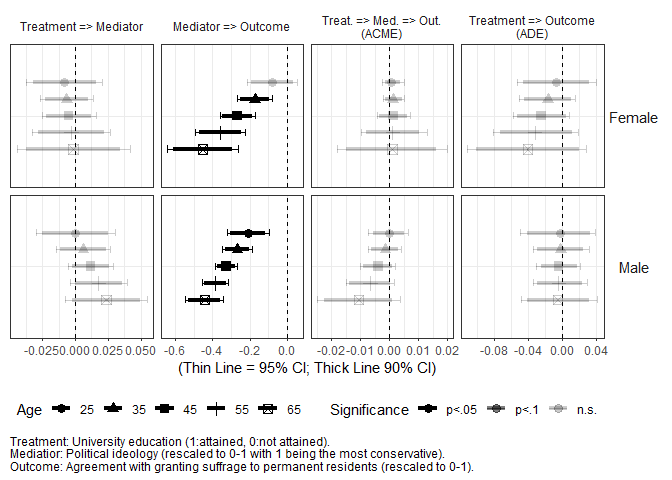
\includegraphics{analysis_4_mediation_matchednoL_v5_files/figure-latex/unnamed-chunk-22-1.pdf}

\begin{Shaded}
\begin{Highlighting}[]
\KeywordTok{ggsave}\NormalTok{(}\KeywordTok{paste0}\NormalTok{(projdir,}\StringTok{"/out/mediationplot_ideology_matchednoL_v5.png"}\NormalTok{),p,}\DataTypeTok{width=}\DecValTok{8}\NormalTok{,}\DataTypeTok{height=}\DecValTok{5}\NormalTok{)}
\end{Highlighting}
\end{Shaded}

\begin{verbatim}
## Warning: position_dodge requires non-overlapping x intervals

## Warning: position_dodge requires non-overlapping x intervals

## Warning: position_dodge requires non-overlapping x intervals

## Warning: position_dodge requires non-overlapping x intervals

## Warning: position_dodge requires non-overlapping x intervals

## Warning: position_dodge requires non-overlapping x intervals

## Warning: position_dodge requires non-overlapping x intervals

## Warning: position_dodge requires non-overlapping x intervals
\end{verbatim}

\begin{Shaded}
\begin{Highlighting}[]
\KeywordTok{require}\NormalTok{(ggplot2)}
\NormalTok{p <-}\StringTok{ }\KeywordTok{ggplot}\NormalTok{(coefdt[coefdt}\OperatorTok{$}\NormalTok{med}\OperatorTok{==}\StringTok{"ideology"} \OperatorTok{&}\StringTok{ }\NormalTok{coefdt}\OperatorTok{$}\NormalTok{mod}\OperatorTok{!=}\StringTok{"Treatment => Outcome}\CharTok{\textbackslash{}n}\StringTok{(ADE)"}\NormalTok{,], }\KeywordTok{aes}\NormalTok{(}\DataTypeTok{x=}\NormalTok{gender, }\DataTypeTok{y=}\NormalTok{est)) }\OperatorTok{+}
\StringTok{  }\KeywordTok{geom_hline}\NormalTok{(}\KeywordTok{aes}\NormalTok{(}\DataTypeTok{yintercept=}\DecValTok{0}\NormalTok{), }\DataTypeTok{linetype=}\DecValTok{2}\NormalTok{) }\OperatorTok{+}
\StringTok{  }\KeywordTok{geom_errorbar}\NormalTok{(}\KeywordTok{aes}\NormalTok{(}\DataTypeTok{ymin=}\NormalTok{lci95,}\DataTypeTok{ymax=}\NormalTok{uci95,}\DataTypeTok{colour=}\KeywordTok{as.factor}\NormalTok{(age), }\DataTypeTok{alpha=}\NormalTok{pstar), }
                \DataTypeTok{position=}\KeywordTok{position_dodge}\NormalTok{(}\DataTypeTok{width=}\OperatorTok{-}\FloatTok{0.7}\NormalTok{), }\DataTypeTok{size=}\FloatTok{0.5}\NormalTok{, }\DataTypeTok{width=}\FloatTok{0.3}\NormalTok{) }\OperatorTok{+}
\StringTok{  }\KeywordTok{geom_errorbar}\NormalTok{(}\KeywordTok{aes}\NormalTok{(}\DataTypeTok{ymin=}\NormalTok{lci90,}\DataTypeTok{ymax=}\NormalTok{uci90,}\DataTypeTok{colour=}\KeywordTok{as.factor}\NormalTok{(age), }\DataTypeTok{alpha=}\NormalTok{pstar),}
                \DataTypeTok{position=}\KeywordTok{position_dodge}\NormalTok{(}\DataTypeTok{width=}\OperatorTok{-}\FloatTok{0.7}\NormalTok{), }\DataTypeTok{size=}\FloatTok{1.5}\NormalTok{, }\DataTypeTok{width=}\FloatTok{0.0}\NormalTok{) }\OperatorTok{+}
\StringTok{  }\KeywordTok{geom_point}\NormalTok{(}\KeywordTok{aes}\NormalTok{(}\DataTypeTok{shape=}\KeywordTok{as.factor}\NormalTok{(age), }\DataTypeTok{colour=}\KeywordTok{as.factor}\NormalTok{(age), }\DataTypeTok{alpha=}\NormalTok{pstar),}
             \DataTypeTok{position=}\KeywordTok{position_dodge}\NormalTok{(}\DataTypeTok{width=}\OperatorTok{-}\FloatTok{0.7}\NormalTok{), }\DataTypeTok{size=}\DecValTok{3}\NormalTok{) }\OperatorTok{+}
\StringTok{  }\KeywordTok{facet_grid}\NormalTok{(gender }\OperatorTok{~}\StringTok{ }\NormalTok{mod, }\DataTypeTok{scales =} \StringTok{"free"}\NormalTok{) }\OperatorTok{+}
\StringTok{  }\KeywordTok{scale_alpha_manual}\NormalTok{(}\DataTypeTok{name=}\StringTok{"Significance"}\NormalTok{,}\DataTypeTok{values=}\KeywordTok{c}\NormalTok{(}\DecValTok{1}\NormalTok{,}\FloatTok{0.5}\NormalTok{,}\FloatTok{0.2}\NormalTok{), }\DataTypeTok{drop=}\OtherTok{FALSE}\NormalTok{) }\OperatorTok{+}
\StringTok{  }\KeywordTok{scale_shape_discrete}\NormalTok{(}\DataTypeTok{name=}\StringTok{"Age"}\NormalTok{) }\OperatorTok{+}
\StringTok{  }\KeywordTok{scale_color_manual}\NormalTok{(}\DataTypeTok{name=}\StringTok{"Age"}\NormalTok{,}\DataTypeTok{values=}\KeywordTok{rep}\NormalTok{(}\StringTok{"black"}\NormalTok{, }\DecValTok{5}\NormalTok{)) }\OperatorTok{+}
\StringTok{  }\KeywordTok{ylab}\NormalTok{(}\StringTok{"(Thin Line = 95% CI; Thick Line 90% CI)"}\NormalTok{) }\OperatorTok{+}
\StringTok{  }\KeywordTok{xlab}\NormalTok{(}\OtherTok{NULL}\NormalTok{) }\OperatorTok{+}
\StringTok{  }\KeywordTok{labs}\NormalTok{(}\DataTypeTok{caption=}\StringTok{"Treatment: University education (1:attained, 0:not attained). }\CharTok{\textbackslash{}n}\StringTok{Mediatior: Political ideology (rescaled to 0-1 with 1 being the most conservative).}\CharTok{\textbackslash{}n}\StringTok{Outcome: Agreement with granting suffrage to permanent residents (rescaled to 0-1)."}\NormalTok{) }\OperatorTok{+}
\StringTok{  }\KeywordTok{coord_flip}\NormalTok{() }\OperatorTok{+}\StringTok{ }\KeywordTok{theme_bw}\NormalTok{() }\OperatorTok{+}
\StringTok{  }\KeywordTok{theme}\NormalTok{(}\DataTypeTok{legend.position =} \StringTok{"bottom"}\NormalTok{,}
        \DataTypeTok{strip.text.x =} \KeywordTok{element_text}\NormalTok{(}\DataTypeTok{size=}\DecValTok{9}\NormalTok{),}
        \DataTypeTok{strip.text.y =} \KeywordTok{element_text}\NormalTok{(}\DataTypeTok{angle=}\DecValTok{0}\NormalTok{,}\DataTypeTok{size=}\DecValTok{11}\NormalTok{),}
        \DataTypeTok{strip.background =} \KeywordTok{element_rect}\NormalTok{(}\DataTypeTok{fill=}\OtherTok{NA}\NormalTok{,}\DataTypeTok{color=}\OtherTok{NA}\NormalTok{),}
        \DataTypeTok{plot.caption =} \KeywordTok{element_text}\NormalTok{(}\DataTypeTok{hjust=}\DecValTok{0}\NormalTok{),}
        \DataTypeTok{plot.subtitle =} \KeywordTok{element_text}\NormalTok{(}\DataTypeTok{hjust=}\FloatTok{0.5}\NormalTok{),}
        \DataTypeTok{axis.text.y =} \KeywordTok{element_blank}\NormalTok{(),}
        \DataTypeTok{axis.ticks.y =} \KeywordTok{element_blank}\NormalTok{())}
\NormalTok{p}
\end{Highlighting}
\end{Shaded}

\begin{verbatim}
## Warning: position_dodge requires non-overlapping x intervals

## Warning: position_dodge requires non-overlapping x intervals

## Warning: position_dodge requires non-overlapping x intervals

## Warning: position_dodge requires non-overlapping x intervals

## Warning: position_dodge requires non-overlapping x intervals

## Warning: position_dodge requires non-overlapping x intervals
\end{verbatim}

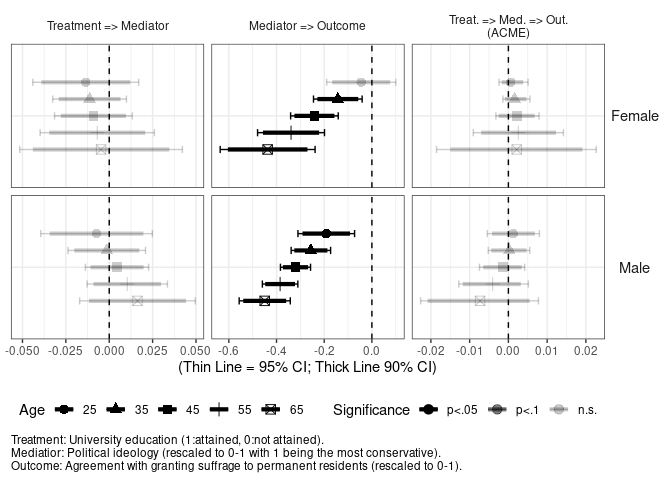
\includegraphics{analysis_4_mediation_matchednoL_v5_files/figure-latex/unnamed-chunk-22-2.pdf}

\begin{Shaded}
\begin{Highlighting}[]
\KeywordTok{ggsave}\NormalTok{(}\KeywordTok{paste0}\NormalTok{(projdir,}\StringTok{"/out/mediationplot2_ideology_matchednoL_v5.png"}\NormalTok{),p,}\DataTypeTok{width=}\DecValTok{8}\NormalTok{,}\DataTypeTok{height=}\DecValTok{5}\NormalTok{)}
\end{Highlighting}
\end{Shaded}

\begin{verbatim}
## Warning: position_dodge requires non-overlapping x intervals

## Warning: position_dodge requires non-overlapping x intervals

## Warning: position_dodge requires non-overlapping x intervals

## Warning: position_dodge requires non-overlapping x intervals

## Warning: position_dodge requires non-overlapping x intervals

## Warning: position_dodge requires non-overlapping x intervals
\end{verbatim}

\hypertarget{plotting-for-ldpdpjft}{%
\subsection{Plotting for ldpdpjft}\label{plotting-for-ldpdpjft}}

\begin{Shaded}
\begin{Highlighting}[]
\KeywordTok{require}\NormalTok{(ggplot2)}
\NormalTok{p <-}\StringTok{ }\KeywordTok{ggplot}\NormalTok{(coefdt[coefdt}\OperatorTok{$}\NormalTok{med}\OperatorTok{==}\StringTok{"ldpdpjft"}\NormalTok{,], }\KeywordTok{aes}\NormalTok{(}\DataTypeTok{x=}\NormalTok{gender, }\DataTypeTok{y=}\NormalTok{est)) }\OperatorTok{+}
\StringTok{  }\KeywordTok{geom_hline}\NormalTok{(}\KeywordTok{aes}\NormalTok{(}\DataTypeTok{yintercept=}\DecValTok{0}\NormalTok{), }\DataTypeTok{linetype=}\DecValTok{2}\NormalTok{) }\OperatorTok{+}
\StringTok{  }\KeywordTok{geom_errorbar}\NormalTok{(}\KeywordTok{aes}\NormalTok{(}\DataTypeTok{ymin=}\NormalTok{lci95,}\DataTypeTok{ymax=}\NormalTok{uci95,}\DataTypeTok{colour=}\KeywordTok{as.factor}\NormalTok{(age), }\DataTypeTok{alpha=}\NormalTok{pstar), }
                \DataTypeTok{position=}\KeywordTok{position_dodge}\NormalTok{(}\DataTypeTok{width=}\OperatorTok{-}\FloatTok{0.7}\NormalTok{), }\DataTypeTok{size=}\FloatTok{0.5}\NormalTok{, }\DataTypeTok{width=}\FloatTok{0.3}\NormalTok{) }\OperatorTok{+}
\StringTok{  }\KeywordTok{geom_errorbar}\NormalTok{(}\KeywordTok{aes}\NormalTok{(}\DataTypeTok{ymin=}\NormalTok{lci90,}\DataTypeTok{ymax=}\NormalTok{uci90,}\DataTypeTok{colour=}\KeywordTok{as.factor}\NormalTok{(age), }\DataTypeTok{alpha=}\NormalTok{pstar),}
                \DataTypeTok{position=}\KeywordTok{position_dodge}\NormalTok{(}\DataTypeTok{width=}\OperatorTok{-}\FloatTok{0.7}\NormalTok{), }\DataTypeTok{size=}\FloatTok{1.5}\NormalTok{, }\DataTypeTok{width=}\FloatTok{0.0}\NormalTok{) }\OperatorTok{+}
\StringTok{  }\KeywordTok{geom_point}\NormalTok{(}\KeywordTok{aes}\NormalTok{(}\DataTypeTok{shape=}\KeywordTok{as.factor}\NormalTok{(age), }\DataTypeTok{colour=}\KeywordTok{as.factor}\NormalTok{(age), }\DataTypeTok{alpha=}\NormalTok{pstar),}
             \DataTypeTok{position=}\KeywordTok{position_dodge}\NormalTok{(}\DataTypeTok{width=}\OperatorTok{-}\FloatTok{0.7}\NormalTok{), }\DataTypeTok{size=}\DecValTok{3}\NormalTok{) }\OperatorTok{+}
\StringTok{  }\KeywordTok{facet_grid}\NormalTok{(gender }\OperatorTok{~}\StringTok{ }\NormalTok{mod, }\DataTypeTok{scales =} \StringTok{"free"}\NormalTok{) }\OperatorTok{+}
\StringTok{  }\KeywordTok{scale_alpha_manual}\NormalTok{(}\DataTypeTok{name=}\StringTok{"Significance"}\NormalTok{,}\DataTypeTok{values=}\KeywordTok{c}\NormalTok{(}\DecValTok{1}\NormalTok{,}\FloatTok{0.5}\NormalTok{,}\FloatTok{0.2}\NormalTok{), }\DataTypeTok{drop=}\OtherTok{FALSE}\NormalTok{) }\OperatorTok{+}
\StringTok{  }\KeywordTok{scale_shape_discrete}\NormalTok{(}\DataTypeTok{name=}\StringTok{"Age"}\NormalTok{) }\OperatorTok{+}
\StringTok{  }\KeywordTok{scale_color_manual}\NormalTok{(}\DataTypeTok{name=}\StringTok{"Age"}\NormalTok{,}\DataTypeTok{values=}\KeywordTok{rep}\NormalTok{(}\StringTok{"black"}\NormalTok{, }\DecValTok{5}\NormalTok{)) }\OperatorTok{+}
\StringTok{  }\KeywordTok{ylab}\NormalTok{(}\StringTok{"(Thin Line = 95% CI; Thick Line 90% CI)"}\NormalTok{) }\OperatorTok{+}
\StringTok{  }\KeywordTok{xlab}\NormalTok{(}\OtherTok{NULL}\NormalTok{) }\OperatorTok{+}
\StringTok{  }\KeywordTok{labs}\NormalTok{(}\DataTypeTok{caption=}\StringTok{"Treatment: University education (1:attained, 0:not attained). }\CharTok{\textbackslash{}n}\StringTok{Mediatior: LDP - DPJ Feeling Thermometer (rescaled to 0-1).}\CharTok{\textbackslash{}n}\StringTok{Outcome: Agreement with granting suffrage to permanent residents (rescaled to 0-1)."}\NormalTok{) }\OperatorTok{+}
\StringTok{  }\KeywordTok{coord_flip}\NormalTok{() }\OperatorTok{+}\StringTok{ }\KeywordTok{theme_bw}\NormalTok{() }\OperatorTok{+}
\StringTok{  }\KeywordTok{theme}\NormalTok{(}\DataTypeTok{legend.position =} \StringTok{"bottom"}\NormalTok{,}
        \DataTypeTok{strip.text.x =} \KeywordTok{element_text}\NormalTok{(}\DataTypeTok{size=}\DecValTok{9}\NormalTok{),}
        \DataTypeTok{strip.text.y =} \KeywordTok{element_text}\NormalTok{(}\DataTypeTok{angle=}\DecValTok{0}\NormalTok{,}\DataTypeTok{size=}\DecValTok{11}\NormalTok{),}
        \DataTypeTok{strip.background =} \KeywordTok{element_rect}\NormalTok{(}\DataTypeTok{fill=}\OtherTok{NA}\NormalTok{,}\DataTypeTok{color=}\OtherTok{NA}\NormalTok{),}
        \DataTypeTok{plot.caption =} \KeywordTok{element_text}\NormalTok{(}\DataTypeTok{hjust=}\DecValTok{0}\NormalTok{),}
        \DataTypeTok{plot.subtitle =} \KeywordTok{element_text}\NormalTok{(}\DataTypeTok{hjust=}\FloatTok{0.5}\NormalTok{),}
        \DataTypeTok{axis.text.y =} \KeywordTok{element_blank}\NormalTok{(),}
        \DataTypeTok{axis.ticks.y =} \KeywordTok{element_blank}\NormalTok{())}
\NormalTok{p}
\end{Highlighting}
\end{Shaded}

\begin{verbatim}
## Warning: position_dodge requires non-overlapping x intervals

## Warning: position_dodge requires non-overlapping x intervals

## Warning: position_dodge requires non-overlapping x intervals

## Warning: position_dodge requires non-overlapping x intervals

## Warning: position_dodge requires non-overlapping x intervals

## Warning: position_dodge requires non-overlapping x intervals

## Warning: position_dodge requires non-overlapping x intervals

## Warning: position_dodge requires non-overlapping x intervals
\end{verbatim}

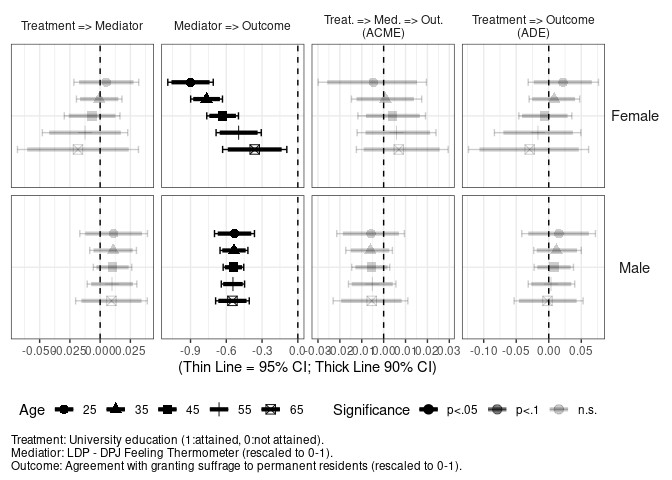
\includegraphics{analysis_4_mediation_matchednoL_v5_files/figure-latex/unnamed-chunk-23-1.pdf}

\begin{Shaded}
\begin{Highlighting}[]
\KeywordTok{ggsave}\NormalTok{(}\KeywordTok{paste0}\NormalTok{(projdir,}\StringTok{"/out/mediationplot_ldpdpjft_matchednoL_v5.png"}\NormalTok{),p,}\DataTypeTok{width=}\DecValTok{8}\NormalTok{,}\DataTypeTok{height=}\DecValTok{5}\NormalTok{)}
\end{Highlighting}
\end{Shaded}

\begin{verbatim}
## Warning: position_dodge requires non-overlapping x intervals

## Warning: position_dodge requires non-overlapping x intervals

## Warning: position_dodge requires non-overlapping x intervals

## Warning: position_dodge requires non-overlapping x intervals

## Warning: position_dodge requires non-overlapping x intervals

## Warning: position_dodge requires non-overlapping x intervals

## Warning: position_dodge requires non-overlapping x intervals

## Warning: position_dodge requires non-overlapping x intervals
\end{verbatim}

\begin{Shaded}
\begin{Highlighting}[]
\KeywordTok{require}\NormalTok{(ggplot2)}
\NormalTok{p <-}\StringTok{ }\KeywordTok{ggplot}\NormalTok{(coefdt[coefdt}\OperatorTok{$}\NormalTok{med}\OperatorTok{==}\StringTok{"ldpdpjft"} \OperatorTok{&}\StringTok{ }\NormalTok{coefdt}\OperatorTok{$}\NormalTok{mod}\OperatorTok{!=}\StringTok{"Treatment => Outcome}\CharTok{\textbackslash{}n}\StringTok{(ADE)"}\NormalTok{,], }\KeywordTok{aes}\NormalTok{(}\DataTypeTok{x=}\NormalTok{gender, }\DataTypeTok{y=}\NormalTok{est)) }\OperatorTok{+}
\StringTok{  }\KeywordTok{geom_hline}\NormalTok{(}\KeywordTok{aes}\NormalTok{(}\DataTypeTok{yintercept=}\DecValTok{0}\NormalTok{), }\DataTypeTok{linetype=}\DecValTok{2}\NormalTok{) }\OperatorTok{+}
\StringTok{  }\KeywordTok{geom_errorbar}\NormalTok{(}\KeywordTok{aes}\NormalTok{(}\DataTypeTok{ymin=}\NormalTok{lci95,}\DataTypeTok{ymax=}\NormalTok{uci95,}\DataTypeTok{colour=}\KeywordTok{as.factor}\NormalTok{(age), }\DataTypeTok{alpha=}\NormalTok{pstar), }
                \DataTypeTok{position=}\KeywordTok{position_dodge}\NormalTok{(}\DataTypeTok{width=}\OperatorTok{-}\FloatTok{0.7}\NormalTok{), }\DataTypeTok{size=}\FloatTok{0.5}\NormalTok{, }\DataTypeTok{width=}\FloatTok{0.3}\NormalTok{) }\OperatorTok{+}
\StringTok{  }\KeywordTok{geom_errorbar}\NormalTok{(}\KeywordTok{aes}\NormalTok{(}\DataTypeTok{ymin=}\NormalTok{lci90,}\DataTypeTok{ymax=}\NormalTok{uci90,}\DataTypeTok{colour=}\KeywordTok{as.factor}\NormalTok{(age), }\DataTypeTok{alpha=}\NormalTok{pstar),}
                \DataTypeTok{position=}\KeywordTok{position_dodge}\NormalTok{(}\DataTypeTok{width=}\OperatorTok{-}\FloatTok{0.7}\NormalTok{), }\DataTypeTok{size=}\FloatTok{1.5}\NormalTok{, }\DataTypeTok{width=}\FloatTok{0.0}\NormalTok{) }\OperatorTok{+}
\StringTok{  }\KeywordTok{geom_point}\NormalTok{(}\KeywordTok{aes}\NormalTok{(}\DataTypeTok{shape=}\KeywordTok{as.factor}\NormalTok{(age), }\DataTypeTok{colour=}\KeywordTok{as.factor}\NormalTok{(age), }\DataTypeTok{alpha=}\NormalTok{pstar),}
             \DataTypeTok{position=}\KeywordTok{position_dodge}\NormalTok{(}\DataTypeTok{width=}\OperatorTok{-}\FloatTok{0.7}\NormalTok{), }\DataTypeTok{size=}\DecValTok{3}\NormalTok{) }\OperatorTok{+}
\StringTok{  }\KeywordTok{facet_grid}\NormalTok{(gender }\OperatorTok{~}\StringTok{ }\NormalTok{mod, }\DataTypeTok{scales =} \StringTok{"free"}\NormalTok{) }\OperatorTok{+}
\StringTok{  }\KeywordTok{scale_alpha_manual}\NormalTok{(}\DataTypeTok{name=}\StringTok{"Significance"}\NormalTok{,}\DataTypeTok{values=}\KeywordTok{c}\NormalTok{(}\DecValTok{1}\NormalTok{,}\FloatTok{0.5}\NormalTok{,}\FloatTok{0.2}\NormalTok{), }\DataTypeTok{drop=}\OtherTok{FALSE}\NormalTok{) }\OperatorTok{+}
\StringTok{  }\KeywordTok{scale_shape_discrete}\NormalTok{(}\DataTypeTok{name=}\StringTok{"Age"}\NormalTok{) }\OperatorTok{+}
\StringTok{  }\KeywordTok{scale_color_manual}\NormalTok{(}\DataTypeTok{name=}\StringTok{"Age"}\NormalTok{,}\DataTypeTok{values=}\KeywordTok{rep}\NormalTok{(}\StringTok{"black"}\NormalTok{, }\DecValTok{5}\NormalTok{)) }\OperatorTok{+}
\StringTok{  }\KeywordTok{ylab}\NormalTok{(}\StringTok{"(Thin Line = 95% CI; Thick Line 90% CI)"}\NormalTok{) }\OperatorTok{+}
\StringTok{  }\KeywordTok{xlab}\NormalTok{(}\OtherTok{NULL}\NormalTok{) }\OperatorTok{+}
\StringTok{  }\KeywordTok{labs}\NormalTok{(}\DataTypeTok{caption=}\StringTok{"Treatment: University education (1:attained, 0:not attained). }\CharTok{\textbackslash{}n}\StringTok{Mediatior: LDP - DPJ Feeling Thermometer (rescaled to 0-1).}\CharTok{\textbackslash{}n}\StringTok{Outcome: Agreement with granting suffrage to permanent residents (rescaled to 0-1)."}\NormalTok{) }\OperatorTok{+}
\StringTok{  }\KeywordTok{coord_flip}\NormalTok{() }\OperatorTok{+}\StringTok{ }\KeywordTok{theme_bw}\NormalTok{() }\OperatorTok{+}
\StringTok{  }\KeywordTok{theme}\NormalTok{(}\DataTypeTok{legend.position =} \StringTok{"bottom"}\NormalTok{,}
        \DataTypeTok{strip.text.x =} \KeywordTok{element_text}\NormalTok{(}\DataTypeTok{size=}\DecValTok{9}\NormalTok{),}
        \DataTypeTok{strip.text.y =} \KeywordTok{element_text}\NormalTok{(}\DataTypeTok{angle=}\DecValTok{0}\NormalTok{,}\DataTypeTok{size=}\DecValTok{11}\NormalTok{),}
        \DataTypeTok{strip.background =} \KeywordTok{element_rect}\NormalTok{(}\DataTypeTok{fill=}\OtherTok{NA}\NormalTok{,}\DataTypeTok{color=}\OtherTok{NA}\NormalTok{),}
        \DataTypeTok{plot.caption =} \KeywordTok{element_text}\NormalTok{(}\DataTypeTok{hjust=}\DecValTok{0}\NormalTok{),}
        \DataTypeTok{plot.subtitle =} \KeywordTok{element_text}\NormalTok{(}\DataTypeTok{hjust=}\FloatTok{0.5}\NormalTok{),}
        \DataTypeTok{axis.text.y =} \KeywordTok{element_blank}\NormalTok{(),}
        \DataTypeTok{axis.ticks.y =} \KeywordTok{element_blank}\NormalTok{())}
\NormalTok{p}
\end{Highlighting}
\end{Shaded}

\begin{verbatim}
## Warning: position_dodge requires non-overlapping x intervals

## Warning: position_dodge requires non-overlapping x intervals

## Warning: position_dodge requires non-overlapping x intervals

## Warning: position_dodge requires non-overlapping x intervals

## Warning: position_dodge requires non-overlapping x intervals

## Warning: position_dodge requires non-overlapping x intervals
\end{verbatim}

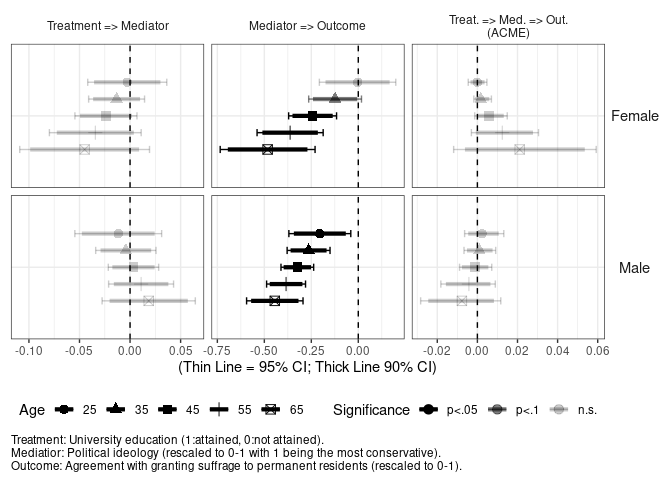
\includegraphics{analysis_4_mediation_matchednoL_v5_files/figure-latex/unnamed-chunk-23-2.pdf}

\begin{Shaded}
\begin{Highlighting}[]
\KeywordTok{ggsave}\NormalTok{(}\KeywordTok{paste0}\NormalTok{(projdir,}\StringTok{"/out/mediationplot2_ldpdpjft_matchednoL_v5.png"}\NormalTok{),p,}\DataTypeTok{width=}\DecValTok{8}\NormalTok{,}\DataTypeTok{height=}\DecValTok{5}\NormalTok{)}
\end{Highlighting}
\end{Shaded}

\begin{verbatim}
## Warning: position_dodge requires non-overlapping x intervals

## Warning: position_dodge requires non-overlapping x intervals

## Warning: position_dodge requires non-overlapping x intervals

## Warning: position_dodge requires non-overlapping x intervals

## Warning: position_dodge requires non-overlapping x intervals

## Warning: position_dodge requires non-overlapping x intervals
\end{verbatim}

\hypertarget{plotting-for-south-korea-feeling-thermometer}{%
\subsection{Plotting for South Korea Feeling
Thermometer}\label{plotting-for-south-korea-feeling-thermometer}}

\begin{Shaded}
\begin{Highlighting}[]
\KeywordTok{require}\NormalTok{(ggplot2)}
\NormalTok{p <-}\StringTok{ }\KeywordTok{ggplot}\NormalTok{(coefdt[coefdt}\OperatorTok{$}\NormalTok{med}\OperatorTok{==}\StringTok{"familiarityFT_KOR"}\NormalTok{,], }\KeywordTok{aes}\NormalTok{(}\DataTypeTok{x=}\NormalTok{gender, }\DataTypeTok{y=}\NormalTok{est)) }\OperatorTok{+}
\StringTok{  }\KeywordTok{geom_hline}\NormalTok{(}\KeywordTok{aes}\NormalTok{(}\DataTypeTok{yintercept=}\DecValTok{0}\NormalTok{), }\DataTypeTok{linetype=}\DecValTok{2}\NormalTok{) }\OperatorTok{+}
\StringTok{  }\KeywordTok{geom_errorbar}\NormalTok{(}\KeywordTok{aes}\NormalTok{(}\DataTypeTok{ymin=}\NormalTok{lci95,}\DataTypeTok{ymax=}\NormalTok{uci95,}\DataTypeTok{colour=}\KeywordTok{as.factor}\NormalTok{(age), }\DataTypeTok{alpha=}\NormalTok{pstar), }
                \DataTypeTok{position=}\KeywordTok{position_dodge}\NormalTok{(}\DataTypeTok{width=}\OperatorTok{-}\FloatTok{0.7}\NormalTok{), }\DataTypeTok{size=}\FloatTok{0.5}\NormalTok{, }\DataTypeTok{width=}\FloatTok{0.3}\NormalTok{) }\OperatorTok{+}
\StringTok{  }\KeywordTok{geom_errorbar}\NormalTok{(}\KeywordTok{aes}\NormalTok{(}\DataTypeTok{ymin=}\NormalTok{lci90,}\DataTypeTok{ymax=}\NormalTok{uci90,}\DataTypeTok{colour=}\KeywordTok{as.factor}\NormalTok{(age), }\DataTypeTok{alpha=}\NormalTok{pstar),}
                \DataTypeTok{position=}\KeywordTok{position_dodge}\NormalTok{(}\DataTypeTok{width=}\OperatorTok{-}\FloatTok{0.7}\NormalTok{), }\DataTypeTok{size=}\FloatTok{1.5}\NormalTok{, }\DataTypeTok{width=}\FloatTok{0.0}\NormalTok{) }\OperatorTok{+}
\StringTok{  }\KeywordTok{geom_point}\NormalTok{(}\KeywordTok{aes}\NormalTok{(}\DataTypeTok{shape=}\KeywordTok{as.factor}\NormalTok{(age), }\DataTypeTok{colour=}\KeywordTok{as.factor}\NormalTok{(age), }\DataTypeTok{alpha=}\NormalTok{pstar),}
             \DataTypeTok{position=}\KeywordTok{position_dodge}\NormalTok{(}\DataTypeTok{width=}\OperatorTok{-}\FloatTok{0.7}\NormalTok{), }\DataTypeTok{size=}\DecValTok{3}\NormalTok{) }\OperatorTok{+}
\StringTok{  }\KeywordTok{facet_grid}\NormalTok{(gender }\OperatorTok{~}\StringTok{ }\NormalTok{mod, }\DataTypeTok{scales =} \StringTok{"free"}\NormalTok{) }\OperatorTok{+}
\StringTok{  }\KeywordTok{scale_alpha_manual}\NormalTok{(}\DataTypeTok{name=}\StringTok{"Significance"}\NormalTok{,}\DataTypeTok{values=}\KeywordTok{c}\NormalTok{(}\DecValTok{1}\NormalTok{,}\FloatTok{0.5}\NormalTok{,}\FloatTok{0.2}\NormalTok{), }\DataTypeTok{drop=}\OtherTok{FALSE}\NormalTok{) }\OperatorTok{+}
\StringTok{  }\KeywordTok{scale_shape_discrete}\NormalTok{(}\DataTypeTok{name=}\StringTok{"Age"}\NormalTok{) }\OperatorTok{+}
\StringTok{  }\KeywordTok{scale_color_manual}\NormalTok{(}\DataTypeTok{name=}\StringTok{"Age"}\NormalTok{,}\DataTypeTok{values=}\KeywordTok{rep}\NormalTok{(}\StringTok{"black"}\NormalTok{, }\DecValTok{5}\NormalTok{)) }\OperatorTok{+}
\StringTok{  }\KeywordTok{ylab}\NormalTok{(}\StringTok{"(Thin Line = 95% CI; Thick Line 90% CI)"}\NormalTok{) }\OperatorTok{+}
\StringTok{  }\KeywordTok{xlab}\NormalTok{(}\OtherTok{NULL}\NormalTok{) }\OperatorTok{+}
\StringTok{  }\KeywordTok{labs}\NormalTok{(}\DataTypeTok{caption=}\StringTok{"Treatment: University education (1:attained, 0:not attained). }\CharTok{\textbackslash{}n}\StringTok{Mediatior: South Korea Feeling Thermometer (rescaled to 0-1 with 1 being the most favorable).}\CharTok{\textbackslash{}n}\StringTok{Outcome: Agreement with granting suffrage to permanent residents (rescaled to 0-1)."}\NormalTok{) }\OperatorTok{+}
\StringTok{  }\KeywordTok{coord_flip}\NormalTok{() }\OperatorTok{+}\StringTok{ }\KeywordTok{theme_bw}\NormalTok{() }\OperatorTok{+}
\StringTok{  }\KeywordTok{theme}\NormalTok{(}\DataTypeTok{legend.position =} \StringTok{"bottom"}\NormalTok{,}
        \DataTypeTok{strip.text.x =} \KeywordTok{element_text}\NormalTok{(}\DataTypeTok{size=}\DecValTok{9}\NormalTok{),}
        \DataTypeTok{strip.text.y =} \KeywordTok{element_text}\NormalTok{(}\DataTypeTok{angle=}\DecValTok{0}\NormalTok{,}\DataTypeTok{size=}\DecValTok{11}\NormalTok{),}
        \DataTypeTok{strip.background =} \KeywordTok{element_rect}\NormalTok{(}\DataTypeTok{fill=}\OtherTok{NA}\NormalTok{,}\DataTypeTok{color=}\OtherTok{NA}\NormalTok{),}
        \DataTypeTok{plot.caption =} \KeywordTok{element_text}\NormalTok{(}\DataTypeTok{hjust=}\DecValTok{0}\NormalTok{),}
        \DataTypeTok{plot.subtitle =} \KeywordTok{element_text}\NormalTok{(}\DataTypeTok{hjust=}\FloatTok{0.5}\NormalTok{),}
        \DataTypeTok{axis.text.y =} \KeywordTok{element_blank}\NormalTok{(),}
        \DataTypeTok{axis.ticks.y =} \KeywordTok{element_blank}\NormalTok{())}
\NormalTok{p}
\end{Highlighting}
\end{Shaded}

\begin{verbatim}
## Warning: position_dodge requires non-overlapping x intervals

## Warning: position_dodge requires non-overlapping x intervals

## Warning: position_dodge requires non-overlapping x intervals

## Warning: position_dodge requires non-overlapping x intervals

## Warning: position_dodge requires non-overlapping x intervals

## Warning: position_dodge requires non-overlapping x intervals

## Warning: position_dodge requires non-overlapping x intervals

## Warning: position_dodge requires non-overlapping x intervals
\end{verbatim}

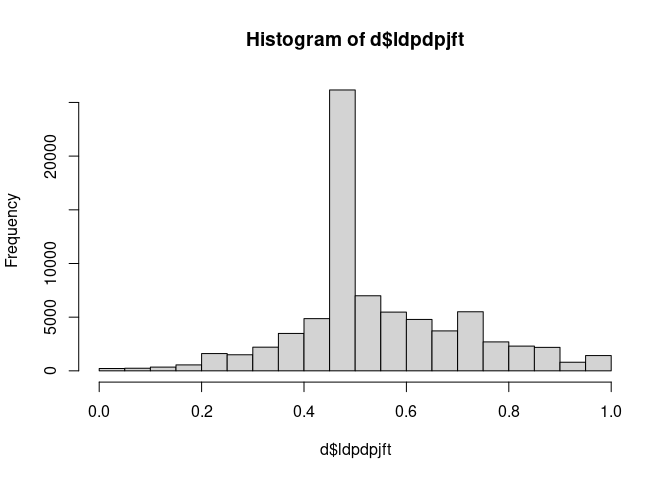
\includegraphics{analysis_4_mediation_matchednoL_v5_files/figure-latex/unnamed-chunk-24-1.pdf}

\begin{Shaded}
\begin{Highlighting}[]
\KeywordTok{ggsave}\NormalTok{(}\KeywordTok{paste0}\NormalTok{(projdir,}\StringTok{"/out/mediationplot_familiarityFT_KOR_matchednoL_v5.png"}\NormalTok{),p,}\DataTypeTok{width=}\DecValTok{8}\NormalTok{,}\DataTypeTok{height=}\DecValTok{5}\NormalTok{)}
\end{Highlighting}
\end{Shaded}

\begin{verbatim}
## Warning: position_dodge requires non-overlapping x intervals

## Warning: position_dodge requires non-overlapping x intervals

## Warning: position_dodge requires non-overlapping x intervals

## Warning: position_dodge requires non-overlapping x intervals

## Warning: position_dodge requires non-overlapping x intervals

## Warning: position_dodge requires non-overlapping x intervals

## Warning: position_dodge requires non-overlapping x intervals

## Warning: position_dodge requires non-overlapping x intervals
\end{verbatim}

\begin{Shaded}
\begin{Highlighting}[]
\KeywordTok{require}\NormalTok{(ggplot2)}
\NormalTok{p <-}\StringTok{ }\KeywordTok{ggplot}\NormalTok{(coefdt[coefdt}\OperatorTok{$}\NormalTok{med}\OperatorTok{==}\StringTok{"familiarityFT_KOR"} \OperatorTok{&}\StringTok{ }\NormalTok{coefdt}\OperatorTok{$}\NormalTok{mod}\OperatorTok{!=}\StringTok{"Treatment => Outcome}\CharTok{\textbackslash{}n}\StringTok{(ADE)"}\NormalTok{,], }\KeywordTok{aes}\NormalTok{(}\DataTypeTok{x=}\NormalTok{gender, }\DataTypeTok{y=}\NormalTok{est)) }\OperatorTok{+}
\StringTok{  }\KeywordTok{geom_hline}\NormalTok{(}\KeywordTok{aes}\NormalTok{(}\DataTypeTok{yintercept=}\DecValTok{0}\NormalTok{), }\DataTypeTok{linetype=}\DecValTok{2}\NormalTok{) }\OperatorTok{+}
\StringTok{  }\KeywordTok{geom_errorbar}\NormalTok{(}\KeywordTok{aes}\NormalTok{(}\DataTypeTok{ymin=}\NormalTok{lci95,}\DataTypeTok{ymax=}\NormalTok{uci95,}\DataTypeTok{colour=}\KeywordTok{as.factor}\NormalTok{(age), }\DataTypeTok{alpha=}\NormalTok{pstar), }
                \DataTypeTok{position=}\KeywordTok{position_dodge}\NormalTok{(}\DataTypeTok{width=}\OperatorTok{-}\FloatTok{0.7}\NormalTok{), }\DataTypeTok{size=}\FloatTok{0.5}\NormalTok{, }\DataTypeTok{width=}\FloatTok{0.3}\NormalTok{) }\OperatorTok{+}
\StringTok{  }\KeywordTok{geom_errorbar}\NormalTok{(}\KeywordTok{aes}\NormalTok{(}\DataTypeTok{ymin=}\NormalTok{lci90,}\DataTypeTok{ymax=}\NormalTok{uci90,}\DataTypeTok{colour=}\KeywordTok{as.factor}\NormalTok{(age), }\DataTypeTok{alpha=}\NormalTok{pstar),}
                \DataTypeTok{position=}\KeywordTok{position_dodge}\NormalTok{(}\DataTypeTok{width=}\OperatorTok{-}\FloatTok{0.7}\NormalTok{), }\DataTypeTok{size=}\FloatTok{1.5}\NormalTok{, }\DataTypeTok{width=}\FloatTok{0.0}\NormalTok{) }\OperatorTok{+}
\StringTok{  }\KeywordTok{geom_point}\NormalTok{(}\KeywordTok{aes}\NormalTok{(}\DataTypeTok{shape=}\KeywordTok{as.factor}\NormalTok{(age), }\DataTypeTok{colour=}\KeywordTok{as.factor}\NormalTok{(age), }\DataTypeTok{alpha=}\NormalTok{pstar),}
             \DataTypeTok{position=}\KeywordTok{position_dodge}\NormalTok{(}\DataTypeTok{width=}\OperatorTok{-}\FloatTok{0.7}\NormalTok{), }\DataTypeTok{size=}\DecValTok{3}\NormalTok{) }\OperatorTok{+}
\StringTok{  }\KeywordTok{facet_grid}\NormalTok{(gender }\OperatorTok{~}\StringTok{ }\NormalTok{mod, }\DataTypeTok{scales =} \StringTok{"free"}\NormalTok{) }\OperatorTok{+}
\StringTok{  }\KeywordTok{scale_alpha_manual}\NormalTok{(}\DataTypeTok{name=}\StringTok{"Significance"}\NormalTok{,}\DataTypeTok{values=}\KeywordTok{c}\NormalTok{(}\DecValTok{1}\NormalTok{,}\FloatTok{0.5}\NormalTok{,}\FloatTok{0.2}\NormalTok{), }\DataTypeTok{drop=}\OtherTok{FALSE}\NormalTok{) }\OperatorTok{+}
\StringTok{  }\KeywordTok{scale_shape_discrete}\NormalTok{(}\DataTypeTok{name=}\StringTok{"Age"}\NormalTok{) }\OperatorTok{+}
\StringTok{  }\KeywordTok{scale_color_manual}\NormalTok{(}\DataTypeTok{name=}\StringTok{"Age"}\NormalTok{,}\DataTypeTok{values=}\KeywordTok{rep}\NormalTok{(}\StringTok{"black"}\NormalTok{, }\DecValTok{5}\NormalTok{)) }\OperatorTok{+}
\StringTok{  }\KeywordTok{ylab}\NormalTok{(}\StringTok{"(Thin Line = 95% CI; Thick Line 90% CI)"}\NormalTok{) }\OperatorTok{+}
\StringTok{  }\KeywordTok{xlab}\NormalTok{(}\OtherTok{NULL}\NormalTok{) }\OperatorTok{+}
\StringTok{  }\KeywordTok{labs}\NormalTok{(}\DataTypeTok{caption=}\StringTok{"Treatment: University education (1:attained, 0:not attained). }\CharTok{\textbackslash{}n}\StringTok{Mediatior: South Korea Feeling Thermometer (rescaled to 0-1 with 1 being the most favorable).}\CharTok{\textbackslash{}n}\StringTok{Outcome: Agreement with granting suffrage to permanent residents (rescaled to 0-1)."}\NormalTok{) }\OperatorTok{+}
\StringTok{  }\KeywordTok{coord_flip}\NormalTok{() }\OperatorTok{+}\StringTok{ }\KeywordTok{theme_bw}\NormalTok{() }\OperatorTok{+}
\StringTok{  }\KeywordTok{theme}\NormalTok{(}\DataTypeTok{legend.position =} \StringTok{"bottom"}\NormalTok{,}
        \DataTypeTok{strip.text.x =} \KeywordTok{element_text}\NormalTok{(}\DataTypeTok{size=}\DecValTok{9}\NormalTok{),}
        \DataTypeTok{strip.text.y =} \KeywordTok{element_text}\NormalTok{(}\DataTypeTok{angle=}\DecValTok{0}\NormalTok{,}\DataTypeTok{size=}\DecValTok{11}\NormalTok{),}
        \DataTypeTok{strip.background =} \KeywordTok{element_rect}\NormalTok{(}\DataTypeTok{fill=}\OtherTok{NA}\NormalTok{,}\DataTypeTok{color=}\OtherTok{NA}\NormalTok{),}
        \DataTypeTok{plot.caption =} \KeywordTok{element_text}\NormalTok{(}\DataTypeTok{hjust=}\DecValTok{0}\NormalTok{),}
        \DataTypeTok{plot.subtitle =} \KeywordTok{element_text}\NormalTok{(}\DataTypeTok{hjust=}\FloatTok{0.5}\NormalTok{),}
        \DataTypeTok{axis.text.y =} \KeywordTok{element_blank}\NormalTok{(),}
        \DataTypeTok{axis.ticks.y =} \KeywordTok{element_blank}\NormalTok{())}
\NormalTok{p}
\end{Highlighting}
\end{Shaded}

\begin{verbatim}
## Warning: position_dodge requires non-overlapping x intervals

## Warning: position_dodge requires non-overlapping x intervals

## Warning: position_dodge requires non-overlapping x intervals

## Warning: position_dodge requires non-overlapping x intervals

## Warning: position_dodge requires non-overlapping x intervals

## Warning: position_dodge requires non-overlapping x intervals
\end{verbatim}

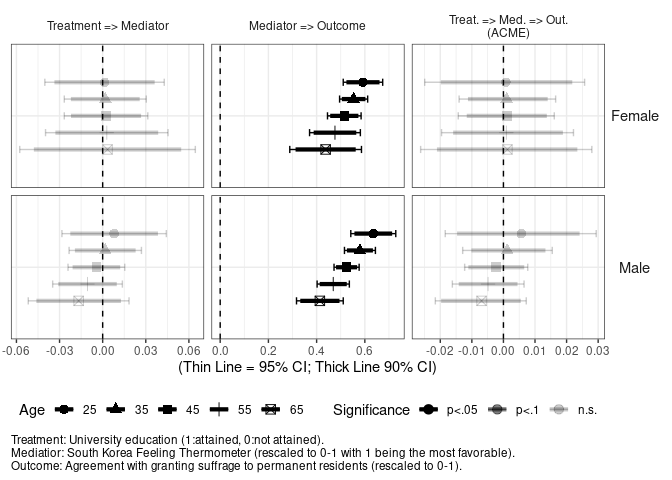
\includegraphics{analysis_4_mediation_matchednoL_v5_files/figure-latex/unnamed-chunk-24-2.pdf}

\begin{Shaded}
\begin{Highlighting}[]
\KeywordTok{ggsave}\NormalTok{(}\KeywordTok{paste0}\NormalTok{(projdir,}\StringTok{"/out/mediationplot2_familiarityFT_KOR_matchednoL_v5.png"}\NormalTok{),p,}\DataTypeTok{width=}\DecValTok{8}\NormalTok{,}\DataTypeTok{height=}\DecValTok{5}\NormalTok{)}
\end{Highlighting}
\end{Shaded}

\begin{verbatim}
## Warning: position_dodge requires non-overlapping x intervals

## Warning: position_dodge requires non-overlapping x intervals

## Warning: position_dodge requires non-overlapping x intervals

## Warning: position_dodge requires non-overlapping x intervals

## Warning: position_dodge requires non-overlapping x intervals

## Warning: position_dodge requires non-overlapping x intervals
\end{verbatim}

\hypertarget{plotting-for-china-feeling-thermometer}{%
\subsection{Plotting for China Feeling
Thermometer}\label{plotting-for-china-feeling-thermometer}}

\begin{Shaded}
\begin{Highlighting}[]
\KeywordTok{require}\NormalTok{(ggplot2)}
\NormalTok{p <-}\StringTok{ }\KeywordTok{ggplot}\NormalTok{(coefdt[coefdt}\OperatorTok{$}\NormalTok{med}\OperatorTok{==}\StringTok{"familiarityFT_CHN"}\NormalTok{,], }\KeywordTok{aes}\NormalTok{(}\DataTypeTok{x=}\NormalTok{gender, }\DataTypeTok{y=}\NormalTok{est)) }\OperatorTok{+}
\StringTok{  }\KeywordTok{geom_hline}\NormalTok{(}\KeywordTok{aes}\NormalTok{(}\DataTypeTok{yintercept=}\DecValTok{0}\NormalTok{), }\DataTypeTok{linetype=}\DecValTok{2}\NormalTok{) }\OperatorTok{+}
\StringTok{  }\KeywordTok{geom_errorbar}\NormalTok{(}\KeywordTok{aes}\NormalTok{(}\DataTypeTok{ymin=}\NormalTok{lci95,}\DataTypeTok{ymax=}\NormalTok{uci95,}\DataTypeTok{colour=}\KeywordTok{as.factor}\NormalTok{(age), }\DataTypeTok{alpha=}\NormalTok{pstar), }
                \DataTypeTok{position=}\KeywordTok{position_dodge}\NormalTok{(}\DataTypeTok{width=}\OperatorTok{-}\FloatTok{0.7}\NormalTok{), }\DataTypeTok{size=}\FloatTok{0.5}\NormalTok{, }\DataTypeTok{width=}\FloatTok{0.3}\NormalTok{) }\OperatorTok{+}
\StringTok{  }\KeywordTok{geom_errorbar}\NormalTok{(}\KeywordTok{aes}\NormalTok{(}\DataTypeTok{ymin=}\NormalTok{lci90,}\DataTypeTok{ymax=}\NormalTok{uci90,}\DataTypeTok{colour=}\KeywordTok{as.factor}\NormalTok{(age), }\DataTypeTok{alpha=}\NormalTok{pstar),}
                \DataTypeTok{position=}\KeywordTok{position_dodge}\NormalTok{(}\DataTypeTok{width=}\OperatorTok{-}\FloatTok{0.7}\NormalTok{), }\DataTypeTok{size=}\FloatTok{1.5}\NormalTok{, }\DataTypeTok{width=}\FloatTok{0.0}\NormalTok{) }\OperatorTok{+}
\StringTok{  }\KeywordTok{geom_point}\NormalTok{(}\KeywordTok{aes}\NormalTok{(}\DataTypeTok{shape=}\KeywordTok{as.factor}\NormalTok{(age), }\DataTypeTok{colour=}\KeywordTok{as.factor}\NormalTok{(age), }\DataTypeTok{alpha=}\NormalTok{pstar),}
             \DataTypeTok{position=}\KeywordTok{position_dodge}\NormalTok{(}\DataTypeTok{width=}\OperatorTok{-}\FloatTok{0.7}\NormalTok{), }\DataTypeTok{size=}\DecValTok{3}\NormalTok{) }\OperatorTok{+}
\StringTok{  }\KeywordTok{facet_grid}\NormalTok{(gender }\OperatorTok{~}\StringTok{ }\NormalTok{mod, }\DataTypeTok{scales =} \StringTok{"free"}\NormalTok{) }\OperatorTok{+}
\StringTok{  }\KeywordTok{scale_alpha_manual}\NormalTok{(}\DataTypeTok{name=}\StringTok{"Significance"}\NormalTok{,}\DataTypeTok{values=}\KeywordTok{c}\NormalTok{(}\DecValTok{1}\NormalTok{,}\FloatTok{0.5}\NormalTok{,}\FloatTok{0.2}\NormalTok{), }\DataTypeTok{drop=}\OtherTok{FALSE}\NormalTok{) }\OperatorTok{+}
\StringTok{  }\KeywordTok{scale_shape_discrete}\NormalTok{(}\DataTypeTok{name=}\StringTok{"Age"}\NormalTok{) }\OperatorTok{+}
\StringTok{  }\KeywordTok{scale_color_manual}\NormalTok{(}\DataTypeTok{name=}\StringTok{"Age"}\NormalTok{,}\DataTypeTok{values=}\KeywordTok{rep}\NormalTok{(}\StringTok{"black"}\NormalTok{, }\DecValTok{5}\NormalTok{)) }\OperatorTok{+}
\StringTok{  }\KeywordTok{ylab}\NormalTok{(}\StringTok{"(Thin Line = 95% CI; Thick Line 90% CI)"}\NormalTok{) }\OperatorTok{+}
\StringTok{  }\KeywordTok{xlab}\NormalTok{(}\OtherTok{NULL}\NormalTok{) }\OperatorTok{+}
\StringTok{  }\KeywordTok{labs}\NormalTok{(}\DataTypeTok{caption=}\StringTok{"Treatment: University education (1:attained, 0:not attained). }\CharTok{\textbackslash{}n}\StringTok{Mediatior: China Feeling Thermometer (rescaled to 0-1 with 1 being the most favorable).}\CharTok{\textbackslash{}n}\StringTok{Outcome: Agreement with granting suffrage to permanent residents (rescaled to 0-1)."}\NormalTok{) }\OperatorTok{+}
\StringTok{  }\KeywordTok{coord_flip}\NormalTok{() }\OperatorTok{+}\StringTok{ }\KeywordTok{theme_bw}\NormalTok{() }\OperatorTok{+}
\StringTok{  }\KeywordTok{theme}\NormalTok{(}\DataTypeTok{legend.position =} \StringTok{"bottom"}\NormalTok{,}
        \DataTypeTok{strip.text.x =} \KeywordTok{element_text}\NormalTok{(}\DataTypeTok{size=}\DecValTok{9}\NormalTok{),}
        \DataTypeTok{strip.text.y =} \KeywordTok{element_text}\NormalTok{(}\DataTypeTok{angle=}\DecValTok{0}\NormalTok{,}\DataTypeTok{size=}\DecValTok{11}\NormalTok{),}
        \DataTypeTok{strip.background =} \KeywordTok{element_rect}\NormalTok{(}\DataTypeTok{fill=}\OtherTok{NA}\NormalTok{,}\DataTypeTok{color=}\OtherTok{NA}\NormalTok{),}
        \DataTypeTok{plot.caption =} \KeywordTok{element_text}\NormalTok{(}\DataTypeTok{hjust=}\DecValTok{0}\NormalTok{),}
        \DataTypeTok{plot.subtitle =} \KeywordTok{element_text}\NormalTok{(}\DataTypeTok{hjust=}\FloatTok{0.5}\NormalTok{),}
        \DataTypeTok{axis.text.y =} \KeywordTok{element_blank}\NormalTok{(),}
        \DataTypeTok{axis.ticks.y =} \KeywordTok{element_blank}\NormalTok{())}
\NormalTok{p}
\end{Highlighting}
\end{Shaded}

\begin{verbatim}
## Warning: position_dodge requires non-overlapping x intervals

## Warning: position_dodge requires non-overlapping x intervals

## Warning: position_dodge requires non-overlapping x intervals

## Warning: position_dodge requires non-overlapping x intervals

## Warning: position_dodge requires non-overlapping x intervals

## Warning: position_dodge requires non-overlapping x intervals

## Warning: position_dodge requires non-overlapping x intervals

## Warning: position_dodge requires non-overlapping x intervals
\end{verbatim}

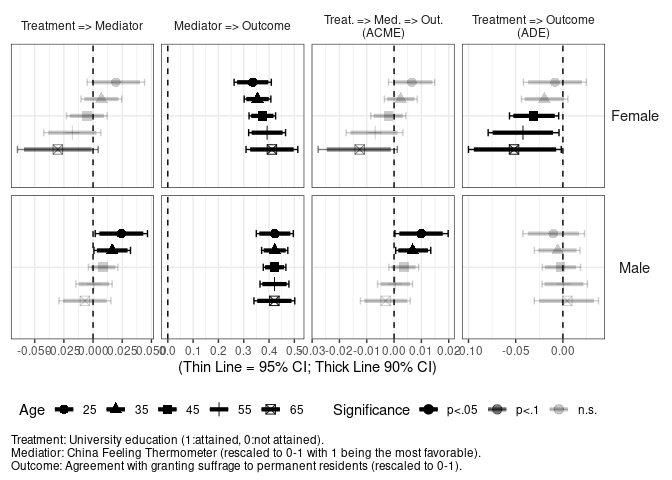
\includegraphics{analysis_4_mediation_matchednoL_v5_files/figure-latex/unnamed-chunk-25-1.pdf}

\begin{Shaded}
\begin{Highlighting}[]
\KeywordTok{ggsave}\NormalTok{(}\KeywordTok{paste0}\NormalTok{(projdir,}\StringTok{"/out/mediationplot_familiarityFT_CHN_matchednoL_v5.png"}\NormalTok{),p,}\DataTypeTok{width=}\DecValTok{8}\NormalTok{,}\DataTypeTok{height=}\DecValTok{5}\NormalTok{)}
\end{Highlighting}
\end{Shaded}

\begin{verbatim}
## Warning: position_dodge requires non-overlapping x intervals

## Warning: position_dodge requires non-overlapping x intervals

## Warning: position_dodge requires non-overlapping x intervals

## Warning: position_dodge requires non-overlapping x intervals

## Warning: position_dodge requires non-overlapping x intervals

## Warning: position_dodge requires non-overlapping x intervals

## Warning: position_dodge requires non-overlapping x intervals

## Warning: position_dodge requires non-overlapping x intervals
\end{verbatim}

\begin{Shaded}
\begin{Highlighting}[]
\KeywordTok{require}\NormalTok{(ggplot2)}
\NormalTok{p <-}\StringTok{ }\KeywordTok{ggplot}\NormalTok{(coefdt[coefdt}\OperatorTok{$}\NormalTok{med}\OperatorTok{==}\StringTok{"familiarityFT_CHN"} \OperatorTok{&}\StringTok{ }\NormalTok{coefdt}\OperatorTok{$}\NormalTok{mod}\OperatorTok{!=}\StringTok{"Treatment => Outcome}\CharTok{\textbackslash{}n}\StringTok{(ADE)"}\NormalTok{,], }\KeywordTok{aes}\NormalTok{(}\DataTypeTok{x=}\NormalTok{gender, }\DataTypeTok{y=}\NormalTok{est)) }\OperatorTok{+}
\StringTok{  }\KeywordTok{geom_hline}\NormalTok{(}\KeywordTok{aes}\NormalTok{(}\DataTypeTok{yintercept=}\DecValTok{0}\NormalTok{), }\DataTypeTok{linetype=}\DecValTok{2}\NormalTok{) }\OperatorTok{+}
\StringTok{  }\KeywordTok{geom_errorbar}\NormalTok{(}\KeywordTok{aes}\NormalTok{(}\DataTypeTok{ymin=}\NormalTok{lci95,}\DataTypeTok{ymax=}\NormalTok{uci95,}\DataTypeTok{colour=}\KeywordTok{as.factor}\NormalTok{(age), }\DataTypeTok{alpha=}\NormalTok{pstar), }
                \DataTypeTok{position=}\KeywordTok{position_dodge}\NormalTok{(}\DataTypeTok{width=}\OperatorTok{-}\FloatTok{0.7}\NormalTok{), }\DataTypeTok{size=}\FloatTok{0.5}\NormalTok{, }\DataTypeTok{width=}\FloatTok{0.3}\NormalTok{) }\OperatorTok{+}
\StringTok{  }\KeywordTok{geom_errorbar}\NormalTok{(}\KeywordTok{aes}\NormalTok{(}\DataTypeTok{ymin=}\NormalTok{lci90,}\DataTypeTok{ymax=}\NormalTok{uci90,}\DataTypeTok{colour=}\KeywordTok{as.factor}\NormalTok{(age), }\DataTypeTok{alpha=}\NormalTok{pstar),}
                \DataTypeTok{position=}\KeywordTok{position_dodge}\NormalTok{(}\DataTypeTok{width=}\OperatorTok{-}\FloatTok{0.7}\NormalTok{), }\DataTypeTok{size=}\FloatTok{1.5}\NormalTok{, }\DataTypeTok{width=}\FloatTok{0.0}\NormalTok{) }\OperatorTok{+}
\StringTok{  }\KeywordTok{geom_point}\NormalTok{(}\KeywordTok{aes}\NormalTok{(}\DataTypeTok{shape=}\KeywordTok{as.factor}\NormalTok{(age), }\DataTypeTok{colour=}\KeywordTok{as.factor}\NormalTok{(age), }\DataTypeTok{alpha=}\NormalTok{pstar),}
             \DataTypeTok{position=}\KeywordTok{position_dodge}\NormalTok{(}\DataTypeTok{width=}\OperatorTok{-}\FloatTok{0.7}\NormalTok{), }\DataTypeTok{size=}\DecValTok{3}\NormalTok{) }\OperatorTok{+}
\StringTok{  }\KeywordTok{facet_grid}\NormalTok{(gender }\OperatorTok{~}\StringTok{ }\NormalTok{mod, }\DataTypeTok{scales =} \StringTok{"free"}\NormalTok{) }\OperatorTok{+}
\StringTok{  }\KeywordTok{scale_alpha_manual}\NormalTok{(}\DataTypeTok{name=}\StringTok{"Significance"}\NormalTok{,}\DataTypeTok{values=}\KeywordTok{c}\NormalTok{(}\DecValTok{1}\NormalTok{,}\FloatTok{0.5}\NormalTok{,}\FloatTok{0.2}\NormalTok{), }\DataTypeTok{drop=}\OtherTok{FALSE}\NormalTok{) }\OperatorTok{+}
\StringTok{  }\KeywordTok{scale_shape_discrete}\NormalTok{(}\DataTypeTok{name=}\StringTok{"Age"}\NormalTok{) }\OperatorTok{+}
\StringTok{  }\KeywordTok{scale_color_manual}\NormalTok{(}\DataTypeTok{name=}\StringTok{"Age"}\NormalTok{,}\DataTypeTok{values=}\KeywordTok{rep}\NormalTok{(}\StringTok{"black"}\NormalTok{, }\DecValTok{5}\NormalTok{)) }\OperatorTok{+}
\StringTok{  }\KeywordTok{ylab}\NormalTok{(}\StringTok{"(Thin Line = 95% CI; Thick Line 90% CI)"}\NormalTok{) }\OperatorTok{+}
\StringTok{  }\KeywordTok{xlab}\NormalTok{(}\OtherTok{NULL}\NormalTok{) }\OperatorTok{+}
\StringTok{  }\KeywordTok{labs}\NormalTok{(}\DataTypeTok{caption=}\StringTok{"Treatment: University education (1:attained, 0:not attained). }\CharTok{\textbackslash{}n}\StringTok{Mediatior: China Feeling Thermometer (rescaled to 0-1 with 1 being the most favorable).}\CharTok{\textbackslash{}n}\StringTok{Outcome: Agreement with granting suffrage to permanent residents (rescaled to 0-1)."}\NormalTok{) }\OperatorTok{+}
\StringTok{  }\KeywordTok{coord_flip}\NormalTok{() }\OperatorTok{+}\StringTok{ }\KeywordTok{theme_bw}\NormalTok{() }\OperatorTok{+}
\StringTok{  }\KeywordTok{theme}\NormalTok{(}\DataTypeTok{legend.position =} \StringTok{"bottom"}\NormalTok{,}
        \DataTypeTok{strip.text.x =} \KeywordTok{element_text}\NormalTok{(}\DataTypeTok{size=}\DecValTok{9}\NormalTok{),}
        \DataTypeTok{strip.text.y =} \KeywordTok{element_text}\NormalTok{(}\DataTypeTok{angle=}\DecValTok{0}\NormalTok{,}\DataTypeTok{size=}\DecValTok{11}\NormalTok{),}
        \DataTypeTok{strip.background =} \KeywordTok{element_rect}\NormalTok{(}\DataTypeTok{fill=}\OtherTok{NA}\NormalTok{,}\DataTypeTok{color=}\OtherTok{NA}\NormalTok{),}
        \DataTypeTok{plot.caption =} \KeywordTok{element_text}\NormalTok{(}\DataTypeTok{hjust=}\DecValTok{0}\NormalTok{),}
        \DataTypeTok{plot.subtitle =} \KeywordTok{element_text}\NormalTok{(}\DataTypeTok{hjust=}\FloatTok{0.5}\NormalTok{),}
        \DataTypeTok{axis.text.y =} \KeywordTok{element_blank}\NormalTok{(),}
        \DataTypeTok{axis.ticks.y =} \KeywordTok{element_blank}\NormalTok{())}
\NormalTok{p}
\end{Highlighting}
\end{Shaded}

\begin{verbatim}
## Warning: position_dodge requires non-overlapping x intervals

## Warning: position_dodge requires non-overlapping x intervals

## Warning: position_dodge requires non-overlapping x intervals

## Warning: position_dodge requires non-overlapping x intervals

## Warning: position_dodge requires non-overlapping x intervals

## Warning: position_dodge requires non-overlapping x intervals
\end{verbatim}

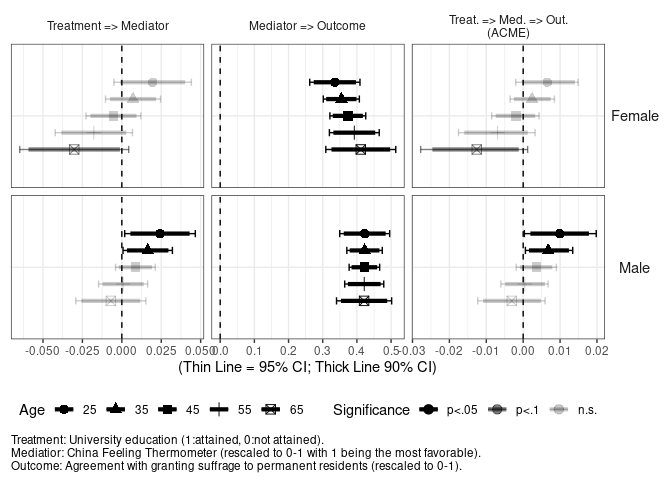
\includegraphics{analysis_4_mediation_matchednoL_v5_files/figure-latex/unnamed-chunk-25-2.pdf}

\begin{Shaded}
\begin{Highlighting}[]
\KeywordTok{ggsave}\NormalTok{(}\KeywordTok{paste0}\NormalTok{(projdir,}\StringTok{"/out/mediationplot2_familiarityFT_CHN_matchednoL_v5.png"}\NormalTok{),p,}\DataTypeTok{width=}\DecValTok{8}\NormalTok{,}\DataTypeTok{height=}\DecValTok{5}\NormalTok{)}
\end{Highlighting}
\end{Shaded}

\begin{verbatim}
## Warning: position_dodge requires non-overlapping x intervals

## Warning: position_dodge requires non-overlapping x intervals

## Warning: position_dodge requires non-overlapping x intervals

## Warning: position_dodge requires non-overlapping x intervals

## Warning: position_dodge requires non-overlapping x intervals

## Warning: position_dodge requires non-overlapping x intervals
\end{verbatim}

\hypertarget{plotting-for-united-states-feeling-thermometer}{%
\subsection{Plotting for United States Feeling
Thermometer}\label{plotting-for-united-states-feeling-thermometer}}

\begin{Shaded}
\begin{Highlighting}[]
\KeywordTok{require}\NormalTok{(ggplot2)}
\NormalTok{p <-}\StringTok{ }\KeywordTok{ggplot}\NormalTok{(coefdt[coefdt}\OperatorTok{$}\NormalTok{med}\OperatorTok{==}\StringTok{"familiarityFT_USA"}\NormalTok{,], }\KeywordTok{aes}\NormalTok{(}\DataTypeTok{x=}\NormalTok{gender, }\DataTypeTok{y=}\NormalTok{est)) }\OperatorTok{+}
\StringTok{  }\KeywordTok{geom_hline}\NormalTok{(}\KeywordTok{aes}\NormalTok{(}\DataTypeTok{yintercept=}\DecValTok{0}\NormalTok{), }\DataTypeTok{linetype=}\DecValTok{2}\NormalTok{) }\OperatorTok{+}
\StringTok{  }\KeywordTok{geom_errorbar}\NormalTok{(}\KeywordTok{aes}\NormalTok{(}\DataTypeTok{ymin=}\NormalTok{lci95,}\DataTypeTok{ymax=}\NormalTok{uci95,}\DataTypeTok{colour=}\KeywordTok{as.factor}\NormalTok{(age), }\DataTypeTok{alpha=}\NormalTok{pstar), }
                \DataTypeTok{position=}\KeywordTok{position_dodge}\NormalTok{(}\DataTypeTok{width=}\OperatorTok{-}\FloatTok{0.7}\NormalTok{), }\DataTypeTok{size=}\FloatTok{0.5}\NormalTok{, }\DataTypeTok{width=}\FloatTok{0.3}\NormalTok{) }\OperatorTok{+}
\StringTok{  }\KeywordTok{geom_errorbar}\NormalTok{(}\KeywordTok{aes}\NormalTok{(}\DataTypeTok{ymin=}\NormalTok{lci90,}\DataTypeTok{ymax=}\NormalTok{uci90,}\DataTypeTok{colour=}\KeywordTok{as.factor}\NormalTok{(age), }\DataTypeTok{alpha=}\NormalTok{pstar),}
                \DataTypeTok{position=}\KeywordTok{position_dodge}\NormalTok{(}\DataTypeTok{width=}\OperatorTok{-}\FloatTok{0.7}\NormalTok{), }\DataTypeTok{size=}\FloatTok{1.5}\NormalTok{, }\DataTypeTok{width=}\FloatTok{0.0}\NormalTok{) }\OperatorTok{+}
\StringTok{  }\KeywordTok{geom_point}\NormalTok{(}\KeywordTok{aes}\NormalTok{(}\DataTypeTok{shape=}\KeywordTok{as.factor}\NormalTok{(age), }\DataTypeTok{colour=}\KeywordTok{as.factor}\NormalTok{(age), }\DataTypeTok{alpha=}\NormalTok{pstar),}
             \DataTypeTok{position=}\KeywordTok{position_dodge}\NormalTok{(}\DataTypeTok{width=}\OperatorTok{-}\FloatTok{0.7}\NormalTok{), }\DataTypeTok{size=}\DecValTok{3}\NormalTok{) }\OperatorTok{+}
\StringTok{  }\KeywordTok{facet_grid}\NormalTok{(gender }\OperatorTok{~}\StringTok{ }\NormalTok{mod, }\DataTypeTok{scales =} \StringTok{"free"}\NormalTok{) }\OperatorTok{+}
\StringTok{  }\KeywordTok{scale_alpha_manual}\NormalTok{(}\DataTypeTok{name=}\StringTok{"Significance"}\NormalTok{,}\DataTypeTok{values=}\KeywordTok{c}\NormalTok{(}\DecValTok{1}\NormalTok{,}\FloatTok{0.5}\NormalTok{,}\FloatTok{0.2}\NormalTok{), }\DataTypeTok{drop=}\OtherTok{FALSE}\NormalTok{) }\OperatorTok{+}
\StringTok{  }\KeywordTok{scale_shape_discrete}\NormalTok{(}\DataTypeTok{name=}\StringTok{"Age"}\NormalTok{) }\OperatorTok{+}
\StringTok{  }\KeywordTok{scale_color_manual}\NormalTok{(}\DataTypeTok{name=}\StringTok{"Age"}\NormalTok{,}\DataTypeTok{values=}\KeywordTok{rep}\NormalTok{(}\StringTok{"black"}\NormalTok{, }\DecValTok{5}\NormalTok{)) }\OperatorTok{+}
\StringTok{  }\KeywordTok{ylab}\NormalTok{(}\StringTok{"(Thin Line = 95% CI; Thick Line 90% CI)"}\NormalTok{) }\OperatorTok{+}
\StringTok{  }\KeywordTok{xlab}\NormalTok{(}\OtherTok{NULL}\NormalTok{) }\OperatorTok{+}
\StringTok{  }\KeywordTok{labs}\NormalTok{(}\DataTypeTok{caption=}\StringTok{"Treatment: University education (1:attained, 0:not attained). }\CharTok{\textbackslash{}n}\StringTok{Mediatior: United States Feeling Thermometer (rescaled to 0-1 with 1 being the most favorable).}\CharTok{\textbackslash{}n}\StringTok{Outcome: Agreement with granting suffrage to permanent residents (rescaled to 0-1)."}\NormalTok{) }\OperatorTok{+}
\StringTok{  }\KeywordTok{coord_flip}\NormalTok{() }\OperatorTok{+}\StringTok{ }\KeywordTok{theme_bw}\NormalTok{() }\OperatorTok{+}
\StringTok{  }\KeywordTok{theme}\NormalTok{(}\DataTypeTok{legend.position =} \StringTok{"bottom"}\NormalTok{,}
        \DataTypeTok{strip.text.x =} \KeywordTok{element_text}\NormalTok{(}\DataTypeTok{size=}\DecValTok{9}\NormalTok{),}
        \DataTypeTok{strip.text.y =} \KeywordTok{element_text}\NormalTok{(}\DataTypeTok{angle=}\DecValTok{0}\NormalTok{,}\DataTypeTok{size=}\DecValTok{11}\NormalTok{),}
        \DataTypeTok{strip.background =} \KeywordTok{element_rect}\NormalTok{(}\DataTypeTok{fill=}\OtherTok{NA}\NormalTok{,}\DataTypeTok{color=}\OtherTok{NA}\NormalTok{),}
        \DataTypeTok{plot.caption =} \KeywordTok{element_text}\NormalTok{(}\DataTypeTok{hjust=}\DecValTok{0}\NormalTok{),}
        \DataTypeTok{plot.subtitle =} \KeywordTok{element_text}\NormalTok{(}\DataTypeTok{hjust=}\FloatTok{0.5}\NormalTok{),}
        \DataTypeTok{axis.text.y =} \KeywordTok{element_blank}\NormalTok{(),}
        \DataTypeTok{axis.ticks.y =} \KeywordTok{element_blank}\NormalTok{())}
\NormalTok{p}
\end{Highlighting}
\end{Shaded}

\begin{verbatim}
## Warning: position_dodge requires non-overlapping x intervals

## Warning: position_dodge requires non-overlapping x intervals

## Warning: position_dodge requires non-overlapping x intervals

## Warning: position_dodge requires non-overlapping x intervals

## Warning: position_dodge requires non-overlapping x intervals

## Warning: position_dodge requires non-overlapping x intervals

## Warning: position_dodge requires non-overlapping x intervals

## Warning: position_dodge requires non-overlapping x intervals
\end{verbatim}

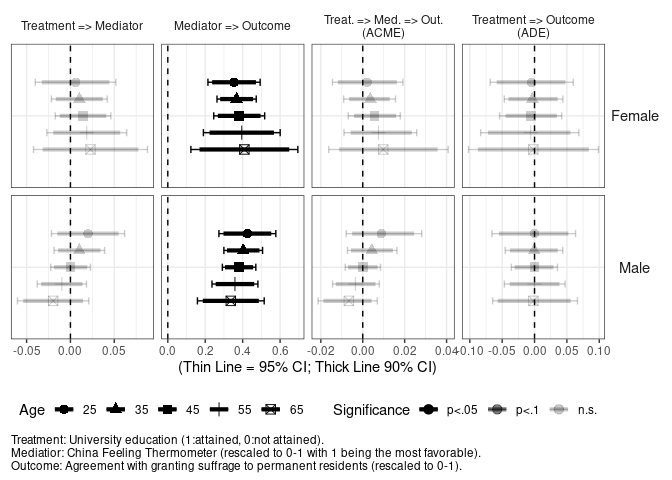
\includegraphics{analysis_4_mediation_matchednoL_v5_files/figure-latex/unnamed-chunk-26-1.pdf}

\begin{Shaded}
\begin{Highlighting}[]
\KeywordTok{ggsave}\NormalTok{(}\KeywordTok{paste0}\NormalTok{(projdir,}\StringTok{"/out/mediationplot_familiarityFT_USA_matchednoL_v5.png"}\NormalTok{),p,}\DataTypeTok{width=}\DecValTok{8}\NormalTok{,}\DataTypeTok{height=}\DecValTok{5}\NormalTok{)}
\end{Highlighting}
\end{Shaded}

\begin{verbatim}
## Warning: position_dodge requires non-overlapping x intervals

## Warning: position_dodge requires non-overlapping x intervals

## Warning: position_dodge requires non-overlapping x intervals

## Warning: position_dodge requires non-overlapping x intervals

## Warning: position_dodge requires non-overlapping x intervals

## Warning: position_dodge requires non-overlapping x intervals

## Warning: position_dodge requires non-overlapping x intervals

## Warning: position_dodge requires non-overlapping x intervals
\end{verbatim}

\begin{Shaded}
\begin{Highlighting}[]
\KeywordTok{require}\NormalTok{(ggplot2)}
\NormalTok{p <-}\StringTok{ }\KeywordTok{ggplot}\NormalTok{(coefdt[coefdt}\OperatorTok{$}\NormalTok{med}\OperatorTok{==}\StringTok{"familiarityFT_USA"} \OperatorTok{&}\StringTok{ }\NormalTok{coefdt}\OperatorTok{$}\NormalTok{mod}\OperatorTok{!=}\StringTok{"Treatment => Outcome}\CharTok{\textbackslash{}n}\StringTok{(ADE)"}\NormalTok{,], }\KeywordTok{aes}\NormalTok{(}\DataTypeTok{x=}\NormalTok{gender, }\DataTypeTok{y=}\NormalTok{est)) }\OperatorTok{+}
\StringTok{  }\KeywordTok{geom_hline}\NormalTok{(}\KeywordTok{aes}\NormalTok{(}\DataTypeTok{yintercept=}\DecValTok{0}\NormalTok{), }\DataTypeTok{linetype=}\DecValTok{2}\NormalTok{) }\OperatorTok{+}
\StringTok{  }\KeywordTok{geom_errorbar}\NormalTok{(}\KeywordTok{aes}\NormalTok{(}\DataTypeTok{ymin=}\NormalTok{lci95,}\DataTypeTok{ymax=}\NormalTok{uci95,}\DataTypeTok{colour=}\KeywordTok{as.factor}\NormalTok{(age), }\DataTypeTok{alpha=}\NormalTok{pstar), }
                \DataTypeTok{position=}\KeywordTok{position_dodge}\NormalTok{(}\DataTypeTok{width=}\OperatorTok{-}\FloatTok{0.7}\NormalTok{), }\DataTypeTok{size=}\FloatTok{0.5}\NormalTok{, }\DataTypeTok{width=}\FloatTok{0.3}\NormalTok{) }\OperatorTok{+}
\StringTok{  }\KeywordTok{geom_errorbar}\NormalTok{(}\KeywordTok{aes}\NormalTok{(}\DataTypeTok{ymin=}\NormalTok{lci90,}\DataTypeTok{ymax=}\NormalTok{uci90,}\DataTypeTok{colour=}\KeywordTok{as.factor}\NormalTok{(age), }\DataTypeTok{alpha=}\NormalTok{pstar),}
                \DataTypeTok{position=}\KeywordTok{position_dodge}\NormalTok{(}\DataTypeTok{width=}\OperatorTok{-}\FloatTok{0.7}\NormalTok{), }\DataTypeTok{size=}\FloatTok{1.5}\NormalTok{, }\DataTypeTok{width=}\FloatTok{0.0}\NormalTok{) }\OperatorTok{+}
\StringTok{  }\KeywordTok{geom_point}\NormalTok{(}\KeywordTok{aes}\NormalTok{(}\DataTypeTok{shape=}\KeywordTok{as.factor}\NormalTok{(age), }\DataTypeTok{colour=}\KeywordTok{as.factor}\NormalTok{(age), }\DataTypeTok{alpha=}\NormalTok{pstar),}
             \DataTypeTok{position=}\KeywordTok{position_dodge}\NormalTok{(}\DataTypeTok{width=}\OperatorTok{-}\FloatTok{0.7}\NormalTok{), }\DataTypeTok{size=}\DecValTok{3}\NormalTok{) }\OperatorTok{+}
\StringTok{  }\KeywordTok{facet_grid}\NormalTok{(gender }\OperatorTok{~}\StringTok{ }\NormalTok{mod, }\DataTypeTok{scales =} \StringTok{"free"}\NormalTok{) }\OperatorTok{+}
\StringTok{  }\KeywordTok{scale_alpha_manual}\NormalTok{(}\DataTypeTok{name=}\StringTok{"Significance"}\NormalTok{,}\DataTypeTok{values=}\KeywordTok{c}\NormalTok{(}\DecValTok{1}\NormalTok{,}\FloatTok{0.5}\NormalTok{,}\FloatTok{0.2}\NormalTok{), }\DataTypeTok{drop=}\OtherTok{FALSE}\NormalTok{) }\OperatorTok{+}
\StringTok{  }\KeywordTok{scale_shape_discrete}\NormalTok{(}\DataTypeTok{name=}\StringTok{"Age"}\NormalTok{) }\OperatorTok{+}
\StringTok{  }\KeywordTok{scale_color_manual}\NormalTok{(}\DataTypeTok{name=}\StringTok{"Age"}\NormalTok{,}\DataTypeTok{values=}\KeywordTok{rep}\NormalTok{(}\StringTok{"black"}\NormalTok{, }\DecValTok{5}\NormalTok{)) }\OperatorTok{+}
\StringTok{  }\KeywordTok{ylab}\NormalTok{(}\StringTok{"(Thin Line = 95% CI; Thick Line 90% CI)"}\NormalTok{) }\OperatorTok{+}
\StringTok{  }\KeywordTok{xlab}\NormalTok{(}\OtherTok{NULL}\NormalTok{) }\OperatorTok{+}
\StringTok{  }\KeywordTok{labs}\NormalTok{(}\DataTypeTok{caption=}\StringTok{"Treatment: University education (1:attained, 0:not attained). }\CharTok{\textbackslash{}n}\StringTok{Mediatior: United States Feeling Thermometer (rescaled to 0-1 with 1 being the most favorable).}\CharTok{\textbackslash{}n}\StringTok{Outcome: Agreement with granting suffrage to permanent residents (rescaled to 0-1)."}\NormalTok{) }\OperatorTok{+}
\StringTok{  }\KeywordTok{coord_flip}\NormalTok{() }\OperatorTok{+}\StringTok{ }\KeywordTok{theme_bw}\NormalTok{() }\OperatorTok{+}
\StringTok{  }\KeywordTok{theme}\NormalTok{(}\DataTypeTok{legend.position =} \StringTok{"bottom"}\NormalTok{,}
        \DataTypeTok{strip.text.x =} \KeywordTok{element_text}\NormalTok{(}\DataTypeTok{size=}\DecValTok{9}\NormalTok{),}
        \DataTypeTok{strip.text.y =} \KeywordTok{element_text}\NormalTok{(}\DataTypeTok{angle=}\DecValTok{0}\NormalTok{,}\DataTypeTok{size=}\DecValTok{11}\NormalTok{),}
        \DataTypeTok{strip.background =} \KeywordTok{element_rect}\NormalTok{(}\DataTypeTok{fill=}\OtherTok{NA}\NormalTok{,}\DataTypeTok{color=}\OtherTok{NA}\NormalTok{),}
        \DataTypeTok{plot.caption =} \KeywordTok{element_text}\NormalTok{(}\DataTypeTok{hjust=}\DecValTok{0}\NormalTok{),}
        \DataTypeTok{plot.subtitle =} \KeywordTok{element_text}\NormalTok{(}\DataTypeTok{hjust=}\FloatTok{0.5}\NormalTok{),}
        \DataTypeTok{axis.text.y =} \KeywordTok{element_blank}\NormalTok{(),}
        \DataTypeTok{axis.ticks.y =} \KeywordTok{element_blank}\NormalTok{())}
\NormalTok{p}
\end{Highlighting}
\end{Shaded}

\begin{verbatim}
## Warning: position_dodge requires non-overlapping x intervals

## Warning: position_dodge requires non-overlapping x intervals

## Warning: position_dodge requires non-overlapping x intervals

## Warning: position_dodge requires non-overlapping x intervals

## Warning: position_dodge requires non-overlapping x intervals

## Warning: position_dodge requires non-overlapping x intervals
\end{verbatim}

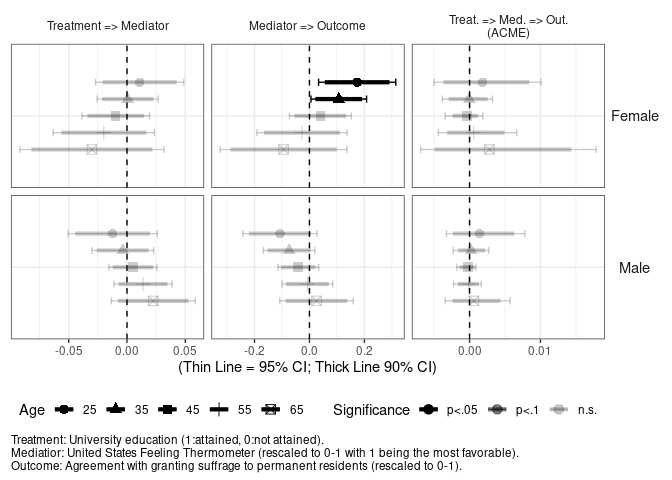
\includegraphics{analysis_4_mediation_matchednoL_v5_files/figure-latex/unnamed-chunk-26-2.pdf}

\begin{Shaded}
\begin{Highlighting}[]
\KeywordTok{ggsave}\NormalTok{(}\KeywordTok{paste0}\NormalTok{(projdir,}\StringTok{"/out/mediationplot2_familiarityFT_USA_matchednoL_v5.png"}\NormalTok{),p,}\DataTypeTok{width=}\DecValTok{8}\NormalTok{,}\DataTypeTok{height=}\DecValTok{5}\NormalTok{)}
\end{Highlighting}
\end{Shaded}

\begin{verbatim}
## Warning: position_dodge requires non-overlapping x intervals

## Warning: position_dodge requires non-overlapping x intervals

## Warning: position_dodge requires non-overlapping x intervals

## Warning: position_dodge requires non-overlapping x intervals

## Warning: position_dodge requires non-overlapping x intervals

## Warning: position_dodge requires non-overlapping x intervals
\end{verbatim}

\hypertarget{plotting-for-income}{%
\subsection{Plotting for Income}\label{plotting-for-income}}

\begin{Shaded}
\begin{Highlighting}[]
\KeywordTok{require}\NormalTok{(ggplot2)}
\NormalTok{p <-}\StringTok{ }\KeywordTok{ggplot}\NormalTok{(coefdt[coefdt}\OperatorTok{$}\NormalTok{med}\OperatorTok{==}\StringTok{"income"}\NormalTok{,], }\KeywordTok{aes}\NormalTok{(}\DataTypeTok{x=}\NormalTok{gender, }\DataTypeTok{y=}\NormalTok{est)) }\OperatorTok{+}
\StringTok{  }\KeywordTok{geom_hline}\NormalTok{(}\KeywordTok{aes}\NormalTok{(}\DataTypeTok{yintercept=}\DecValTok{0}\NormalTok{), }\DataTypeTok{linetype=}\DecValTok{2}\NormalTok{) }\OperatorTok{+}
\StringTok{  }\KeywordTok{geom_errorbar}\NormalTok{(}\KeywordTok{aes}\NormalTok{(}\DataTypeTok{ymin=}\NormalTok{lci95,}\DataTypeTok{ymax=}\NormalTok{uci95,}\DataTypeTok{colour=}\KeywordTok{as.factor}\NormalTok{(age), }\DataTypeTok{alpha=}\NormalTok{pstar), }
                \DataTypeTok{position=}\KeywordTok{position_dodge}\NormalTok{(}\DataTypeTok{width=}\OperatorTok{-}\FloatTok{0.7}\NormalTok{), }\DataTypeTok{size=}\FloatTok{0.5}\NormalTok{, }\DataTypeTok{width=}\FloatTok{0.3}\NormalTok{) }\OperatorTok{+}
\StringTok{  }\KeywordTok{geom_errorbar}\NormalTok{(}\KeywordTok{aes}\NormalTok{(}\DataTypeTok{ymin=}\NormalTok{lci90,}\DataTypeTok{ymax=}\NormalTok{uci90,}\DataTypeTok{colour=}\KeywordTok{as.factor}\NormalTok{(age), }\DataTypeTok{alpha=}\NormalTok{pstar),}
                \DataTypeTok{position=}\KeywordTok{position_dodge}\NormalTok{(}\DataTypeTok{width=}\OperatorTok{-}\FloatTok{0.7}\NormalTok{), }\DataTypeTok{size=}\FloatTok{1.5}\NormalTok{, }\DataTypeTok{width=}\FloatTok{0.0}\NormalTok{) }\OperatorTok{+}
\StringTok{  }\KeywordTok{geom_point}\NormalTok{(}\KeywordTok{aes}\NormalTok{(}\DataTypeTok{shape=}\KeywordTok{as.factor}\NormalTok{(age), }\DataTypeTok{colour=}\KeywordTok{as.factor}\NormalTok{(age), }\DataTypeTok{alpha=}\NormalTok{pstar),}
             \DataTypeTok{position=}\KeywordTok{position_dodge}\NormalTok{(}\DataTypeTok{width=}\OperatorTok{-}\FloatTok{0.7}\NormalTok{), }\DataTypeTok{size=}\DecValTok{3}\NormalTok{) }\OperatorTok{+}
\StringTok{  }\KeywordTok{facet_grid}\NormalTok{(gender }\OperatorTok{~}\StringTok{ }\NormalTok{mod, }\DataTypeTok{scales =} \StringTok{"free"}\NormalTok{) }\OperatorTok{+}
\StringTok{  }\KeywordTok{scale_alpha_manual}\NormalTok{(}\DataTypeTok{name=}\StringTok{"Significance"}\NormalTok{,}\DataTypeTok{values=}\KeywordTok{c}\NormalTok{(}\DecValTok{1}\NormalTok{,}\FloatTok{0.5}\NormalTok{,}\FloatTok{0.2}\NormalTok{), }\DataTypeTok{drop=}\OtherTok{FALSE}\NormalTok{) }\OperatorTok{+}
\StringTok{  }\KeywordTok{scale_shape_discrete}\NormalTok{(}\DataTypeTok{name=}\StringTok{"Age"}\NormalTok{) }\OperatorTok{+}
\StringTok{  }\KeywordTok{scale_color_manual}\NormalTok{(}\DataTypeTok{name=}\StringTok{"Age"}\NormalTok{,}\DataTypeTok{values=}\KeywordTok{rep}\NormalTok{(}\StringTok{"black"}\NormalTok{, }\DecValTok{5}\NormalTok{)) }\OperatorTok{+}
\StringTok{  }\KeywordTok{ylab}\NormalTok{(}\StringTok{"(Thin Line = 95% CI; Thick Line 90% CI)"}\NormalTok{) }\OperatorTok{+}
\StringTok{  }\KeywordTok{xlab}\NormalTok{(}\OtherTok{NULL}\NormalTok{) }\OperatorTok{+}
\StringTok{  }\KeywordTok{labs}\NormalTok{(}\DataTypeTok{caption=}\StringTok{"Treatment: University education (1:attained, 0:not attained). }\CharTok{\textbackslash{}n}\StringTok{Mediatior: Income (rescaled to 0-1 with 1 being the richest).}\CharTok{\textbackslash{}n}\StringTok{Outcome: Agreement with granting suffrage to permanent residents (rescaled to 0-1)."}\NormalTok{) }\OperatorTok{+}
\StringTok{  }\KeywordTok{coord_flip}\NormalTok{() }\OperatorTok{+}\StringTok{ }\KeywordTok{theme_bw}\NormalTok{() }\OperatorTok{+}
\StringTok{  }\KeywordTok{theme}\NormalTok{(}\DataTypeTok{legend.position =} \StringTok{"bottom"}\NormalTok{,}
        \DataTypeTok{strip.text.x =} \KeywordTok{element_text}\NormalTok{(}\DataTypeTok{size=}\DecValTok{9}\NormalTok{),}
        \DataTypeTok{strip.text.y =} \KeywordTok{element_text}\NormalTok{(}\DataTypeTok{angle=}\DecValTok{0}\NormalTok{,}\DataTypeTok{size=}\DecValTok{11}\NormalTok{),}
        \DataTypeTok{strip.background =} \KeywordTok{element_rect}\NormalTok{(}\DataTypeTok{fill=}\OtherTok{NA}\NormalTok{,}\DataTypeTok{color=}\OtherTok{NA}\NormalTok{),}
        \DataTypeTok{plot.caption =} \KeywordTok{element_text}\NormalTok{(}\DataTypeTok{hjust=}\DecValTok{0}\NormalTok{),}
        \DataTypeTok{plot.subtitle =} \KeywordTok{element_text}\NormalTok{(}\DataTypeTok{hjust=}\FloatTok{0.5}\NormalTok{),}
        \DataTypeTok{axis.text.y =} \KeywordTok{element_blank}\NormalTok{(),}
        \DataTypeTok{axis.ticks.y =} \KeywordTok{element_blank}\NormalTok{())}
\NormalTok{p}
\end{Highlighting}
\end{Shaded}

\begin{verbatim}
## Warning: position_dodge requires non-overlapping x intervals

## Warning: position_dodge requires non-overlapping x intervals

## Warning: position_dodge requires non-overlapping x intervals

## Warning: position_dodge requires non-overlapping x intervals

## Warning: position_dodge requires non-overlapping x intervals

## Warning: position_dodge requires non-overlapping x intervals

## Warning: position_dodge requires non-overlapping x intervals

## Warning: position_dodge requires non-overlapping x intervals
\end{verbatim}

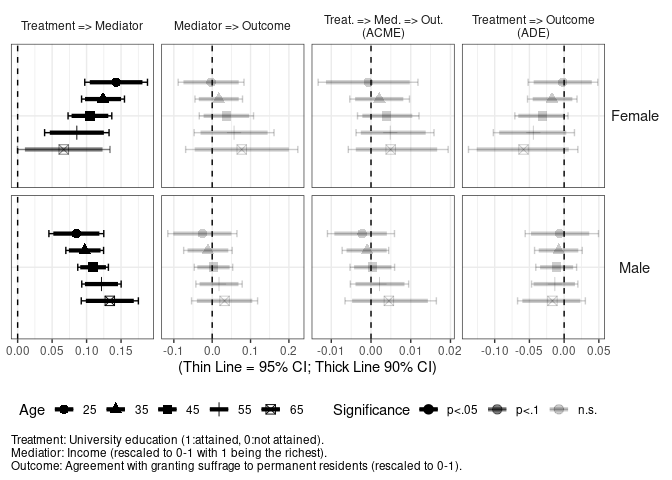
\includegraphics{analysis_4_mediation_matchednoL_v5_files/figure-latex/unnamed-chunk-27-1.pdf}

\begin{Shaded}
\begin{Highlighting}[]
\KeywordTok{ggsave}\NormalTok{(}\KeywordTok{paste0}\NormalTok{(projdir,}\StringTok{"/out/mediationplot_income_matchednoL_v5.png"}\NormalTok{),p,}\DataTypeTok{width=}\DecValTok{8}\NormalTok{,}\DataTypeTok{height=}\DecValTok{5}\NormalTok{)}
\end{Highlighting}
\end{Shaded}

\begin{verbatim}
## Warning: position_dodge requires non-overlapping x intervals

## Warning: position_dodge requires non-overlapping x intervals

## Warning: position_dodge requires non-overlapping x intervals

## Warning: position_dodge requires non-overlapping x intervals

## Warning: position_dodge requires non-overlapping x intervals

## Warning: position_dodge requires non-overlapping x intervals

## Warning: position_dodge requires non-overlapping x intervals

## Warning: position_dodge requires non-overlapping x intervals
\end{verbatim}

\begin{Shaded}
\begin{Highlighting}[]
\KeywordTok{require}\NormalTok{(ggplot2)}
\NormalTok{p <-}\StringTok{ }\KeywordTok{ggplot}\NormalTok{(coefdt[coefdt}\OperatorTok{$}\NormalTok{med}\OperatorTok{==}\StringTok{"income"} \OperatorTok{&}\StringTok{ }\NormalTok{coefdt}\OperatorTok{$}\NormalTok{mod}\OperatorTok{!=}\StringTok{"Treatment => Outcome}\CharTok{\textbackslash{}n}\StringTok{(ADE)"}\NormalTok{,], }\KeywordTok{aes}\NormalTok{(}\DataTypeTok{x=}\NormalTok{gender, }\DataTypeTok{y=}\NormalTok{est)) }\OperatorTok{+}
\StringTok{  }\KeywordTok{geom_hline}\NormalTok{(}\KeywordTok{aes}\NormalTok{(}\DataTypeTok{yintercept=}\DecValTok{0}\NormalTok{), }\DataTypeTok{linetype=}\DecValTok{2}\NormalTok{) }\OperatorTok{+}
\StringTok{  }\KeywordTok{geom_errorbar}\NormalTok{(}\KeywordTok{aes}\NormalTok{(}\DataTypeTok{ymin=}\NormalTok{lci95,}\DataTypeTok{ymax=}\NormalTok{uci95,}\DataTypeTok{colour=}\KeywordTok{as.factor}\NormalTok{(age), }\DataTypeTok{alpha=}\NormalTok{pstar), }
                \DataTypeTok{position=}\KeywordTok{position_dodge}\NormalTok{(}\DataTypeTok{width=}\OperatorTok{-}\FloatTok{0.7}\NormalTok{), }\DataTypeTok{size=}\FloatTok{0.5}\NormalTok{, }\DataTypeTok{width=}\FloatTok{0.3}\NormalTok{) }\OperatorTok{+}
\StringTok{  }\KeywordTok{geom_errorbar}\NormalTok{(}\KeywordTok{aes}\NormalTok{(}\DataTypeTok{ymin=}\NormalTok{lci90,}\DataTypeTok{ymax=}\NormalTok{uci90,}\DataTypeTok{colour=}\KeywordTok{as.factor}\NormalTok{(age), }\DataTypeTok{alpha=}\NormalTok{pstar),}
                \DataTypeTok{position=}\KeywordTok{position_dodge}\NormalTok{(}\DataTypeTok{width=}\OperatorTok{-}\FloatTok{0.7}\NormalTok{), }\DataTypeTok{size=}\FloatTok{1.5}\NormalTok{, }\DataTypeTok{width=}\FloatTok{0.0}\NormalTok{) }\OperatorTok{+}
\StringTok{  }\KeywordTok{geom_point}\NormalTok{(}\KeywordTok{aes}\NormalTok{(}\DataTypeTok{shape=}\KeywordTok{as.factor}\NormalTok{(age), }\DataTypeTok{colour=}\KeywordTok{as.factor}\NormalTok{(age), }\DataTypeTok{alpha=}\NormalTok{pstar),}
             \DataTypeTok{position=}\KeywordTok{position_dodge}\NormalTok{(}\DataTypeTok{width=}\OperatorTok{-}\FloatTok{0.7}\NormalTok{), }\DataTypeTok{size=}\DecValTok{3}\NormalTok{) }\OperatorTok{+}
\StringTok{  }\KeywordTok{facet_grid}\NormalTok{(gender }\OperatorTok{~}\StringTok{ }\NormalTok{mod, }\DataTypeTok{scales =} \StringTok{"free"}\NormalTok{) }\OperatorTok{+}
\StringTok{  }\KeywordTok{scale_alpha_manual}\NormalTok{(}\DataTypeTok{name=}\StringTok{"Significance"}\NormalTok{,}\DataTypeTok{values=}\KeywordTok{c}\NormalTok{(}\DecValTok{1}\NormalTok{,}\FloatTok{0.5}\NormalTok{,}\FloatTok{0.2}\NormalTok{), }\DataTypeTok{drop=}\OtherTok{FALSE}\NormalTok{) }\OperatorTok{+}
\StringTok{  }\KeywordTok{scale_shape_discrete}\NormalTok{(}\DataTypeTok{name=}\StringTok{"Age"}\NormalTok{) }\OperatorTok{+}
\StringTok{  }\KeywordTok{scale_color_manual}\NormalTok{(}\DataTypeTok{name=}\StringTok{"Age"}\NormalTok{,}\DataTypeTok{values=}\KeywordTok{rep}\NormalTok{(}\StringTok{"black"}\NormalTok{, }\DecValTok{5}\NormalTok{)) }\OperatorTok{+}
\StringTok{  }\KeywordTok{ylab}\NormalTok{(}\StringTok{"(Thin Line = 95% CI; Thick Line 90% CI)"}\NormalTok{) }\OperatorTok{+}
\StringTok{  }\KeywordTok{xlab}\NormalTok{(}\OtherTok{NULL}\NormalTok{) }\OperatorTok{+}
\StringTok{  }\KeywordTok{labs}\NormalTok{(}\DataTypeTok{caption=}\StringTok{"Treatment: University education (1:attained, 0:not attained). }\CharTok{\textbackslash{}n}\StringTok{Mediatior: Income (rescaled to 0-1 with 1 being the richest).}\CharTok{\textbackslash{}n}\StringTok{Outcome: Agreement with granting suffrage to permanent residents (rescaled to 0-1)."}\NormalTok{) }\OperatorTok{+}
\StringTok{  }\KeywordTok{coord_flip}\NormalTok{() }\OperatorTok{+}\StringTok{ }\KeywordTok{theme_bw}\NormalTok{() }\OperatorTok{+}
\StringTok{  }\KeywordTok{theme}\NormalTok{(}\DataTypeTok{legend.position =} \StringTok{"bottom"}\NormalTok{,}
        \DataTypeTok{strip.text.x =} \KeywordTok{element_text}\NormalTok{(}\DataTypeTok{size=}\DecValTok{9}\NormalTok{),}
        \DataTypeTok{strip.text.y =} \KeywordTok{element_text}\NormalTok{(}\DataTypeTok{angle=}\DecValTok{0}\NormalTok{,}\DataTypeTok{size=}\DecValTok{11}\NormalTok{),}
        \DataTypeTok{strip.background =} \KeywordTok{element_rect}\NormalTok{(}\DataTypeTok{fill=}\OtherTok{NA}\NormalTok{,}\DataTypeTok{color=}\OtherTok{NA}\NormalTok{),}
        \DataTypeTok{plot.caption =} \KeywordTok{element_text}\NormalTok{(}\DataTypeTok{hjust=}\DecValTok{0}\NormalTok{),}
        \DataTypeTok{plot.subtitle =} \KeywordTok{element_text}\NormalTok{(}\DataTypeTok{hjust=}\FloatTok{0.5}\NormalTok{),}
        \DataTypeTok{axis.text.y =} \KeywordTok{element_blank}\NormalTok{(),}
        \DataTypeTok{axis.ticks.y =} \KeywordTok{element_blank}\NormalTok{())}
\NormalTok{p}
\end{Highlighting}
\end{Shaded}

\begin{verbatim}
## Warning: position_dodge requires non-overlapping x intervals

## Warning: position_dodge requires non-overlapping x intervals

## Warning: position_dodge requires non-overlapping x intervals

## Warning: position_dodge requires non-overlapping x intervals

## Warning: position_dodge requires non-overlapping x intervals

## Warning: position_dodge requires non-overlapping x intervals
\end{verbatim}

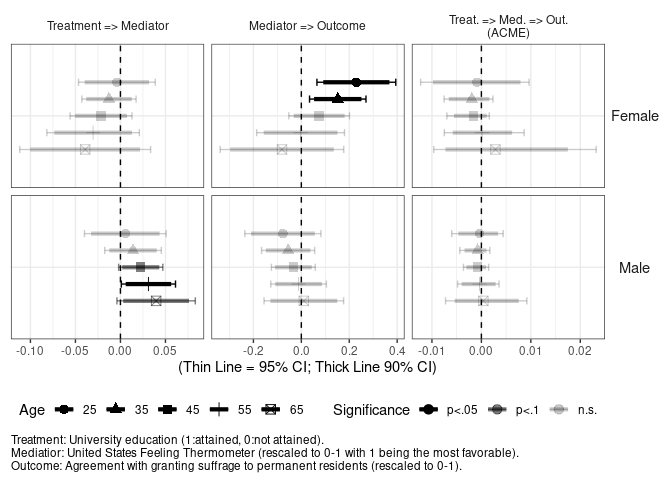
\includegraphics{analysis_4_mediation_matchednoL_v5_files/figure-latex/unnamed-chunk-27-2.pdf}

\begin{Shaded}
\begin{Highlighting}[]
\KeywordTok{ggsave}\NormalTok{(}\KeywordTok{paste0}\NormalTok{(projdir,}\StringTok{"/out/mediationplot2_income_matchednoL_v5.png"}\NormalTok{),p,}\DataTypeTok{width=}\DecValTok{8}\NormalTok{,}\DataTypeTok{height=}\DecValTok{5}\NormalTok{)}
\end{Highlighting}
\end{Shaded}

\begin{verbatim}
## Warning: position_dodge requires non-overlapping x intervals

## Warning: position_dodge requires non-overlapping x intervals

## Warning: position_dodge requires non-overlapping x intervals

## Warning: position_dodge requires non-overlapping x intervals

## Warning: position_dodge requires non-overlapping x intervals

## Warning: position_dodge requires non-overlapping x intervals
\end{verbatim}

\end{document}
